\documentclass[FM,DP]{tulthesis}

% fonts, langs, packages...
\usepackage{polyglossia}
\setdefaultlanguage{czech}
\usepackage{fontspec}
\usepackage{xunicode}
\usepackage{xltxtra}
\setsansfont[Mapping=tex-text,BoldFont={* Bold},Numbers=OldStyle]{Myriad Pro}
\usepackage{hyperref}
\hypersetup{colorlinks=true, linkcolor=tul, urlcolor=tul, citecolor=tul}
\usepackage{graphicx}
\usepackage{mathtools}
\usepackage{booktabs}
\usepackage{listings}
\usepackage[toc,page]{appendix}
\usepackage{amsmath}
\usepackage{amssymb}
\newcommand{\argument}[1]{{\ttfamily\color{\tulcolor}#1}}
\newcommand{\prikaz}[1]{\argument{\textbackslash #1}}
\newenvironment{myquote}{\begin{list}{}{\setlength\leftmargin\parindent}\item[]}{\end{list}}
\sloppy

\usepackage{array}
\newcolumntype{L}[1]{>{\raggedright\let\newline\\\arraybackslash\hspace{0pt}}m{#1}}
\newcolumntype{C}[1]{>{\centering\let\newline\\\arraybackslash\hspace{0pt}}m{#1}}
\newcolumntype{R}[1]{>{\raggedleft\let\newline\\\arraybackslash\hspace{0pt}}m{#1}}

% syntax highlighting
\usepackage[newfloat]{minted}
\usepackage[labelfont=bf,font=it]{caption}
\usepackage{etoolbox}
\definecolor{bg}{rgb}{0.95,0.95,0.95}
\setminted{bgcolor=bg, frame=single, rulecolor=\color{bg}, breaklines=true}
\makeatletter
\patchcmd{\minted@colorbg}{\noindent}{\medskip\noindent}{}{}
\apptocmd{\endminted@colorbg}{\par\medskip}{}{}
\makeatother
\newenvironment{code}
    {\filbreak\captionsetup{type=listing}}{\filbreak}
\SetupFloatingEnvironment{listing}{name=Výpis}
\renewcommand{\floatpagefraction}{.8}%

% brak lines in \url{}
\makeatletter
\g@addto@macro{\UrlBreaks}{\UrlOrds}
\makeatother


%%%%%%%%%%%%%%%%%%%%%%%%%%%%
\TULtitle{Vyhledávání jako služba}{Search as a Service}
\TULprogramme{Aplikovaná informatika}{Applied Informatics}
\TULbranch{Informační systémy a technologie}{Information Technologies}
\TULauthor{Bc. Luděk Veselý}
\TULsupervisor{Prof. Ing. Zdeněk Molnár, CSc.}
\TULreader{Ing. Ivan Jelínek}
\TULyear{2017}

\renewcommand{\listlistingname}{Seznam výpisů programů}


%%%%%%%%%%%%%%%%%%%%%%%%%%%%
\begin{document}
\pagenumbering{gobble}
\ThesisStart{male}


%%%%%%%%%%%%%%%%%%%%%%%%%%%%
\begin{acknowledgement}
Rád bych poděkoval Prof. Ing. Zdeňkovi Molnárovi, CSc. za vedení mé diplomové práce
a veškerou pomoc při jejím řešení.
\end{acknowledgement}


%%%%%%%%%%%%%%%%%%%%%%%%%%%%
\begin{abstractCZ}
Tato diplomová práce se zabývá návrhem a tvorbou plnotextového vyhledávání, které je poskytováno jako služba, 
přičemž samotné vyhledávání se zaměřuje na~použití v~elektronických obchodech. V~úvodu práce je analyzována 
problematika elektronického obchodování, jsou vysvětleny související pojmy a definovány požadavky na~samotné 
vyhledávání. Následně jsou popsány teoretické možnosti textového vyhledávání pro~dané použití. Na~základě
analýzy je vytvořen návrh aplikace, který je následně implementován v~programovacím jazyce Go s~využitím 
nástroje Elasticsearch. V závěru práce je aplikace testována, čímž je ověřeno splnění požadavků na~vyhledávání
z~pohledu kvality vyhledávání, rychlosti i uživatelské přívětivosti služby.
\end{abstractCZ}
\vspace{1cm}
\begin{klicovaslovaCZ}
Plnotextové vyhledávání, software jako služba, elektronický obchod, Elasticsearch
\end{klicovaslovaCZ}

\vspace{2cm}

\begin{abstractEN}
This thesis is focused on design and implementation of fulltext searching, which is provided as a servise. 
The searching itself is focused on the utilization in e-shops. At the beginning, the question of e-commerce 
is analysed, the related terms are explained and the requirements of searching are identified. Then, the 
theoretical ways of text searching in this context are described. On the analyse is created a conception 
of application, which is further implemented in the language Go with the usage of Elasticresearch. 
Finally, the application is tested, which should examine not only the quality and speed of searching 
but also the user-friendliness.
\end{abstractEN}
\vspace{1cm}
\begin{klicovaslovaEN}
Full text search, Software as a service, E-shop, Elasticsearch
\end{klicovaslovaEN}


%%%%%%%%%%%%%%%%%%%%%%%%%%%%
\pagenumbering{roman}
\setcounter{page}{2}
\addcontentsline{toc}{chapter}{Obsah}
\tableofcontents
\clearpage

% obrazky
\addcontentsline{toc}{chapter}{Seznam obrázků}
\listoffigures
\clearpage

% tabulky
\addcontentsline{toc}{chapter}{Seznam tabulek}
\listoftables
\clearpage

% vypisy programu
\addcontentsline{toc}{chapter}{Seznam výpisů programů}
\listoflistings
\clearpage


%%%%%%%%%%%%%%%%%%%%%%%%%%%%
\pagenumbering{arabic}
\chapter{Úvod}

Vyhledávání  je jednou z klíčových funkcí elektronického obchodu. Umožňuje rychlé nalezení
hledaného produktu, což přináší zákazníkům úsporu času a usnadňuje tak orientaci na webu.
Textové vyhledávání však není snadné implementovat, protože je třeba si poradit se zpracováním
přirozeného jazyka a dalšími problémy -- je totiž vhodné mít určitou úroveň znalosti principů samotného 
vyhledávání včetně souvisejících oborů a technologií. Implementace kvalitního vyhledávání
tak může být pro provozovatele elektronického obchodu náročná jak časově, tak finančně.

Tento nástroj je poskytován jako služba se všemi výhodami i omezeními s tímto principem spojenými. 
Měl by provozovatelům elektronických obchodů usnadnit implementaci vyhledávání, zároveň
by měl poskytovat tak kvalitní výsledky vyhledávání, aby neměl provozovatel obchodu potřebu
přecházet k jiným nástrojům. Konkrétní cíle diplomové práce jsou popsány v následujících odstavcích.

\section{Cíle práce}

Cílem této práce je \textbf{navrhnout a vytvořit nástroj, který je nabízen jako služba a umožňuje 
provozovatelům elektronických obchodů snadnou implementaci plnotextového vyhledávání do elektronického 
obchodu.} K~dosažení tohoto cíle je třeba naplnit cíle dílčí.

Prvním takovým cílem je provedení analýzy problému a to jak z~pohledu obchodního, tak
z~pohledu samotné problematiky vyhledávání. Co se týče prvního pohledu, je třeba
analyzovat potřeby zákazníků, zjistit, jaká jsou specifika oblasti elektronického obchodování
a definovat kritéria, jejichž naplnění je pro provozovatele elektronických obchodů klíčové. 
Z~pohledu problematiky vyhledávání je třeba provést analýzu této disciplíny a utřídit
tak znalosti potřebné k poskytnutí kvalitních výsledků plnotextového vyhledávání.

Dalším dílčím cílem je vytvořit návrh řešení problému jednak na základě znalosti potřeb
zákazníků a také na základě znalosti problematiky plnotextového vyhledávání. Tento návrh musí 
být v~dalším kroku implementovatelný.

Předposledním dílčím cílem je samotná implementace aplikace dle jejího návrhu. Obnáší to výběr 
vhodných nástrojů, jejich nasazení do produkčního prostředí, naprogramování jednotlivých
služeb a konečně také ověření samotné implementace. Tu je třeba porovnat se stanovenými požadavky
a ověřit tak jejich naplnění. Tento krok potvrdí nebo vyvrátí spránvost implementace.

\section{Cílová skupina}

Cílovou skupinou je chápán ten, komu je určen samotný text této práce, nejde tedy
o~uživatele vzniklé aplikace. 
První cílovou skupinou je vývojář, řešící problém plnotextového vyhledávání produktů 
při implementaci elektronického obchodu. Takovému čtenáři by měla práce poskytnout dostatečné
teoretické znalosti potřebné pro implementaci vyhledávání. Užitečná také může být konkrétní
implementace, která je v této práci popisována.

Další možnou cílovou skupinou je provozovatel elektronického obchodu, který přemýšlí, 
jakým způsobem zlepšit (případně zavést) plnotextové vyhledávání. V~této práci získá 
přehled o~složitosti samotné implementace, poskytne mu komentovaný soupis možných řešení 
a konečně také poskytne funkční službu, kterou může okamžitě na~webový portál napojit.

Poslední cílovou skupinou budiž kdokoli, kdo se zajímá o problematiku plnotextového 
vyhledávání v českém jazyce. V této práci nalezne soupis problémů souvisejicích s češtinou, 
které je třeba řešit. Dále zde nalezne konkrétní implementaci, kterou se může inspirovat 
při řešení obdobného problému.

\section{Použité metody}

V~této části jsou popsány metody použité k~naplnění jednotlivých cílů. Pro zkoumání problému
oboru je provedena analýzu trhu, nabízí se také možnost dotazování potenciálních uživatelů, 
případně je možné vyjít ze zkušeností autora. Pro porozumění problematice vyhledávání 
je provedena rešerše literatury. Vzhledem k množství dostupné literatury bude třeba provést 
syntézu těchto informací. Při vytváření návrhu řešení bude použito modelování, výstupem 
by tedy měl být model řešení. 

\section{Struktura práce}

V první části práce popisuji problematiku vyhledávání v~prostředí elektronického obchodování. 
Definuji zde jednak kontext, v~kterém se pohybuji a dále také popisuji problémy, 
které v~tomto prostředí existují. Snažím se identifikovat potencionálního uživatele 
a definovat jeho požadavky na~plnotextové vyhledávání. Toto prostředí má svá specifika, 
která také popisuji a vysvětluji, proč jsem se na tuto oblast zaměřil. V~závěru této části porovnávám
existující nástroje umožňující implementaci vyhledávání a zjišťuji tak, proč má smysl
vytvářet další službu, jaká je její přidaná hodnota.

V druhé části se zabývám teorií plnotextového vyhledávání. Popisuji zde celý
proces od analýzy vstupních dat, přes jejich indexaci, až po samotné vyhledávání. 
Tyto poznatky budou následně využity k~naplnění požadavků na vyhledávání, k~zajištění
kvalitních výsledků vyhledávání.

V další části práce navrhuji samotnou aplikaci tak, aby vyhovovala požadavkům a zároveň byla 
následně implementovatelná. Porovnávám zde dostupné nástroje, definuji případy užití aplikace
a vytvářím model výsledné aplikace.

Poté popisuji konkrétní implementaci v~jazyce Go s~pomocí úložiště 
Elasticsearch. Výstupem této části je otestovaný spustitelný program, který umožňuje provádět 
indexaci produktů a jejich následné vyhledávání. Tento program je nasazen do produkčního
prostředí a při každé změně zdrojových kódů je aplikace aktualizována.

V poslední části práce je provedeno ověření funkčnosti aplikace, zejména vůči požadavkům na její funkčnost.
Je testována kvalita vyhledávání vzhledem k zpracování přirozeného jazyka, rychlost aplikace
při zátěži a také uživatelská přívětivost, tedy snadnost napojení služby na elektronický obchod.


%%%%%%%%%%%%%%%%%%%%%%%%%%%%
\chapter{Komentovaná rešerše použitých informačních zdrojů}

V této kapitole popisuji jednak práce, které již na VŠE vznikly, avšak od této práce se odlišují.
Dále komentuji literaturu, ze které je nejvíce čerpáno a je tak stěžejním zdrojem informací pro vznik
této práce.

\section{Existující práce obdobného tématu}

Na VŠE již vzniklo několik prací, zabývající se textovým vyhledáváním. Mezi nejpropracovanější
patří \textbf{Návrh vyhledávacího systému pro moderní potřeby} od Bc. Tomáše Maršálka, která
se zabývá implementací vyhledávání, které si dokáže poradit s nepřesným nebo neúplným zadáním 
hledaného výrazu. Výstupem této práce je program, který je možné pro takové vyhledávání použít. 

Další prací zabývající se textovým vyhledáváním je \textbf{Pragmatický lematizátor českých slov} od
Bc. Matěje Vacka. Přestože práce vychází z podobného teoretického základu, jejím výstupem je
opět pouze nástroj pro použití při implementaci vyhledávání. Tato práce se odlišuje v~tom, 
že spíše než vytvoření jednoúčelového nástroje si dává za cíl vytvořit prakticky použitelný
nástroj, který však dílčí části (například zpracování přirozeného jazyka) využívá jako
prostředek k poskytnutí komplexní služby.

\section{Použitá literatura}

Při tvorbě této práce vycházím z literatury uvedené v závěru práce. Teoretické znalosti však
nejvíce čerpám z knihy \textbf{Počítačové zpracování přirozeného jazyka}~\cite{strossa} 
od Petra Strossy, přičemž nejužitečnější pro tuto práci je hned první kapitola 
zabývající se automatizovaným indexováním textů. Knih zabývající se textovým vyhledáváním existuje
celá řada -- dále čerpám především z knih \textbf{Searching in the 21st Century}~\cite{searching}
a \textbf{Mining Text Data}~\cite{mining}.

Dále je třeba mít povědomí o oblasti elektronického obchodování, což je přehledně shrnuto v~knize
\textbf{E-commerce} Petra Suchánka~\cite{e-commerce}. Z této knihy je pro práci nejpřínosnější 
její první polovina, která pojednává jak o obecných termínech, tak je důkladně vysvětluje.

Při návrhu API je třeba mít povědomí o tom jak jej navrhnout i jak jej v konkrétním programovacím 
jazyce implementovat. Obecně o návrhu API pojednává kniha \textbf{Build APIs You Won't Hate} \cite{api},
která je průvodcem návrhu dobře použitelného api od samého počátku, včetně ukázky na konkrétních příkladech.
Pro seznámení s jazykem Go na komplexní úrovni je dostatek informací v knize~\textbf{Go in Action} 
\cite{go-in-action}, která je další z řady knih nakladatelství Manning Publications pojednávající
o řadě dalších nástrojíů. Vzhledem k specifickému užití jazyka jsem čerpal z dalších dvou knih
o tomto programovacím jazyce -- \textbf{Mastering Concurrency in Go} \cite{go-concurrency} a 
\textbf{Build web applications with Golang} \cite{go-xml}. Co se samotného nasazování aplikace týče, 
velmi přínosná je kniha \textbf{The DevOps 2.0 Toolkit} \cite{devops}, která by se dala chápat jako průvodce 
světem DevOps. Přináší spoustu informací pro pochopení tohoto přístupu, což je doloženo řadou 
příkladů. Specielně pro důkladnější porozumění nástroji Docker je k dispozici kniha 
\textbf{Docker: Up \& Running} \cite{docker}, která s tímto nástrojem čtenáře seznámí víc než důkladně.

Vzhledem k použití nástroje Elasticsearch je třeba mít dostatek informací také o tomto nástroji.
Jedna z nejpodrobnějších knih je \textbf{Elasticsearch: The Definitive Guide}, která
popisuje veškerou funkčnost tohoto nástroje a popis doplňuje o teoretické informace nutné
k pochopení dané problematiky. Elasticsearch se však velmi rychle vyvíjí a tak tato kniha
nereflektuje přesně aktuální stav. Konkrétní funkčnost je tedy třeba vždy ověřovat vůči
aktuální dokumentaci \textbf{Elasticsearch Reference}~\cite{elastic-reference}.


%%%%%%%%%%%%%%%%%%%%%%%%%%%%
\chapter{Analýza byznys požadavků na aplikaci}

První část diplomové práce popisuje problematiku plnotextového vyhledávání 
v~prostředí elektronických obchodů. Nejprve je čtenář uveden do problematiky elektronického
obchodování a obeznámen s základními pojmy a principy. Následně je popsán problém, 
který je řešen, a jsou definovány konkrétní podmínky, za kterých bude výsledný nástroj
přínosný a použitelný. Jsou zde také diskutovány stávající možnosti implementace
plnotextového vyhledávání, porovnány alternativní služby a zdůvodněno vytváření nového nástroje.

\section{Vysvětlení základních pojmů}

Pro usnadnění orientace v této práci jsou nejprve vysvětleny dále používané pojmy. Jedná se 
vesměs o známé termíny, přesto je důležité uvést jejich význam na pravou míru.

\subsection*{Elektronické obchodování}

Termín elektronické obchodování (e-commerce) označuje veškerou činnost spojenou s obchodováním
realizovaným prostřednictvím sítě internet \cite[strana~11]{e-commerce}. Spadá sem distribuce, nákup, 
prodej, marketing, servis produktů. Elektronické obchodování se dále podle dělí dle zaměření na cílové 
skupiny, z nichž nejpodstatnější jsou B2C (zaměřeno na koncové zákazníky) a B2B (zaměřeno na obchodníky) 
\cite[strana~17]{e-commerce}. Elektronické obchodování je podmnožinou 
elektronického podnikání (e-business), které oznažuje veškeré obchodní a výrobní aktivity, 
zatímco elektronické obchodování se týká samotného prodeje zboží a služeb.

\subsection*{Elektronický obchod}

Elektronický či internetový obchod (e-shop) je webová aplikace, jejímž prostřednictvím 
provozovatel obchodu prodává zboží nebo služby zákazníkům \cite[strana~16]{e-commerce}.
Jedná se o podmožinu elektronického obchodování, jde tedy o jeden z možných prodejních 
kanálů v prostředí internetu. Elektronický obchod je specifickou webovou aplikací, v~níž 
se opakují určité vzorce. Konkrétně je to katalog produktů, kategorizace zboží, 
vkládání položek do košíku, platba objednávky, možnost kontaktu s~zákaznickou podporou 
prostřednictvím on-line chatu přímo v aplikaci.

V elektronickém obchodě lze shledávat řadu podobností s obchodem kamenným, který zákazníci 
navštěvují osobně. Některé vlastnosti elektronického obchodu jsou zřejmě inspirovány 
obchody kamennými (procházení zboží podle kategorií, přidávání položek do košíku, 
uplatnění slevových poukázek při platbě). Často však elektronický obchod využívá možností, 
které webové prostředí nabízí (filtrace a řazení položek podle parametrů, vrácení se
k naplněnému košíku, porovnávání zboží napříč obchody).

\begin{figure}[h]
\center
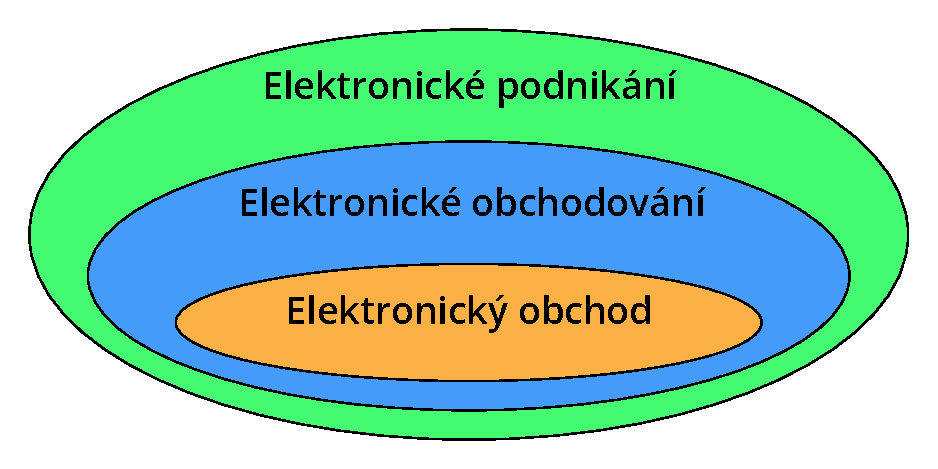
\includegraphics[width=\textwidth]{e-commerce.pdf}
\caption[Vztah elektronického podnikání, obchodování a podnikání]{Vztah elektronického podnikání, obchodování a podnikání (Zdroj: \cite{strossa})}
\label{e-commerce}
\end{figure}

Zcela zásadní výhodou elektronického obchodu oproti návštěvě obchodu kamenného
je možnost vytvoření objednávky z pohodlí domova a její následné doručení zásilkovou 
službou. Tento přístup především šetří čas strávený cestou do obchodu a čas strávený 
v~obchodě. Například v segmentu nákupu potravin může být výhodou to, že je takový 
nákup hygieničtější a zboží bude doručeno v lepším stavu díky uzpůsobeným vozům dopravců.
Výhody ale vznikají i pro provozovatele -- nemusí zřizovat prodejnu včetně jejího vybavení a 
zaměstnance, mohou efektivněji navrhnout sklad, nebo dokonce využít automatizace 
při kompletaci objednaného zboží.

\subsection*{Plnotextové vyhledávání}

Plnotextové vyhledávání (full-text search) je způsob vyhledávání v textových datech, 
kdy se vyhledává uživatelem formulovaný dotaz v invertovaném souboru (někdy také 
indexovém souboru nebo invertovaném indexu), tedy v souboru obsahující výrazy, 
podle nichž je daný záznam jednoduše vyhledatelný \cite[strana~15]{strossa}. 
Proces, kterým vzniká indexový soubor, se nazývá indexace. Tato problematika je podrobněji
popisována v kapitole \ref{ch:indexace}.

\section{Vysvětlení problému, který je řešen}

Plnotextové vyhledávání je rychlým prostředkem nalezení konkrétního produktu
v elektronickém obchodě. Typicky je využito zákazníky, kteří jsou na webu
s konkrétní potřebou a jsou schopni formulovat výraz, podle kterého produkt
hledají. Může jít o název tybu produktu, jeho značku, variantu nebo kategorii.
Pro takového uživatele je procházení webu procházením kategorií zdlouhavé
a právě plnotextové vyhledávání mu může zásadně zrychlit cestu k nalezení 
hledaného produktu.

Důležitost plnotextového vyhledávání navíc roste s rostoucím počtem produktů a kategorií, 
v kterých je složité se orientovat. Uživatel tak může vyhledávání využít už pro 
nalezení kategorie, která se nachází v dlouhém a nepřehledném menu.

\begin{figure}[h]
\center
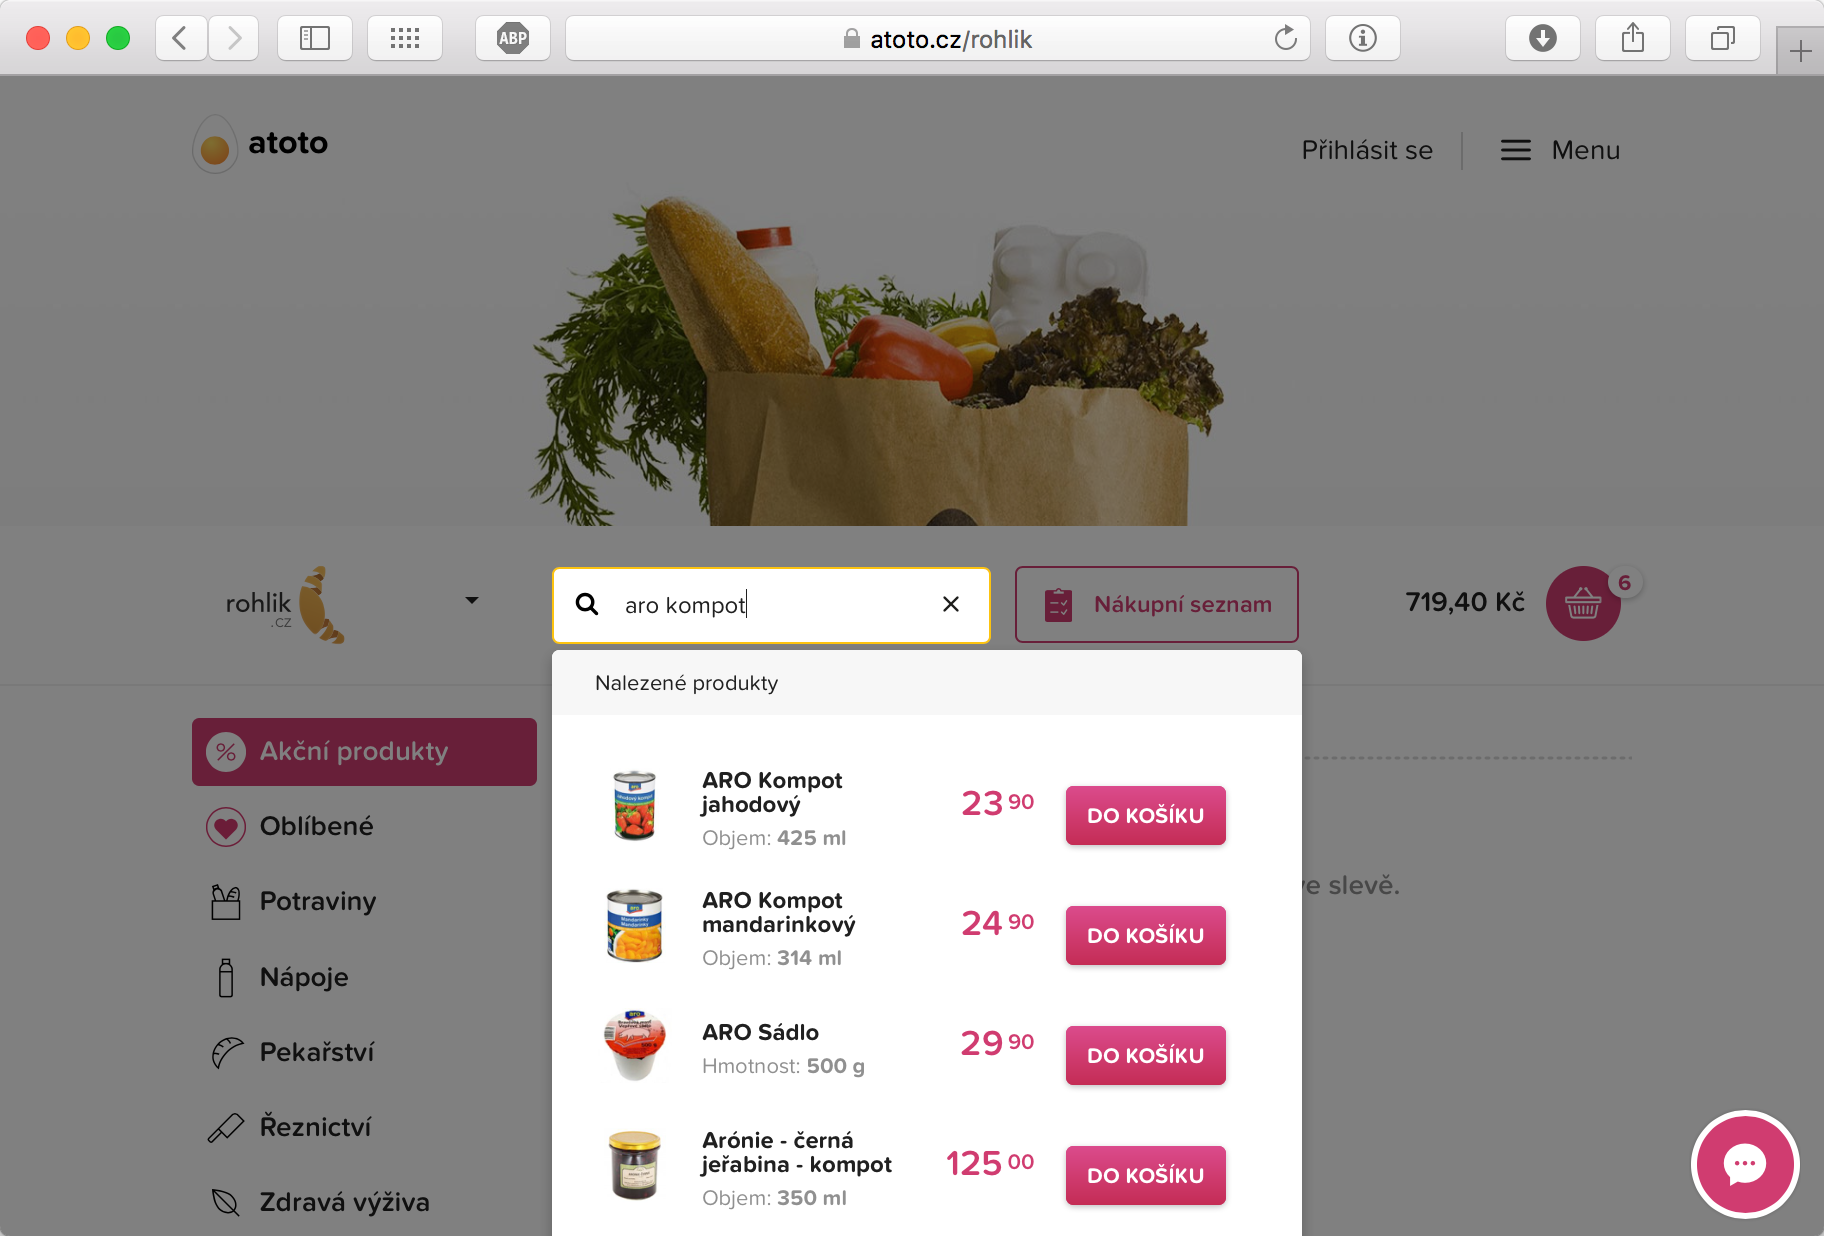
\includegraphics[width=\textwidth]{atoto-vyhledavani.png}
\caption[Ukázka plnotextového vyhledávání]{Ukázka plnotextového vyhledávání v elektronickém obchodu atoto.cz}
\label{atoto-vyhledavani}
\end{figure}

Implementace plnotextového vyhledávání však není triviální záležitostí. Vstup uživatele
je v přirozeném jazyce, takže je třeba jej odpovídajícím způsobem zpracovat, 
aby bylo vůbec vyhledávání na webu použitelné. Studium této problematiky
může být zdlouhavé a v konečném důsledku drahé. Je třeba brát v potaz
i případnou složitost dalších nástrojů, které bude třeba pro funkční vyhledávání spravovat, 
to s sebou nese více prostoru k potenciálním chybám.

Pokud bude k dispozici hotové řešení, které bude snadno nasaditelné na elektronický obchod 
a bude umožňovat jednoduché uzpůsobení potřebám konkrétního webu, bude to výrazná úspora jak 
času, tak peněz provozovatele elektronického obchodu.

Veškeré výše jmenované problémy mohou být značnou bariérou pro implementaci kvalitního vyhledávání, 
přes kterou se tak množství zejména menších obchodů nepřenese. Problémy lze shrnout do následujících bodů:

\begin{itemize}
\item Provozovatel elektronického obchodu chce nasadit textové vyhledávání na web, to se musí naprogramovat
\item Aktuální podoba textového vyhledávání na webu je nekvalitní
\item Vyhledávání na webu je pomalé, s přibývajícími produkty stále hůře použitelné
\end{itemize}

Řešení vyhledávání svépomocí je navíc z teoretického hlediska obtížné z~těchto důvodů:

\begin{itemize}
\item Je nutná znalost principů přirozeného jazyka
\item Je nutná znalost nástrojů, které umožňují pokročilou práci s jazykem
\item Je nutná znalost technologií, které poskytnou vyhledávání dostatečně rychlé
\end{itemize}

\section{Specifika elektronického obchodování}

V prostředí elektronického obchodování existují jisté vzorce, které se opakují a odlišují
toto prostředí od ostatních. Vyhledávají se zpravidla produkty (případně služby), které jsou
zařazeny do určitých kategorií a disponují atributy jako cena, název, kód, popis, url, obrázek, 
dostupnost a dalšími parametry, které bývají číselné (hmotnost, objem) nebo výčtové (barva, značka). 

Z toho vyplývá co a podle čeho se bude vyhledávat. Produkty mívají jednoznačné identifikátory, 
které jsou navíc standardizovány (EAN, ISBN). Pomocí těchto kódů je možné vyhledat produkty
napříč elektronickými obchody nebo je párovat v cenových srovnávačích. Pro vyhledávání
je však nejdůležitější název produktu, případně jeho varianta, která upřesňuje konkrétní
verzi produktu. Méně častěji je nutné vyhledávat v popisu produktu, kde bývá uveden
jak slovní popis, tak výpis parametrů. 

U produktů dále bývá evidována cena, která může být interně uložena v kombinaci s marží.
Obchody operující se zlevněným zbožím pak mívají uvedenou cenu jak před slevou, tak po této
slevě, aby zákazník viděl, kolikaprocentní sleva je na produktu. I samotná cena produktu
(případně marže prodejce) může hrát svou roli ve vyhledávání.

\section{Definice požadavků na vyhledávání} \label{ch:pozadavky-vyhledavani}

Požadavky na samotné vyhledávání jsou ovlivněny prostředím, ve kterém vyhledávání
probíhá a uživateli, kteří vyhledávání využívají. Primárně by mělo být možné
nalézt daný produkt podle jeho názvu, nebo části názvu, případně podle kódu produktu,
pokud je k~dispozici. Produkt by měl být ale vyhledatelný i podle dalších atributů, 
jako je název kategorie nebo název značky výrobce. Někdy dokonce uživatel nemusí
vyhledávat konkrétní produkt, ale jen produkty dané značky nebo kategorie, což by
měl systém také umět rozpoznat.

Podoba vyhledávaných výrazů bude zadávána zákazníky v přirozeném jazyce, s čímž by si mělo
vyhledávání také poradit. Konkrétně jde o tvarosloví, kdy může uživatel zadat výraz
například v jiném pádu, než je uvedeno v názvu produktu. Dále jde o vyrovnání se
s~chybami, které mohou vzniknout při formulaci vyhledávaného výrazu -- překlepy nebo
pravopisné chyby. V neposlední řadě jde také o vztah slova k jeho významu, kdy může
jedno slovo mít více významů (homonymum) nebo naopak více slov může odpovídat jednomu výrazu
(synonymum).

Další problematikou při zadávání hledaného výrazu uživatelem, je poskytování relevantních výsledků
už ve chvíli, kdy uživatel formuluje dotaz, tedy jej teprve píše. V takovém případě je třeba
odhadnout, který výraz chce napsat a tuto informaci využít při zobrazení odpovídajících
výsledků.

Ve chvíli, kdy systém zná produkty, které odpovídají hledanému výrazu by měl
výsledky poskytovat ve vhodném pořadí, měl by tedy pracovat s relevancí výsledků vzhledem 
k~zadanému výrazu. Toto může být velmi obtížné, protože každý uživatel má zájem o jiné
produkty a tak pro něj mohou být pro jeden výraz relevantní jiné produkty, než pro někoho
jiného. Dále do tohoto pořadí mohou vstupovat požadavky provozovatele elektronického obchodu
v případě, kdy má specifické požadavky na zboží, které chce nabízet přednostně. Důvodů
pro takové chování může být více, může souviset s marží konkrétních produktů, 
nebo s filozofií samotného obchodu. Tato problematika je však značně rozsáhlá a vydala by
na samostatnou práci, v tomto okamžiku je tedy nutné využít "objektivní" relevance, 
tedy řadit produkty pouze dle jejich podobnosti vzhledem k hledanému výrazu.

\section{Technické požadavky na aplikaci}

Na aplikaci je kladeno několik technických požadavků. Nejedná se o funkční požadavky, nýbrž
o požadavky související s použitelností, výkonností, spolehlivostí a podporou. Naplnění těchto
požadavků zajistí následný bezproblémový chod aplikace a uspokojení potřeb zákazníka.

Prvním technickým požadavkem na aplikaci je její rychlost. Ta je důležitá pro spokojenost
koncového zákazníka, který provádí vyhledávání. Všechny části aplikace nejsou z hlediska rychlosti
tak kritické, jedná se primárně o samotné vyhledávání. Akceptovatelná rychlost uživatelského rozhraní 
v tomto případě je 100 ms \cite{amazon-100ms}, v ideálním případě do 50 ms \cite{stackshare-algolia}. 
Pro naplnění tohoto požadavku je třeba, aby byla rychlost odezvy API co nejnižší.
Rychlost by dále nemělo výrazně ovlivňovat množství současných požadavků. 
Aplikace by měla být navržena tak, aby ji bylo možné snadno škálovat při zvyšující se zátěži.

Dalším požadavkem je formát samotného API. Bude třeba použít takový formát, který bude
co nejsnadněji implementovaný v používaných webových technologiích pokud možno bez instalace
jakýchkoli rozšíření. To je důležité pro rychlé nasazení aplikace do provozu a odbourání
možných vstupních bariér při rozhodování o využití nástroje. Pro načtení produktů
z elektronických obchodů by bylo ideální využít stávajících exportů pro jiné systémy, 
kterými by obchody mohly implementovat. Pokud by nic takového neexistovalo, můsí být vytvoření
exportu produktů pro provozovatele elektronického obchodu co nejsnažší.

Posledním technickým požadavkem je dokukemantace samotného API. Dokumentace musí být
dobře pochopitelná, tedy psaná přehledně, ideálně s konkrétními ukázkami použití.
Výhodou je také možnost vyzkoušet si práci s API vůči testovacímu prostředí, 
kde nehrozí riziko vzniku chyb na produkčních datech.

\section{Popis oborů, kterých se práce dotýká}

Samotné řešení problematiky vyhledávání je výrazně interdisciplinární obor. Je nutné
mít značné povědomí o získávání informací, počítačovém zpracování přirozeného jazyka, 
což souvisí jak s počítačovou lingvistikou, tak úzce s teorií formálních jazyků a překladačů.
Existuje také vztah mezi lingvistikou a logikou, jakožto vědě o myšlení, která se odehrává 
v kategoriích lidského jazyka. Podobný vztah lze nalézt také s umělou inteligencí, 
vzhledem k tomu, že používání přirozeného jazyka je inteligentní činností.
Díky tomu, že probíhá ukládání dat, je důležitá znalost teorie datových modelů.
Vzhledem k množství ukládaných dat se také můžeme dotýkat oboru Big Data.
V neposlední řadě je třeba porozumnět potřebám potenciálních uživatelů, tedy mít
určitou znalost podnikání a obchodování.

\section{Stávající možnosti implementace vyhledávání}

Na trhu existuje několik služeb, které umožňují implementaci plnotextového vyhledávání.
Ty se však liší funkčností, obtížností implementace i cenou. Níže popisuji nejvýznamější 
z nich zejména vzhledem k požadavkům na aplikaci.

\subsection{Využití relační databáze}

První možností, jak vyhledávání implementovat je využití stávající databáze, 
kterou elektronický obchod disponuje. Ať už se jedná o open source (MySQL, Postgres)
nebo komerční (SQL Server, Oracle) databázi, možnosti plnotextového vyhledávání
jsou zde omezené. Výhodou je to, že jsou data stále v jednom úložišti, není třeba
řešit správu (instalaci, konfiguraci nebo zálohování) dalšího nástroje. Ani vývojáři 
se nemusí učit nic nového, pouze využijí stávající databázi. Vyhledávání zde probíhá
v nejjednodušší formě pomocí operátoru \verb|LIKE|. Některé databázové systémy
disponují pokročilejšími funkcemi, kterými lze vyhledávání zlepšit \cite{postgres}.

\subsection{Elasticsearch, Apache Solr, Sphinx Search}

Využitím nástrojů přímo určených pro implementaci plnotextového vyhledávání lze 
dosáhnout nejlepších výsledků, ať už se jedná o Elasticseacrch či Apache Solr využívající
Apache Lucene \cite{lucene}, nebo Sphinx. Jde o typický krok v okamžiku, kdy
přestává funkčnost relační databáze pro potřeby vyhledávání dostačovat. Tyto nástroje
umožňují pokročilé nastavení indexace a zároveň jsou dostatečně rychlé, aby byly
schopny provádět vyhledávání v řádu milisekund. Výhodou je i cena -- zde uvedené nástroje
jsou poskytovány zdarma, placená bývá až možnost využití podpory nebo rozšiřujících funkcí.
Zřejmou nevýhodou tohoto řešení je nutnost znalosti dalšího nástroje, jeho správa a řešení 
synchronizace se stávající databází.

\subsection{Algolia}

Algolia je pokročilý nástroj umožňující imlementaci plnotextového vyhledávání \cite{algolia}. 
Zaměřuje se na poskytování kvalitních výsledků v co nejkratším možném čase (v řádu milisekund). 
Snaží se usnadnit práci programátorům tím, že nabízí řadu připravených integrací 
pro konkrétní programovací jazyky a frameworky. Kromě výsledků vyhledávání umožňuje 
faceting, tedy dodání dat pro tvorbu filtrů, podporuje řadu jazyků nebo vyhledávání 
podle geografické lokality. V neposlední řadě je k dispozici dashboard zobrazující 
stav systému a statistiky vyhledávání.

Pokud si zákazník vystačí s 10 000 vyhledatelnými produkty, může nástroj Algolia používat
zdarma, pouze je povinnen uvést ve výsledcích vyhledávání logo firmy. Placené verze 
začínají na 59 dolarech za měsíc za 100 000 produktů.

\subsection{Swiftype Site Search}

Swiftype Site Search je nástroj podobný nástroji Algolia, zaměřuje se však více na 
uživatelské rohraní a celkově na snadnost použití \cite{swiftype}. Mezi jeho hlavní
funkce patří vyhledávání v okamžiku formulace hledaného výrazu, možnost filtrace
výsledků, dodatečná úprava pořadí výsledků ručním zásahem na úrovni konkrétních 
výsledků, nebo na základě některého z atributů produktu. V nesposlední řadě je také
k dispozici přehledná analytika proběhlého vyhledávání. Cena za provoz služby
je od 299 USD měsíčně.

\subsection{AWS CloudSearch}

Firma Amazon poskytuje v rámci svého cloudu službu CloudSearch \cite{cloud-search}.
Jejími přednostmi jsou především vysoká výkonnost a škálovatelnost. Velkou vstupní
bariérou je však její počáteční složitost. Uživatel musí nejprve proniknout do 
některých základních konceptů Amazon Web Services, až poté může začít pracovat
se samotným vyhledáváním. Co se funkčnosti týče, nabízí služba podporu 34 jazyků, 
možnost nastavení váhy jednotlivých atributů, nebo doplňování texu během psaní.
Cena záleží na využití výpočetní kapacity, její určení je tedy složitější.

\subsection{Google Custom Search Engine}

Google Custom Search Engine \cite{gse} se nejvíc odlišuje od ostatních služeb. 
Vyhledávání je plně řízeno algoritmem společnosti Google a také výsledky vyhledávání
vypadají obdobně jako výsledky vyhledávání na www.google.com. 
Odlišné je i samotné napojení na službu -- výsledky vyhledávání jsou na web
vloženy jako samostatná stránka, na které je vidět logo společnosti Google.
Základní varianta je však zdarma, je to tedy levná cesta, jak rychle zprovoznit
vyhledávání na webu. Pokročilejší varianta umožňující konfiguraci stojí 100 USD ročně.

\section{Odůvodnění vytváření nového nástroje}

Výše uvedené nástroje sice umožňují implementaci textového vyhledávání, lze s nimi
dosáhnout dobrých výsledků. Nicméně pokud provozovatel obchodu není ochoten investovat
velké částky do pokročilých řešení, nastává problém. Tento problém je ještě výraznější, 
pokud obchod nedisponuje vlastním IT oddělením a pro samotnou implementaci vyhledávání
je vhodné využít minimum času najímaných IT specialistů.

Vzhledem k zjištěným problémům při implementaci textového vyhledávání je očekávaným
přínosem této práce, respektive vzniklé aplikace:

\begin{itemize}
\item Na webu obchodu bude dříve kvalitnější a rychlejší vyhledávání
\item Ryhlejší implementace vyhledávání (pokud ještě na webu žádné není)
\item Vyhledávání může být outsourcováno (úspora nákladů na IT i provoz)
\end{itemize}


%%%%%%%%%%%%%%%%%%%%%%%%%%%%
\chapter{Plnotextové vyhledávání}

Tato kapitola popisuje problematiku textového vyhledávání a poukazuje tak na konkrétní
problémy, které je při vyhledávání nutno řešit. Problematika je rozebírána v kontextu
elektronického obchodování, jsou tedy uváděny pouze principy aplikovatelné v tomto
oboru.

Vyhledávání je proces sestávající jednak z ukládání dokumentů určených k~vyhledávání
a dále z provedení vyhledávání uživatelem. Obecné schéma vyhledávání vypadá následovně:

\begin{figure}[h]
\center
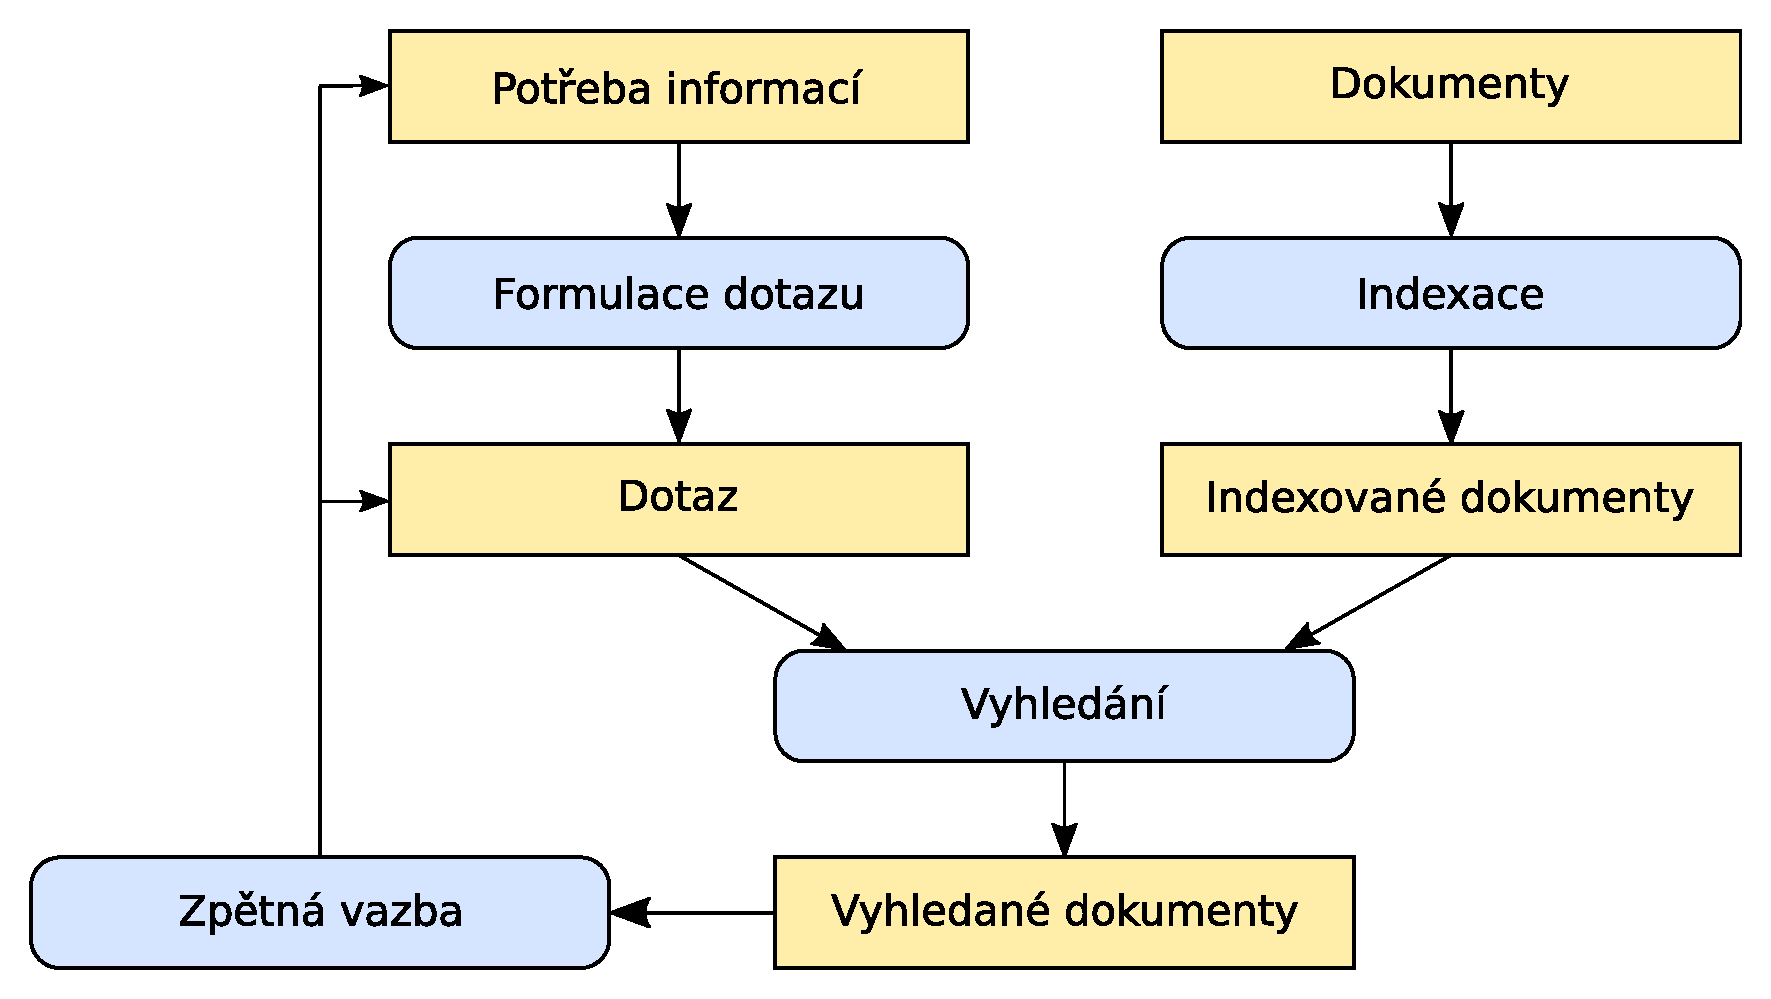
\includegraphics[width=\textwidth]{schema-vyhledavani.pdf}
\caption[Proces vyhledávání]{Proces vyhledávání (Zdroj: \cite{searching})}
\label{schema-vyhledavani}
\end{figure}

Ukládání dokumentů probíhá tak, že se upraví pro potřeby vyhledávání a uloží 
do indexu, přičemž celý tento proces se označuje jako indexace. Ve chvíli, kdy jsou
dokumenty připraveny k vyhledávání, může uživatel mající potřebu v těchto dokumentech 
vyhledávat (získávat z nich informace) formulovat dotaz, kterým chce získat odpovídající
dokumenty. Z něj je vytvořen dotaz, podle nějž bude vyhledávání provedeno. Následně
jsou uživateli dodány dokumenty vyhovující dotazu, ten pak může dotaz na základě
získaných dokumentů a pochopení způsobu vyhledávání dotaz upravit.

\section{Analýza dat, v kterých bude vyhledáváno}

Nejprve je třeba prozkoumat data, ve kterých bude vyhledávání prováděno. Vycházím
ze~skutečnosti, že naprostá většina elektronických obchodů své zboží nabízí také 
prostřednictvím srovnávačů zboží, přičemž v počtu návštěv a tedy celkovém provozu 
v~rámci českého internetu jsou nejdůležitější Heureka.cz a Zboží.cz \cite{netmonitor}. 

Data pro tyto srovnávače musí být dodávána prostředníctvím XML feedu, který odpovídá 
specifikaci jednotlivých systémů. Při porovnání obou specifikací lze nalézt 
jistou podobnost v požadovaných údajích. Samotný XML feed obsahuje
produkty obchodu, přičemž u každého produktu je možné uvést několik atributů, z~nichž
některé jsou povinné. Konkrétně v případě Zboží.cz musí mít každý produkt uveden název, 
popis, URL, cenu a dostupnost. Dále lze využít volitelných parametrů jako název kategorie, 
název značky a výrobce, EAN, ISBN, produktový kód výrobce, případně další doplňkové
informace a parametry \cite{xml-zbozi}. V případě Heuréka.cz je podstatný název
obsahující případně výrobce a produktové číslo či kód, název kategorie, dostupnost a
cena dopravy. Informace o produktu mohou dále obsahovat popis, EAN, kód produktu
nebo soupis parametrů \cite{xml-heureka}. Minimální XML soubor s jedním produktem 
ve formátu Heuréka je zobrazen ve výpisu \ref{code:xml-heureka}.

\begin{code}
\captionsetup{singlelinecheck=false,justification=raggedright}
\captionof{listing}{Ukázka XML souboru ve formátu Heuréka.cz}
\label{code:xml-heureka}
\begin{minted}{xml}
<?xml version="1.0" encoding="UTF-8"?>
<SHOP>
 <SHOPITEM>
  <ITEM_ID>40272131</ITEM_ID>
  <PRODUCT>
   Matrace MYRBACKA - Latexová matrace, střední tvrdost, bílá
  </PRODUCT>
  <PRODUCTNAME>Matrace MYRBACKA</PRODUCTNAME>
  <DESCRIPTION>
   <![CDATA[Latex vám umožní lépe odpočívat a to tak, že sleduje
    kontury vašeho těla, uvolňuje tlak a poskytuje podporu.
     - Potah: 64% polyester, 36% bavlna
     - Vnitřní látka: Netkaný polypropylen, 100% jehněčí vlna
     - Komfortní materiál: syntetický latex, pěna polyuretan]]>
  </DESCRIPTION>
  <URL>http://ikea.com/cz/cs/catalog/products/40272</URL>
  <IMGURL>http://ikea.com/cz/cs/images/products/40272.JPG</IMGURL>
  <PRICE>9087</PRICE>
  <PRICE_VAT>10990</PRICE_VAT>
  <CATEGORYTEXT>Dům a nábytek | Nábytek | Matrace</CATEGORYTEXT>
  <MANUFACTURER>IKEA</MANUFACTURER>
 </SHOPITEM>
</SHOP>
\end{minted}
\end{code}

Na základě znalosti struktury XML souboru lze zjistit, že při využití stávajících exportů
internetových obchodů bude každý produkt obsahovat název, popis, URL, cenu, dostupnost
a název kategorie, přičemž pravděpodobně bude k dispozici řada dalších atributů, 
dle použitého formátu feedu a dle pečlivosti provozovatele obchodu.

\section{Automatické indexování textů} \label{ch:indexace}

Indexace je proces, kdy jsou ukládány textové dokumenty určené k vyhledání \cite[strana~15]{strossa}.
Ukládány jsou pouze výrazy, podle nichž by měl být ukládaný dokument vyhledatelný, 
místo kam jsou tyto výrazy ukládány se nazývá index. Jedná se vlastně o klíče, 
podle kterých bude bude možné rychle hledaný záznam nalézt. To je důležité z hlediska
rychlosti vyhledávání -- není možné všechny uložené záznamy procházet a analyzovat
až ve chvíli vyhledávání. 

Při indexování je třeba analyzovat každý výraz, který by měl být uložen do indexu.
V prvé řadě je třeba rozhodnout, zda je třeba jej do indexu ukládat, je tedy 
třeba řešit významnost jednotlivých výrazů v textu. Pokud daný
výraz není pro vyhledávání užitečný, nemá smysl jej ukládat. Dalším problémem je 
tvarosloví, tedy to, že slova mohou měnit tvar (jedná se například o skloňování 
podstatných jmen), stále se přitom jedná o jedno slovo. V neposlední řadě je také 
třeba zohlednit význam slov v daném oboru, kdy mohou stejná slova vyjadřovat jiné věci 
(homonymie -- například myš ve smyslu počítačového příslušenství a myš jako zvíře), 
nebo může být jeden význam vyjádřen různými slovy (synonymie -- lednička i chladnička 
označuje totéž). Konečně je také třeba brát v úvahu další vztahy mezi slovy, 
jako nadřazenost a podřazenost. Například banán a ovoce mohou označovat totéž, 
přičemž ovoce to činí v širším slova smyslu, toto označení lze použít i pro jiné 
ovoce, například jablko.

\section{Specifika českého jazyka}

Vzhledem k tomu, že je vyhledávání vytvářeno pro české internetové obchody, 
bude veškeré vyhledávání probíhat v českém jazyce, a proto nyní popíši jeho specifika.
Český jazyk pracuje se slovy odlišně než jiné jazyky. Dochází i k drobným
odchylkám i v rámci českého jazyka na základě geografické oblasti (nářečí)
nebo na základě zaměření dané skupiny lidí (hantýrka). Dále se můžeme zabývat
grafickou podobou jazyka (morfologií) nebo jeho zvukovou podobou (fonetikou).
Vzhledem k tomu, že vyhledávání probíhá na textové bázi, zabývám se dále právě 
grafickou podobou jazyka.

Slova jsou v českém jazyce řazena do slovních druhů, kterých je celkem deset.
Slovní druh pomáhá určit chování slova -- slova stejného slovního druhu se ohýbají
a vyskytují v textu podle podobných pravidel. Slovní druhy lze dělit podle
toho, zda jsou ohebné (tedy zda se jejich tvar může měnit) a neohebné.
Neohebné slovní druhy jsou zpravidla používány ve větě společně s obehnými, 
protože samy o sobě nenesou informační hodnotu. Naopak ohebné slovní druhy
samy o sobě nesou informační hodnotu, jsou proto vhodnými kandidáty pro
to, aby se podle nich vyhledávalo. Výjimkou jsou zde zájmena, která nesou 
informaci nepřímo.

\begin{figure}[h]
\center
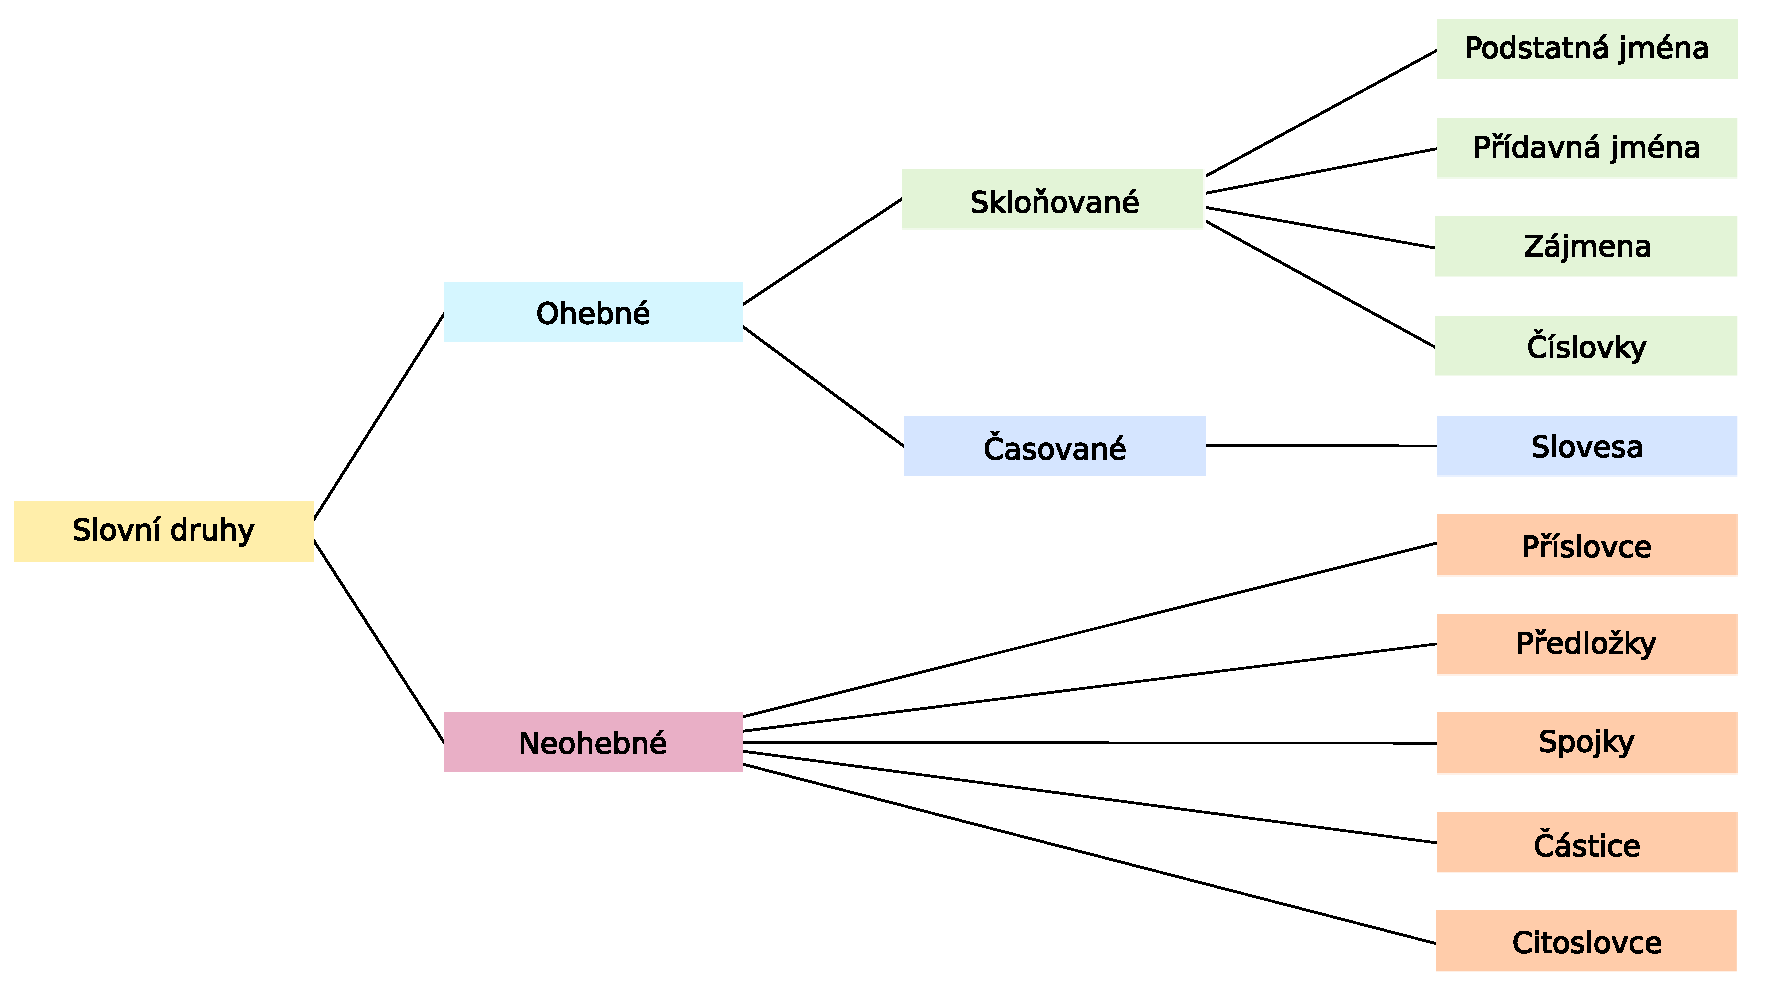
\includegraphics[width=\textwidth]{slovni-druhy.pdf}
\caption{Dělění slovních druhů dle jejich ohebnosti}
\label{slovni-druhy}
\end{figure}

V rámci ohebnosti lze rozlišovat jakým způsobem jsou ohýbána. Slovesa mohou být
časována, příslovce mohou být stupňována, podstatná jména, přídavná jména, zájmena
a číslovky mohou být skloňována. Dále v češtině rozlišujeme tři jmenné rody
(mužský, ženský a střední) a dvě čísla (jednotné a množné). U sloves navíc 
rozlišujeme jejich vid.

\section{Problematika tvarosloví}

První problém související s zpracováním přirozeného jazyka je vypořádání se s tvaroslovím
(morfologií). Jednotlivá slova se v českých textech objevují v různých slovních tvarech, 
málokdy jsou všechna slova v základním tvaru. Například jeden produkt může mít název
\textbf{Alex Čistič na laminát s pomerančovým olejem} i \textbf{Alex čistič na laminát pomerančový olej}.
V obou případech je uveden \textbf{pomeranč}, jen v různém tvaru. Při vyhledávání je však
žádoucí docílit toho, aby byla obě slova vyhledatelná shodně, ať už bude slovo pomeranč
zadáno v kterémkoli pádě. Typické řešení je vřazení modulu do procesu indexace dokumentů nebo 
dotazů, který sjednocuje podobu porovnávaných slov.

\subsection{Základní pojmy tvarosloví}

V této části jsou vysvětlovány základní pojmy rozebíraného oboru. Jejich znalost je nutná k pochopení 
následujícího textu. Podrobnější popis těchto termínů lze nalézt v literatuře \cite{strossa}.

\subsubsection*{Morfém}

Morfém je minimální funkční jednotka s vlastním významem. Jde o základní jednotku vědy, 
která se zabývá tvorbou slov, tedy morfologie.

\subsubsection*{Lexém}

Lexém je základní stavební jednotka slovníku, znaková jednotka vyjadřující pojem nesoucí
význam. Je to základní jednotka vědy zabývající se slovní zásobou -- lexikologie. Ta je stejně 
jako morfologie odvětvím lingvistiky. Každý lexém je pak možné dále dělit na koncovku, 
kmen, kořen, prefix a sufix.

\subsubsection*{Foném}

Foném je hláska umožňující rozlišit význam. Obory, pod které spadá, se zabývají zvukovou
stránkou jazyka a nazývají se fonetika a fonologie.

\subsubsection*{Flexe}

Flexe neboli ohýbání popisuje změnu slov vzniklou při skloňování, časování nebo ohýbání.
Jde o grafickou změnu lexému pro vyjádření odpovídajícího pádu, rodu a dalších gramtických
kategorií.

\subsection{Operátor pravostranného rozšíření}

Nejjednodušším řešením problematiky ohýbání slov je operátor pravostranného rozšíření.
Mějme slovo \textbf{svíčka}, které se při skloňování v jednotném čísle mění na svíčky, svíčce, 
svíčku, svíčko, svíčce, svíčkou. V tomto příkladu lze vypozorovat, že se mění
pouze konec slova, zatímco levá část \textbf{svíč-} zůstává stejná. Tento přístup bude 
sice poměrně úspěšný, nicméně se nevyhneme případům, kdy bude mít více slov stejný
základní tvar. Mohli bychom tak při vyhledání výrazu \textbf{svíčk} obdržet i dokumenty
obsahující slovo \textbf{svíčková}.

Vzhledem k jednoduchosti a zároveň poměrně vysoké úspěšnosti bývá tento přístup
často využíván jako jedna z prvních implementací plnotextového vyhledávání přímo
v relační databázi pomocí operátoru \verb|LIKE|. Konkrétně vyhledávání v jazyce SQL
výše diskutovaného výrazu by bylo provedeno jako \verb|LIKE 'pomeranč%'|.

Kromě problému s možným shodným základem pro různá slova je další komplikací při 
použití této metody skutečnost, že při ohýbání slov nedochází pouze ke změně koncovek, 
ale často se mění také některá písmena základu slova. Uvažujme slovo \textbf{kůň}, které
má v~druhém pádu podobu \textbf{koně}. Pro tento případ by bylo možné rozšířit možnost 
pravostranného rozšíření o nahrazení pouze jednoho znaku. Pokud bychom tak měli 
pro nahrazení více písmen využít znak \textbf{*} a pro nahrazení právě jednoho písmene 
znak \textbf{?}, byl by základní tvar tohoto slova \textbf{k?ň*}. To je ale problém, protože 
takový výraz odpovídá například i slovu \textbf{kaňka}.

\subsection{Derivátor slovních tvarů}

Derivátor slovních tvarů je nástroj, který namísto daného slova vygeneruje 
všechny jeho gramatické tvary, případně jeho použitelné odvozeniny. 
Ty jsou následně použity jako jejich logická disjunkce. Například místo 
slova \verb|svíčka| by se použilo:

\begin{figure}[thp]
\centering 
\begin{minipage}{0.73\textwidth}
\begin{minted}{bash}
(svíčky OR svíčce OR svíčku OR svíčko OR svíčkou 
  OR svíček OR svíčkám OR svíčkami OR svíčkách)
\end{minted}
\end{minipage}
\end{figure}

Takový nástroj musí obsahovat co nejpřesnější sadu pravidel, jak vytvářet
veškeré tvary zadaného slova. Dále je třeba k expandovanému slovu zadat
jeho veškeré informace, aby mohlo být vybráno správné pravidlo.

\subsection{Stematizace}

Stematizace je proces, kdy je slovo převáděno na jeho kmen (stem). Toho je docíleno
odstraněním předpon, přípon a koncovek. Její použití je vhodné pro jazyky, 
které mění slova jen tímto způsobem (např. Angličtina). Pro češtinu je však stematizace
hůře aplikovatelná, protože se slova ohýbají podle složitějších pravidel, ne jen
změnou předpon, přípon nebo koncovek. Stematizaci tedy lze využít při hledání základního
tvaru slova i v českém jazyce, je ale nutné ji rozšířit o další procesy, které jsou 
popisovány dále.

\subsection{Lematizace}

Lematizátor je nástroj, který převádí slovo na jeho základní gramatický tvar, tzv. lemma.
Základním gramatickým tvarem se rozumí první pád jednotného čísla u podstatných jmen nebo infnitiv 
u sloves. Celý proces se nazývá lematizace a kromě převodu na základní tvar může lematizátor
disponovat doplňkovou funkcí, kdy pro daný tvar poskytne i jeho vlastnosti, například 
slovní druh, pád nebo číslo. Lematizátor pracuje v podstatě opačně ve srovnání s derivátorem. 
Lematizace zároveň není totéž co stematizace, které předpokládá, že dochází 
jen k přidávání předpon a přípon. Lematizátor jej vlastně rozšiřuje, odstranění
předpon nebo přípon však může být jednou z jeho činností. Především ale počítá s~tím, 
že se koncovky nebo kmeny slov mohou měnit, což je důležité pro češtinu.
Dalším rozdílem je výsledek daného procesu -- po stematizaci může vzniknout díky ořezání
předpon a přípon neexistující slovo, výstupem lematizace je však vždy slovo existující.

Algoritmů pro implementaci lematizátoru je více, triviálním řešením může být použití
slovníku, který obsahuje veškerou slovní zásobu daného jazyka a všechny tvary těchto
slov. V něm je pak nalezeno slovo v daném tvaru a k němu odpovídající základní tvar.
Výhodou takového přístupu je přesnost lematizace, pokud je již daný tvar slova znám, 
je triviální najít přesný základní tvar. Jediný problém může způsobit duplicita daného 
slova, kdy se musí lematizátor rozhodnout, na který základní tvar jej upraví. Nevýhodou
je poté nutnost vytvoření takového slovníku, kdy je třeba popsat veškerou slovní zásobu.

Další možností je algoritmická lematizace, kdy jsou definována pravidla, podle kterých jsou
slova ohýbána, a ta jsou používána pro hledání základního tvaru. Využití takového přístupu
znamená daleko menší soubor pravidel, podle kterých je lematizace prováděna ve srovnání 
s~kompletním slovníkem slovní zásoby. Je tedy rychlejší takový lematizátor vybudovat
od počátku a ve srovnání s použitím slovníku je velká šance, že bude správně zpracováno
neznámé slovo. Pokud chybí ve slovníku, nelze rozhodnout, jak lema vytvořit. Pokud
však budeme mít definovánu jen sadu pravidel, spíše bude lematizace provedena úspěšně.
Zřejmou nevýhodou ve srovnání s využitím slovníku je kvalita takové lematizace. 
Čeština je dosti nepravidelná a existuje mnoho výjimek, které se při ohýbání slov vyskytují.

Konečně lze také pro lematizaci využít stochastických metod, respektive metod strojového
učení. Ručně se vytvoří trénovací data, která se následně použijí pro vytvoření modelu.
Na základě tohoto modelu lze provádět samotnou lematizaci, přičemž použitelných metod 
strojového učení je celá řada.

\section{Problematika významnosti}

Další problém, který je třeba řešit, je významnost výrazů, podle nichž je vyhledáváno.
Ne všechna slova jsou pro vyhledávání využitelná, protože nenesou žádnou užitečnou 
hodnotu, nebo jsou tak častá, že je jejich využití degradováno. 

Zároveň však ne všechna slova charakterizují daný dokument stejnou mírou. Nelze se tedy 
jen rozhodovat, zda dané slovo ukládat do invertovaného indexu, je také třeba pamatovat
na rozdílnou informační hodnotu slov vůči dokumentům -- ať už se jedná o indexovaný
dokument, nebo o celou jejich sadu.

\subsection{Negativní slovník}

Negativní slovník, někdy označovaný také jako stop-slovník nebo slovník stop-slov, 
je datová struktura obsahující slova, která jsou v daném případě považována za bezvýznamná
z pohledu vyhledávání. Bývají to slova určitých slovních druhů, nebo obecně slova, která 
nenesou žádný význam. Obvykle jde o předložky, spojky nebo zájmena. Někdy také může jít 
o~podstatná jména, která se v~dané oblasti vyskytují tak často, že jsou pro vyhledávání nepoužitelná.

Kromě výše uvedených slovních druhů by také bylo možné použít některá nejčastěji používaná
slova v českém jazyce \cite{nejpouzivanejsi-slova} . Pokud se podíváme na prvních 5 nejpoužívanějších 
přídavných jmen (jiný, určitý, další, nový, velký), zjistíme, že právě toto jsou slova, 
která pravděpodobně nepůjdou pro vyhledávání dobře použít. Pro vytvoření negativního slovníku 
tak bude potřeba existující slovník obsahující slova potřebných slovních druhů a některá tato 
nejpoužívanější slova.

Další možností, která může jednoduše vyloučit spojky a předložky, je odfiltrování krátkých
slov. Vzhledem k tomu, že většina takových slov má dělku jeden až dva, nejvýše tři znaky, 
je možné to v filtru zohlednit. Hlavní výhodou tohoto přístupu je rychlost oproti vyhledávání
slova v slovníku. Je tedy optimální oba přístupy kombinovat, nejprve odfiltrovat krátká slova
a poté využít slovníku stop-slov, která se tím výrazně zmenší (je možné krátká slova vypustit)
a celá indexace se tím zrychlí.

\subsection{Významnost výrazů}

Důležitá veličina při indexaci výrazu je jeho významnost, neboli míra reprezentace indexovaného
dokumentu. Některé výrazy totiž vystihují daný dokument přesněji než jiné. Uvažujme produkt
s názvem \textbf{Jablko Idared červené}. Slovo \textbf{Jablko} tento produkt vyjadřuje poměrně dobře, 
ale stále ještě příliš obecně. Pokud uživatel vyhledává podle tohoto výrazu, stále ještě nelze 
rozhodnout, že je tento produkt ten, který hledal. Slovo \textbf{Idared} již reprezentuje konkrétní
produkt daleko přesněji, žádný jiný produkt se takto pravděpodobně nejmenuje. Opakem je pak
slovo \textbf{červené}, které vystihuje produkt nejméně, červené mohou být i jiné potraviny (rajčata)
nebo dokonce úplně jiné produkty (například petrklíč červený). 

Z uvedeného příkladu lze vypozorovat, že významnost výrazu souvisí s jeho výskytem v celém
souboru indexovaných dokumentů. Přesněji jde o vztah mezi frekvencí výrazu (TF -- term frequency) 
a frekvencí v invertovaných dokumentech (IDF -- inverse document frequency) \cite[strana~21]{strossa}. 
Ty lze vypočítat pomocí vzorců:

\[tf(t,d) = 0.5 + 0.5 \cdot \frac{f_{t,d}}{max\{f_{{t}',d}:{t}'\in d\}}\]
\vspace{1mm}
\[idf(t,D)=log \frac{N}{\left | \{d\in D:t\in d\} \right |}\]
\vspace{1mm}

Samotná váha daného výrazu (TF-IDF) \label{tfidf} je definována jako součin těchto hodnot:

\vspace{1mm}
\[tfidf(t,d,D) = tf(t,d) \cdot idf(t,D)\]
\vspace{0mm}

Pro zpřesnění tohoto výpočtu je možné dále pracovat s váhou a to jak u frekvence výrazu, 
tak u frekvence v invertovaném indexu. Hodnoty bývají nejčastěji normalizovány nebo
logaritmovány.

\section{Tezaurus}

Tezaurus označuje slovník, který charakterizuje vztahy mezi slovy. Zachycuje podobnost, 
nadřazenost nebo podřazenost mezi slovy. Lze jej využít při indexaci nebo formulaci 
dotazu a s jeho pomocí je možné daná slova rozšířit o slova s obdobným významem, 
přičemž význam může být obecnější nebo naopak přesnější. Tezaurus je díky množství
vztahů které popisuje propracovanější než jen seznam synonym. Lze jej využít 
i pro neobvyklá slova, jako je žargón nebo další expresivní výrazy.

Vytvoření takového slovníku je závislé na oblasti, pro kterou je vytvářen. Například 
slovo \textbf{oko} bude nahraditelné jinými slovy v kontextu gastronomie a jinými 
slovy v oboru biologie. Nelze tedy bezmyšlenkovitě používat jeden takový slovník globálně 
pro veškeré vyhledávání, je třeba zohlednit obor, ve kterém bude využíván.

\section{Přibližné vyhledávání}

Dalším komplexním problémem, kterým je třeba se zabývat je přibližné vyhledávání, tedy
vyrovnání se s překlepy nebo schopnost vyhledat dokumenty už v okamžiku, kdy je formulován
vyhledávaný dotaz. Tato funkčnost je označována jako search-as-you-type nebo také
incremental search.

\begin{figure}[h]
\center
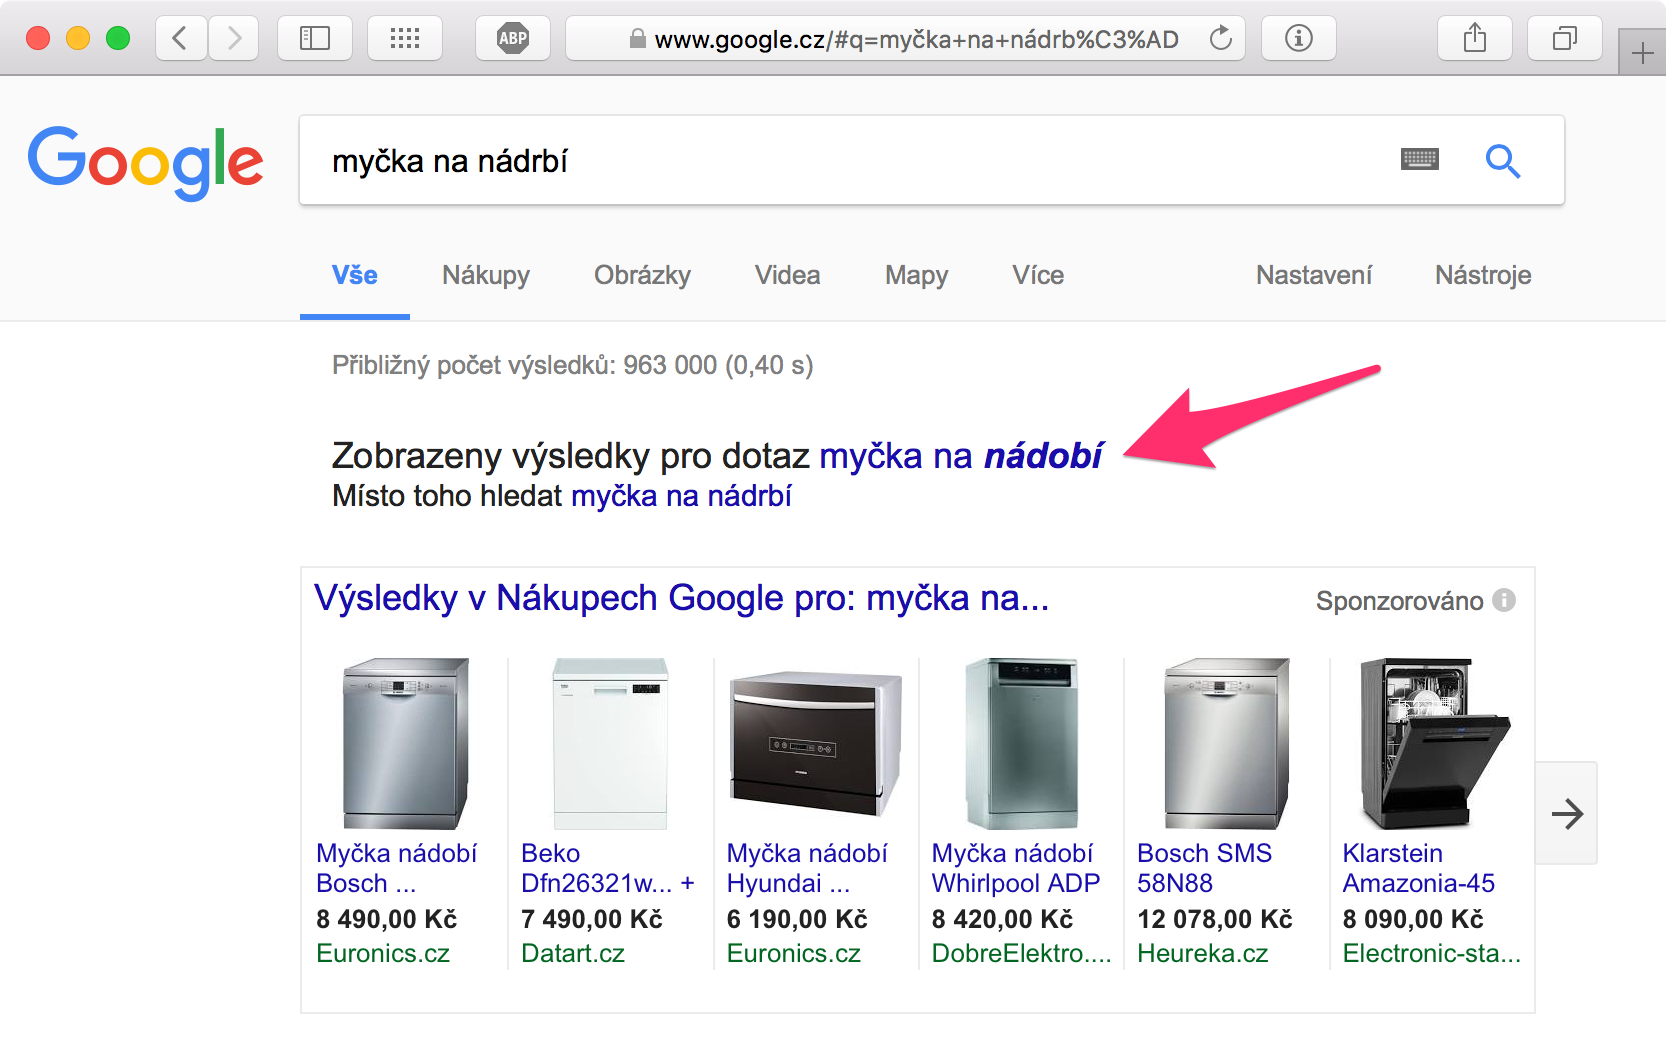
\includegraphics[width=\textwidth]{google-preklep.png}
\caption[Odhalení překlepu ve vyhledávání]{Odhalení překlepu ve vyhledávání na webu google.com}
\label{google-preklep}
\end{figure}

U přibližného vyhledávání je třeba se vypořádat s měrou, jak přibližný daný výraz
je vůči výryzu hledanému, což lze vyjádřit pomocí editační vzdálenosti. Přistoupit
k této problematice lze i jednoduším přístupem -- generováním n-gramů.

\subsection{Editační vzdálenost}

Editační vzdálenost je způsob, jak vyjádřit podobnost dvou textových řetězců. Je
vyjádřena jako celé číslo, které udává počet operací nutný pro transformaci z~jednoho
textového řetězce na druhý. Editačních vzdáleností pro textové vyhledávání je více, 
podle toho, jaké operace na textovém řetězci umožňují.

V roce 1965 Vladimir Levenshtein definoval \textbf{Levenshteinovu vzdálenost} jako počet
změn znaků vedoucí k transformaci z jednoho textu na druhý \cite{es-fuzziness}:

\begin{itemize}
\item Nahrazení jednoho znaku jiným: \textbf{jxblko} \textrightarrow ~\textbf{jablko}
\item Vložení jednoho znaku: \textbf{jaxblko} \textrightarrow ~\textbf{jablko}
\item Odstranění jednoho znaku: \textbf{jblko} \textrightarrow ~\textbf{jablko}
\end{itemize}

Frederick Damerau ji později rozšířil o další transformaci, která má shodnou váhu:

\begin{itemize}
\item Prohození dvou znaků: \textbf{jbalko} \textrightarrow ~\textbf{jablko}
\end{itemize}

Tato transformace vlastně nahrazuje více dílčích operací definovaných výše. 
Vzdálenost s touto transformací o hodnotě 1 je označována jako 
\textbf{Damerau–Levenshteinova vzdálenost}. 
Počtem transformací se zvyšuje editační vzdálenost a zároveň
s~ní se snižuje pravděpodobnost, že daný textový řetězec je překlepem
druhého řetězce. Damerau vypozoroval, že 80\% překlepů má editační vzdálenost 
rovnou jedné \cite{damerau}. Je tedy výrazně nižší pravděpodobnost, že 
v textu bude tolik chyb, aby byla vzdálenost vyšší, což lze zohlednit při konstrukci
vyhledávacího algoritmu a bude mít zřejmě pozitivní vliv na rychlost vyhledávání.

Další vzdáleností je \textbf{Hammingova vzdálenost}, která počítá pouze s náhradou
znaku v textovém řetězci. Z tohoto omezení je však patrné, že je použitelná pouze pro 
řetězce shodné délky. V praxi textového vyhledávání tedy budeme pracovat pravděpodobně
s~vzdálenostmi definovanými výše.

Na mírně odlišném principu funguje \textbf{vzdálenost nejdelšího společného podřetězce}
(nebo také posloupnosti -- LCS distance). Jejím úkolem je nalézt nejvyšší možný za sebou
jdoucí počet znaků, který je společný oběma řetězcům. Tento přístup je ale méně
chodný pro vyrovnání se s chybami uprostřed slov, navíc je výpočetně náročnější.

Další z možných vzdáleností je \textbf{Jarova vzdálenost}, která kromě počtu
změn na znacích počítá i počet shodných vzdáleností. Jejím rozšířením je
\textbf{Jaro-Winklerova vzdálenost}, která navíc počítá s~tím, že shodnost 
na~začátku řetězce má vyšší váhu, než na jeho konci -- vychází
totiž z pozorování, že na začátku textu se vyskytuje méně chyb \cite{christen}.
Tento přístup také dosahuje lepších výsledků u krátkých slov.

\subsection{N-gramová podobnost}

Vytváření n-gramů je používáno při indexaci, kdy jsou slova dělena na části dlouhé \verb|n| znaků.
Pokud bychom měli vygenerovat n-gramy o délce 3 (trigramy) pro slovo \textbf{telefon}, byly by 
to výrazy: \textbf{tel}, \textbf{ele}, \textbf{lef}, \textbf{efo} a \textbf{fon}. Lze si 
všimnout, že jednotlivé vygenerované výrazy se překrývají. Pokud pak uživatel zadá jako hledaný 
výraz \textbf{telef}, bude odpovídat trigrmům \textbf{tel}, \textbf{ele} a \textbf{lef}, 
tedy třem z celkem pěti. Trigramy jsou společně s digramy (n-gramy o délce dvou znaků) nejvhodnější
vzhledem k obvyklé délce slov. N-gram o délce 1 pak ztrácí smysl výše nastíněné logiky.

Porovnávání slov pomocí n-gramů je znázorněno na~následujícím schématu. Zde je zadané slovo
rozděleno na trigramy, z nichž každý je dále porovnávám s trigramy indexovaných slov.

\begin{figure}[h]
\center
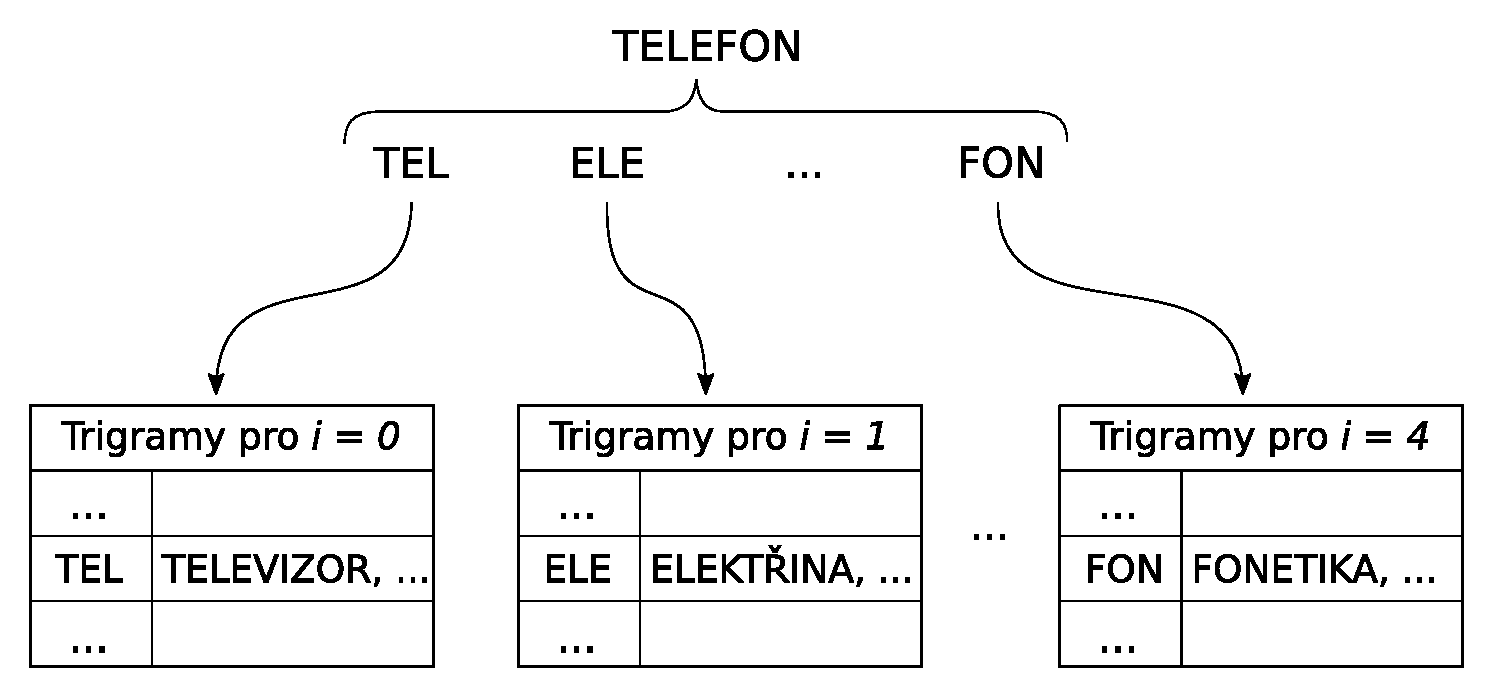
\includegraphics[width=\textwidth]{n-gram.pdf}
\caption[Vyhledávání pomocí n-gramů]{Vyhledávání pomocí n-gramů (Zdroj: \cite{n-gram})}
\label{n-gram}
\end{figure}

Tento mechanismus lze použít pro našeptávání i pro odhalení překlepů. Je snadno implementovatelný
a poměrně rychlý, selhává však u~překlepů v krátkých slovech~\cite{n-gram}. Předpokládejme slovo 
o~délce 5 znaků -- \textbf{mobil}. Vzniklé trigramy jsou \textbf{mob}, \textbf{obi}, \textbf{bil}.
Pokud uživatel vyhledá slovo s překlepem přesně uprostřed (\textbf{movil}), nebude nalezena
shoda v žádném trigramu. 

Řešením by mohlo být snížení počtu znaků v n-gramu, což může na druhou stranu mít negativní 
vliv na~rychlost. Možným kompromisem tak může být různá délka n-gramů, kdy by vznikly kratší
n.gram pro začátek a konec slov. Konkrétně pro slovo \textbf{mobil} by tak vznikly n-gramy 
\textbf{m}, \textbf{mo}, \textbf{mob}, \textbf{obi}, \textbf{bil}, \textbf{il}, \textbf{l}.

\section{Relevance}

Relevancí rozumíme míru, jakou odpovídá nalezený dokument zadanému dotazu.
Je použitelná pro řazení nalezených dokumentů, kdy jsou nejprve zobrazeny dokumenty
více odpovídající hledanému výrazu. Dále je možné se na základě relevance rozhodnout, 
zda ještě nalezený dokument hledanému výrazu odpovídá, zda je vůbec třeba jej zobrazit.

Relevance je do jisté míry subjektivní, protože každý zákazník vyhledává na webu
s~jiným očekáváním, přestože třeba vyhledává pomocí stejných výrazů. Objektivně lze však
relevanci vyjádřit pomocí TF-IDF, tedy frekvence nalezených výrazů vůči jejich frekvenci
v invertovaném indexu. 

V praxi elektronických obchodů však často do řazení
vstupují další veličiny, jako je cena produktu, skladovost nebo výše marže.
Pokud například uživatel vyhledá \textbf{iPhone}, může být žádoucí nejprve zobrazit
produkt \textbf{iPhone SE 64GB Vesmírně černý}, než jeho příslušenství, například
\textbf{Sportovní obal na iPhone SE} z důvodu několikanásobně vyšší marže na tomto produktu.

Elektronické obchody často také operují s akčním zbožím. Zejména v České republice je
obchodování se zlevněným zbožím populární, může tak být žádoucí zobrazit takové produkty
dříve, než produkty prodávané za standardní cenu.

\begin{figure}[h]
\center
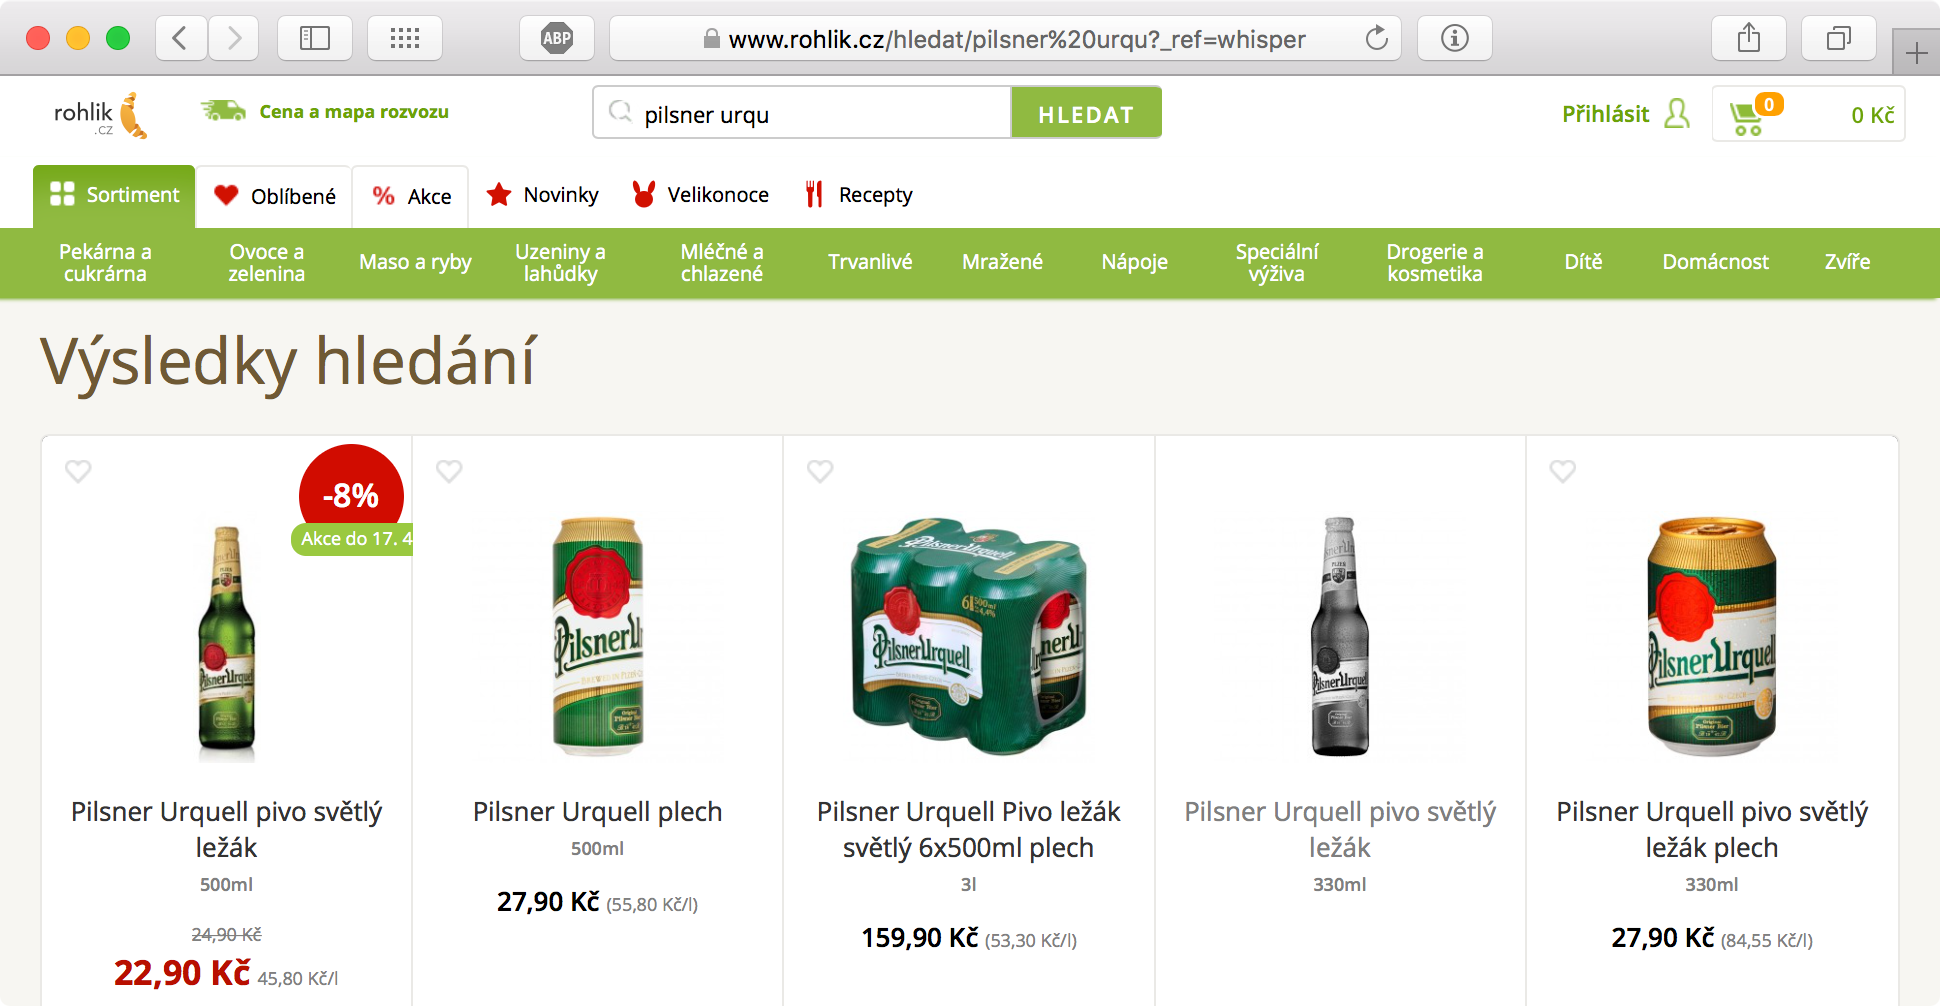
\includegraphics[width=\textwidth]{relevance.png}
\caption[Řazení výsledků]{Řazení výsledků -- upřednostnění akčního zboží na webu rohlik.cz}
\label{relevance}
\end{figure}

Pořadí výsledků nemusí být ovlivňováno jen zájmy provozovatele, mohou jej formovat
sami zákazníci svým chováním. Konkrétně v případě vyhledávání lze pozorovat proklikovost
jednotlivých produktů vzhledem k zadanému dotazu. Pokud se ukáže, že na základě
daného dotazu zákazníci nejčastěji klikají na konkrétní produkt, je možné jej zobrazit 
ve výsledcích vyhledávání pro tento dotaz dříve. 

S tímto přístupem je však možné jít ještě dál a začít vytvářet uživatelské profily zákazníků podle toho, 
o jaké zboží se zajímají, co vyhledávájí, jaké jsou jejich údaje zadané při registraci a objednávce 
(lokalita, pohlaví), nebo v jaké časy nakupují prostřednictvím jakých zařízení. Tato problematika je již
složitější, nicméně v posbíraných datech a vytvořených uživatelských profilech lze hledat další 
souvislosti pomocí statistických metod a strojového učení. Konkrétně lze zákazníka zařadit do určité 
skupiny pomocí shlukové analýzy a podle toho k němu přistupovat (upravit řazení výsledků vyhledávání) 
nebo využít algoritmů doporučovacích systémů.

Samotné řazení všech uložených dokumentů může být výpočetně náročné, v tu chvíli lze řadit
dokumenty ve dvou průchodech. V prvním průchodu jsou nalezeny dokumenty odpovídající zadanému 
dotazu a případně řazeny s pomocí nenáročného výpočtu. Poté lze provést druhé řazení nad výběrem 
prvních dokumentů. Díky tomu, že už probíhá řazení nad malou množinou dat, je možné využít 
výpočetně náročnějších algoritmů.

Výše nastíněné možnosti práce s řazením výsledků jsou však příliš rozsáhlé pro řešení v rámci
této práce. Aktuálně přichází v úvahu "objektivní" řazení dle relevance, to nasadit do provozu.
Poté by bylo vhodné provést pozorování chování zákazníků při vyhledávání a případně využít
některou z~zde uvedených technik pro úpravu pořadí výsledků vyhledávání.

%%%%%%%%%%%%%%%%%%%%%%%%%%%%
\chapter{Návrh řešení vyhledávání}

V této kapitole je popsán návrh aplikace umožňující implementaci plnotextového vyhledávání
do elektronického obchodu, které bude možné provozovat jako službu. Popsán je způsob, 
jakým bude aplikace používána, aktéry, kteří v užívání aplikace vystupují a následně je vytvořen
model, který bude požadavkům nejlépe odpovídat.

\section{Definice případů užití}

Aplikaci používají dva typy uživatelů. \textbf{Správce} (provozovatel elektronického obchodu), který
zajišťuje její konfiguraci (například napojení vstupních dat) a \textbf{zákazník} elektronického
obchodu, který provádí samotné vyhledávání. Z toho vyplývá, že ty části aplikace, které používá 
správce, musí být zabezpečeny, aby k nim neměl přístup nikdo jiný. Navíc musí aplikace umět
pracovat s více správci zároveň, kdy má každý přístup pouze ke svým datům. Pro zákazníka
musí být naopak jeho část aplikace veřejně přístupná, musí být také co nejrychlejší. 
Právě zákazník bude provádět vyhledávání a rychlost, s kterou obdrží výsledky je proto
klíčová.

\begin{figure}[h]
\center
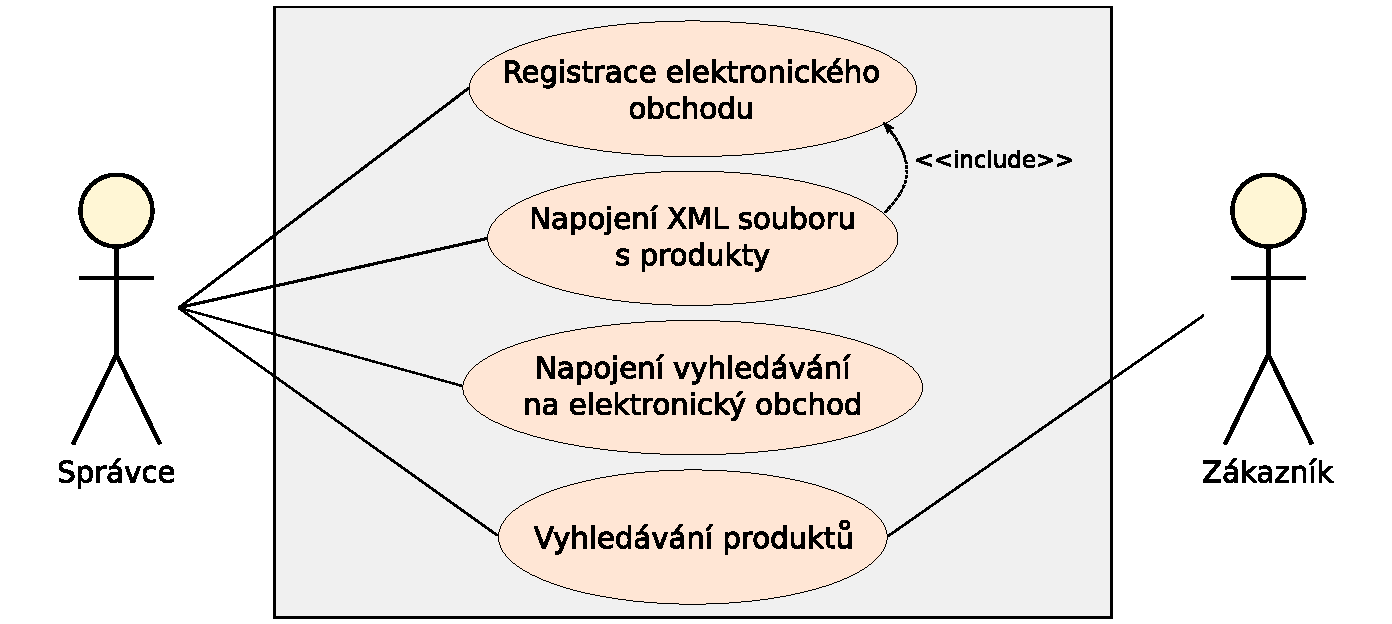
\includegraphics[width=\textwidth]{use-case.pdf}
\caption{Případy užití aplikace}
\label{use-case}
\end{figure}

Na obrázku \ref{use-case} jsou znázorněny základní případy užití z nejméně podrobného pohledu. Jednotlivé 
případy užití jsou popsány podrobně níže.

\subsection{Registrace do aplikace}

Toto je první případ užití a jeho splnění je předpokladem pro další případy užití. Budoucí
správce, který chce aplikaci používat musí mít vytvořen účet, který je přístupný po zadání
jeho přihlašovacích údajů.

\begin{itemize}
\item Správce zobrazí registrační formulář
\item Správce zadá údaje pro svůj ůčet (e-mailová adresa a heslo)
\item Správce zadá adresu souboru XML s produkty a odešle formulář
\item Správce je přihlášen pod novým účtem, je spuštěn import produktů
\end{itemize}

Výsledkem tohoto případu je vytvořený nový účet. Při ukládání systém kontroluje unikátnost
zadaného uživatele a na základě zadané URL produktového XML vytváří novou konfiguraci
daného uživatele a na pozadí spouští import produktů.

\subsection{Napojení XML souboru s produkty}

Tento případ užití lze jednak provést samostatně ve chvíli, kdy je správce přihlášený
do aplikace, je ale také dílčí operací již při registraci.

\begin{itemize}
\item Správce zobrazí formulář pro zadání URL produktového XML
\item Správce zadá adresu souboru XML s produkty a odešle formulář
\item Je spuštěn import produktů na pozadí, je zobrazena informace správci
\end{itemize}

Po provedení tohoto případu užití je aktualizována (nebo vytvořena pokud neexistuje) 
konfigurace daného uživatele. Zároveň je na pozadí spuštěn import produktů, aby byla
zajištěna aktuálnost produktové databáze.

\subsection{Napojení vyhledávání na elektronický obchod}

Ve chvíli, kdy má správce v~aplikaci uložené produkty, může již využít samotné vyhledávání,
které je poskytované jako služba. Toto napojení musí být maximálně intuitivní.

\begin{itemize}
\item Správce se přihlásí do aplikace
\item Správce přejde na stránku zobrazující manuál k implementaci napojení
\item Správce upraví elektronický obchod tak, aby byly požadavky na vyhledávání
směrovány na URL uvedenou v manuálu
\end{itemize}

\subsection{Vyhledávání produktů}

Nejčastějším případem užití je vyhledávání prováděné zákazníkem. To je možné až ve chvíli, 
kdy je implementovaný jak import produktů, tak samotné vyhledávání. 

\begin{itemize}
\item Uživatel v elektronickém obchodu začne psát dotaz do textového pole pro vyhledávání
\item Při každém napsaném nebo smazaném písmenu je odeslán HTTP požadavek na API vyhledávání
\item Pro každý odeslaný požadavek je aktualizován výpis nalezených produktů a tento požadavek
je na serveru zaznamenán
\end{itemize}

Vzhledem k důležitosti tohoto případu je nutné aby bylo vyhledávání rychlé a stabilní.
Každé zpoždění nebo výpadek totiž snižuje důvěru klienta používající vyhledávání.

\section{Návrh architektury aplikace}

S aplikací bude komunikovat správce prostřednictvím grafického webového rozhraní a dále
zákazník, který s aplikací komunikuje prostřednictvím grafického rozhraní elektronického 
obchodu. Ten musí s vyvíjenou aplikací komunikovat prostřednictvím jasně definovaného
a jednoduše implementovatelného API.

Z tohoto důvodu se jeví jako výhodné rozdělit aplikaci na dvě části -- první část (\textbf{backend}) 
bude obstarávat veškerou logiku, perzistenci dat a bude s ní možné komunikovat prostřednictvím API. 
Druhou částí (\textbf{frontend}) by byla samostatná webová aplikace s grafickým rohraním, která 
sama o sobě nepracuje s žádným úložištěm, ale všechny tyto požadavky nechává vyřídit backend \cite{backend}. 
Rozdělení na frontend a backend s sebou nese řadu dalších výhod -- frontend bůže být vyvíjen
v jazyce, který je pro to vhodnější, na obou částech můžou v budoucnu pracovat specializovaní
vývojáři, obě aplikace je možné nezávisle škálovat. Zpřístupněním celého API navíc mohou
vývojáři implementovat celé napojení plně automatizovaně.

Dále je třeba, aby byla architektura navržena tak, aby bylo možné aplikaci snadno škálovat. 
To se týká databáze i samotné aplikace dostupné prostřednictvím API. Databázi je tedy
vhodné volit takovou, která umožní také horizontální škálování \cite{scaling}. Dá se předpokládat, 
že s~rostoucím počtem uživatelů služby bude rovnoměrně růst i potřeba na objem zpracovávaných
dat. S horizontálním škálováním souvisí také možnost vytváření replik dat v úložišti, 
v takovém případě by byl cluster schopný se vyrovnat s případnou ztrátou některých dat.
S možností snadného vertikálního škálování aplikace je třeba počítat při jejím nasazování.
Prostředí, do kterého bude aplikace nasazována by mělo být schopné aplikaci škálovat
obdobně jako databáze. Díky tomu, že veškerá data jsou persistována v databázi, je možné
průběžně zapínat a vypínat jednotlivé instance aplikace bez obavy o ztrátu dat.\\

Na obrázku \ref{architektura} je znázorněn vztah mezi jednotlivými komponentami aplikace včetně
napojovaného elektronického obchodu. Dále jsou zde zobrazeni oba aktéři -- zákazník i správce.

\begin{figure}[h]
\center
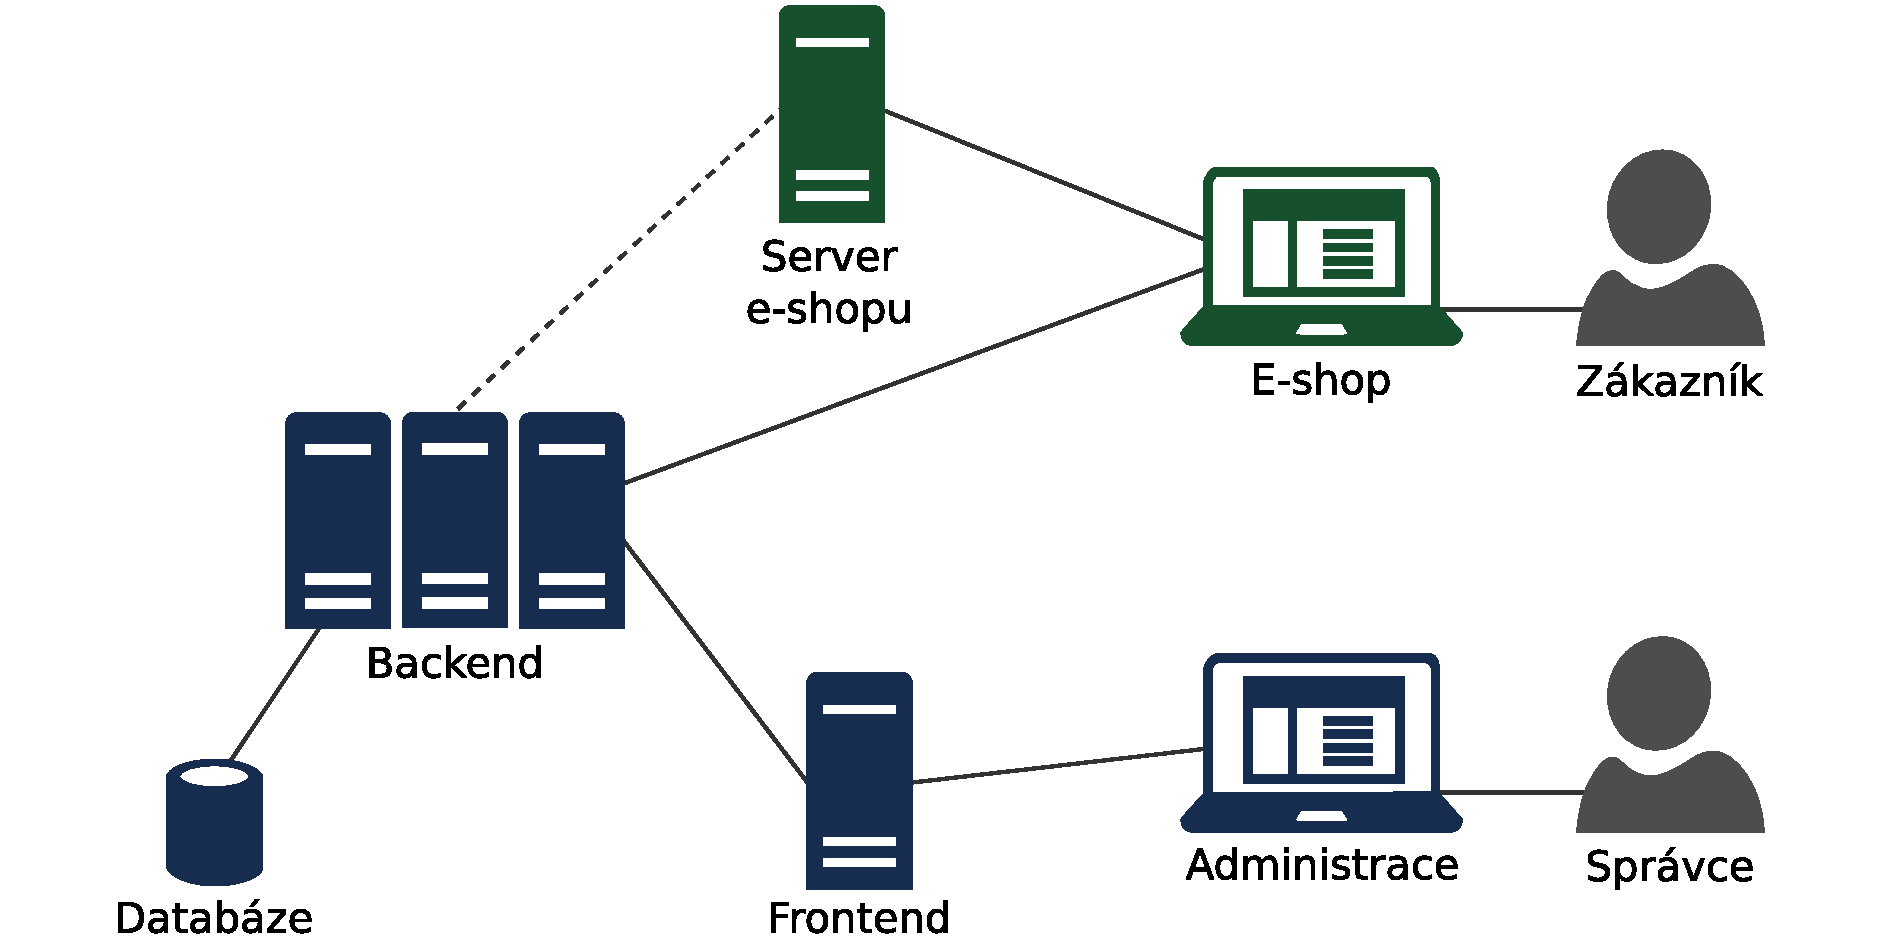
\includegraphics[width=\textwidth]{architektura.pdf}
\caption[Architektura aplikace]{Architektura aplikace -- propojení dílčích komponent}
\label{architektura}
\end{figure}

Ze schématu je zřejmé, že zákazník si zobrazuje elektronický obchod, který je zobrazen
na základě dat z serveru obchodu. Data pro vyhledávání jsou načtena prostředníctvím API 
aplikce, přičemž požadavek může být odeslán přímo z webového prohlížeče zákazníka 
(asynchronní HTTP požadavek) nebo prostřednictvím serveru obchodu (pokud probíhá vykreslení 
HTML stránky na serveru). Z druhé strany s aplikací operuje správce, který ji ovládá skrze
administraci, která disponuje grafickým webovým rozhraním. Ta však veškeré požadavky
směřuje na backend. Konečně backend používá pro persistenci dat (produktů i konfigurací)
databázi, ostatním službám je pak dostupný skrze API.

\section{Datový model}

V této části jsou definovány entity, které v aplikaci vystupují, jejich atributy a vztahy mezi 
nimi. V systému primárně vystupuje \textbf{uživatel} (správce), který se do aplikace registroval 
a vytváří konfiguraci pro import produktů. Pro každou tuto konfiguraci jsou do systému
importovány produkty, jejichž struktura byla rozebrána v analýze dat, v kterých bude 
vyhledáváno. 

U uživatele je zvolen jako jeho přirozený jednoznačný identifikátor jeho e-mailová
adresa, kterou zadává při registraci. Dále je třeba uložit jeho heslo (respektive
jeho hash) pro umožnění přihlášení. Posledním atributem uživatele je náhodně vygenerovaný
token, který bude využit při přístupu k API klientem. Je totiž třeba zajistit, 
aby nebylo možné triviálním způsobem procházet produkty dalších uživatelů 
\cite[strana~16]{api}.

Uživatel si dále vytváří konfiguraci, ve které je uložena adresa s XML souborem 
obsahujícím produkty, informace o jeho formátu (v případě že bude podporováno více
formátů, je to vhodné pro detekci formátu a použití vhodného parseru). Tato 
\textbf{konfigurace} náleží právě jednomu uživateli, v jiných případech nemá 
její existence význam.

Další entitou, s kterou je třeba pracovat je \textbf{produkt} -- právě ten bude vyhledáván.
Jeho atributy v nejjednodušší podobě jsou jeho jednoznačný identifikátor nebo kód
(v rámci daného obchodu), název, popis, URL, adresa obrázku a cena. Produkt je možné
rozšířit o další atributy, nicméně toto jsou atributy, které by měly být u každého
produktu známy.

\begin{figure}[h]
\center
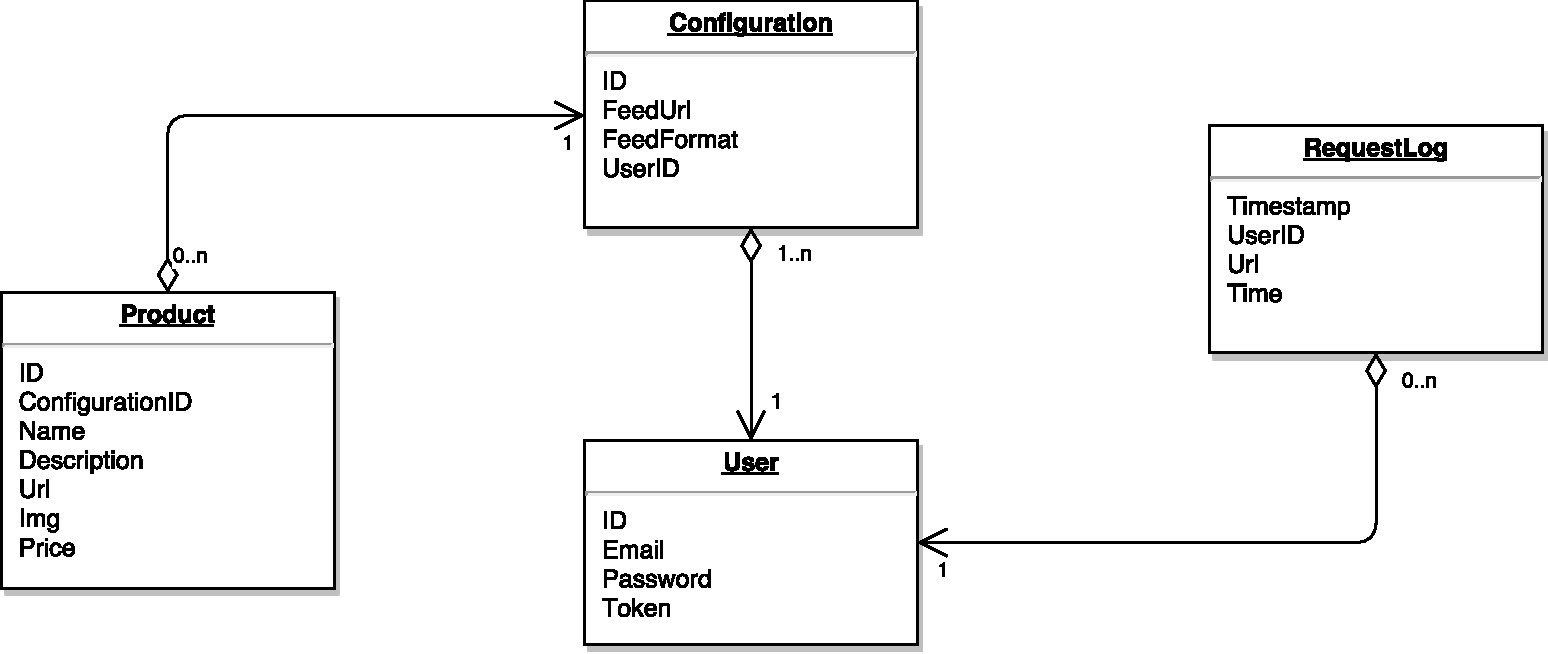
\includegraphics[width=\textwidth]{era-diagram.pdf}
\caption[Datový model aplikace]{Datový model aplikace (ERA diagram)}
\label{datovy-model}
\end{figure}

Poslední entitou znázorněnou v diagramu \ref{datovy-model} je zalogovaný požadavek. 
Vzhledem k tomu, že chceme mít jednak kontrolu nad rychlostí vyhledávání, tak je dobré mít
přehled o využití aplikace ať už jako celku, tak vzhledem k jejímu využití jednotlivými
obchody. Každý takový záznam musí obsahovat datum a čas, kdy byl zaznamenán, 
URL, na kterou byl požadavek odeslán a čas, který trvalo jeho vyřízení.

\section{Návrh API}

Klíčový je návrh API, jehož prostřednictvím je dostupná veškerá logika aplikace. 
Při jeho návrhu jsem se rozhodl využít přístupu design-first \cite{apiary-design}, 
kdy je nejprve navrženo samotné API (vytvořena jeho dokumentace) a až poté je přistoupeno 
k~samotné implementaci. Pro jeho návrh je využíván nástroj Apiary \cite{apiary}, který 
umožňuje pracovat s~API podle tohoto přístupu.

Před konkrétním návrhem je třeba rozmyslet protokol a další principy, kterých API využívá.
Přestože by se mohlo zdát, že to je až záležitost samotné implementace, tento krok zásadně
ovlivňuje již způsob návrhu API. Dále je to důležité k použití přístupu design-first.

Pro naplnění požadavků vycházejících z informací o problematice elektronického obchodování
je třeba volit takový protokol, který je běžně dostupný napříč všemi běžnými webovými
prohlížeči a je možné jej využít v používaných webových technologiích. Takovým protokolem
je HTTP (případně novější verze HTTP/2). V~nejnovějších prohlížečích by sice bylo možné
používat pokročilejší protokoly (například WebSockets \cite{websockets}), aktuálním cílem
je však maximální možná kompatibilita a snadnost implementace. Samotná komunikace probíhá
dle principu REST, data jsou zasílána ve formátu JSON, což jsou nejpřímočařejší způsoby
návrhu a implementace \cite{api}. Bylo by možné využít jiných mechanismů (XML-RPC nebo SOAP), 
nicméně pro tento konkrétní případ jsou méně vhodné vzhledem k jejich snadnosti implementace, 
pochopitelnosti a rychlosti \cite[strana~31]{api}.

\subsection{Datové struktury}

Nejprve je třeba identifikovat zdroje (resources), což jsou datové struktury, které
budou prostřednictvím API předávány. Dále je třeba definovat operace, které lze nad 
jednotlivými zdroji provádět (čtení, vytváření, mazání, aktualizace) a nakonec také 
vhodně navrhnout koncové body (endpoints) \cite[strana~12]{api}, pod kterými bude každá 
operace dostupná.

Základní zdroje, s kterými API operuje jsou \textbf{produkt} a \textbf{konfigurace uživatele}. 
Tyto struktury nesou důležitou informační hodnotu, první veškeré informace o produktu, 
které může být třeba v elektronickém obchodu zobrazit, druhá pak informace o nastavení 
daného uživatele. Tyto struktury lze popsat pomocí syntaxe API Blueprint \cite[strana~131]{api}
následovně:

\begin{code}
\captionsetup{singlelinecheck=false,justification=raggedright}
\captionof{listing}{Dokumentace API -- struktura produktu}
\label{code:api-product}
\begin{minted}{md}
# Data Structures

## Product (object)
- id: `1mWa9` (string, required) - ID of product
- userId: `01dsdmmwv2dwkdlam8di8` (string, required) - User ID
- name: `Postel bílá` (string, required) - Name of product
- description: `Postel vyrobena z masivu...` (string, required) - Product description
- url: `http://shop.tld/1mWa9` (string, required) - detail URL
- img: `http://shop.tld/1mWa9.jpg` (string, required) - image URL
- price: `1` (number, required) - Current price of product incl. VAT
- updated: `2016-12-04T23:22:16+01:00` (string, optional) - Timestamp of last update
\end{minted}
\end{code}

\begin{code}
\captionsetup{singlelinecheck=false,justification=raggedright}
\captionof{listing}{Dokumentace API -- struktura nastavení uživatele}
\label{code:api-user}
\begin{minted}{md}
## UserConfig (object)
- id: `01dsdmmwv2dwkdlam8di8` (string, required) - User ID
- token: `7Tnl6xPQhVPiv80ryboo4iTckqXVuG4xjWFXTC1mzU3EaGY5` (string, required) - security token for API access
- email: `user@email.com` (string, required) - e-mail address
- password: `p4ssw0rd` (string, optional) - new password
- feedUrl: `http://shop.tld/feed.xml` (string, required) - XML feed
- feedFormat: `heureka` (enum[string], required)
    - `heureka`
\end{minted}
\end{code}

Zde struktura \Verb|Product| bude používána pouze pro čtení, produkty jsou vytvářeny
na základě importovaného XML souboru. Konfigurace uživatele je používána jak při
registraci (vytvoření nové konfigurace), tak při aktualizaci této konfigurace (čtení
i změna).

Dalšími pomocnými strukturami jsou data pro provedení \textbf{přihlášení} správce 
do administrace. Ten při přihlášení zadává přihlašovací jméno a heslo, jako odpověď 
obdrží své ID a dále token, identifikující jeho sezení a použitelný pro vykonání 
dalších požadavků.

\begin{code}
\captionsetup{singlelinecheck=false,justification=raggedright}
\captionof{listing}{Dokumentace API -- struktura požadavků a odpovědí serveru}
\label{code:api-request}
\begin{minted}{md}
## LoginRequest (object)
- email: `user@email.com` (string, required) - e-mail address
- password: `p4ssw0rd` (string, required) - password

## LoginResponse (object)
- userId: `01dsdmmwv2dwkdlam8di8` (string, required) - id of user
- token: `JT0n0rws8rRMx8P205hmc68c9yptDW91PkuLNcHe2J2NxQdyO` (string, required) - auth token
\end{minted}
\end{code}

Poslední struktury, které API používají, definují formát odpovědi pro operace, které
neočekávají žádná data, pouze je modifikují (mutace). Po provedení takových operací
API informuje o úspěšnosti jejich provedení odpovídajícím stavovým kódem. V případě 
neúspěchu přidává srozumitelnou hlášku včetně detailního popisu o důvodu neúspěchu, 
což usnadňuje práci vývojářum napojovaných aplikací a odstraňování chyb \cite[strana~42]{api}.

%## Ok (object)
%- status: `200` (number, required) - HTTP status code
%- message: `User created` (string, optional) - Result message

\begin{code}
\captionsetup{singlelinecheck=false,justification=raggedright}
\captionof{listing}{Dokumentace API -- struktura odpovědi v případě chyby}
\label{code:api-error}
\begin{minted}{md}
## Error (object)
- status: `400` (number, required) - HTTP status code
- message: `Unable to create user` (string, required)
- description: `Email already exists` (string, optional)
\end{minted}
\end{code}

\subsection{Koncové body}

Pro každou operaci je definován koncový bod (endpoint) a metoda, pomocí které je operace
dostupná, přičemž koncový bod je URL, pod kterou je dostupný \cite{api}. Ta je uváděna relativně
vzhledem k doméně, pod kterou je aplikace provozována. Dále všechny mají adresy
prefix \verb|/api/v1|, který usnadní možné budoucí aktualizace, které nejsou zpětně kompatibilní.

Koncové body jsou pojmenovány podle zdrojů, s kterými pracují, aby bylo jejich používání 
intuitivní. Prvními jsou body pro provedení přihlášení a odhlášení, které operují
s zdroji \textbf{LoginRequest} a \textbf{LoginResponse}, respektive \textbf{Ok} a \textbf{Error}.

\begin{itemize}
\item \verb|POST /api/v1/sign/in| -- přihlášení do administrace
\item \verb|POST /api/v1/sign/out/{token}| -- odhlášení z administrace
\end{itemize}

Další množina bodů provádí operace se zdrojem \textbf{UserConfig}. Slouží pro registraci
nového uživatele, aktualizaci údajů stávajícího uživatele, zobrazení registračních údajů
a případnou deaktivaci účtu stávajícího uživatele.

\begin{itemize}
\item \verb|GET /api/v1/user/{token}| -- získání konfigurace uživatele
\item \verb|PUT /api/v1/user/{token}| -- vytvoření nebo aktualizace konfigurace
\item \verb|DELETE /api/v1/user/{token}| -- deaktivace uživatele
\end{itemize}

Posledním koncovým bodem je vyhledávání produktů. Tento bod je jediný veřejný a použitý
v elektronickém obchodě. Tento bod přejímá dva paramtery, kterými jsou ID uživatele
(obchodu) a hledaný výraz. Data jsou získávána jako pole objektů \textbf{Product}, 
které je ještě zanořeno v dalším poli, kde je dostupné pod klíčem \verb|products|.
To usnadní budoucí možné rozšiřování o další data (výsledky agregačních dotazů nebo 
například stav stránkování) s zachováním zpětné kompatibility.

\begin{itemize}
\item \verb|GET /api/v1/search/{userId}/{query}| -- vyhledání produktů dle \verb|query|
\end{itemize}

Tento koncový bod musí být v administraci aplikace zadokumentován a uveden s názornými 
příklady, jak jej napojit do elektronického obchodu na základě konkrétní použité technologie.

Celé API je dokumentováno v formátu API Blueprint a je distribuováno společně s zdrojovými
kódy aplikace, které jsou přílohou této práce. Současně je vytvořen projekt v nástroji 
Apiary, ve kterém je dokumentace uložena a veřejně přístupná pod URL 
\url{http://docs.apisearch.apiary.io}. Ta obsahuje i vzorová data, 
je tedy možné využít serverů proxy, které umožňují přistupovat k API, které vrací ukázková 
data. Je tedy možné začít nezávisle na sobě navrhovat a vyvíjet stranu, která API poskytuje
(backend) i konzumuje (frontend). Vytvořený soubor ve formátu API Blueprint budiž smlouvou, 
která mezi těmito aplikacemi vznikla.

%\section{Indexace dokumentů}
%... TODO ... teoreticky to rozebrat


%%%%%%%%%%%%%%%%%%%%%%%%%%%%
\chapter{Implementace vyhledávání jako služby}

V této kapitole je popisována implementace na základě předchozího návrhu. Okomentováno je
zde vše spojené s implementací, od výběru vhodných nástrojů přes samotnou implementaci
a konfiguraci zvolených nástrojů až po nasazení do produkčního prostředí.
text může sloužit jako návod pro implementaci vyhledávání poskytovatelného jako
služba, kompletní zdrojové kódy jsou pak dostupné v příloze.

\section{Výběr nástroje pro vyhledáváni}

Nejprve je třeba zvolit nástroj, který bude použit pro samotné vyhledávání. To podporují 
jak běžně používané relační databáze, tak specializované nástroje. U relačních databází
jde spíše o rozšíření jejich funkčnosti a naopak -- specializované nástroje lze použít
jako databáze. Zde je třeba rozhodnout, který z těchto nástrojů bude nejlépe vyhovovat
požadavkům na vyhledávání.

\subsection{PostgreSQL}

PostgreSQL (nebo také Postgres) je jedna z open-source relačních databází, která podporuje
mnoho funkcí, které jsou dobře použitelné pro implementaci kvalitního plnotextového 
vyhledávání. Pro vyhledávání textu, který nepodléhá tvarosloví je možné využít operátorů
\verb|~|, \verb|~*|, \verb|LIKE| a \verb|ILIKE|. Dále tato databáze umožňuje zpracování
textu již při ukládání (indexaci) \cite{postgres-search}. Do databáze lze uložit slovníky, 
které lze následně využít pro:

\begin{itemize}
\item Definici stop slov
\item Mapování slov na jiná -- synonyma pomocí \verb|Ispell| a fráze pomocí tezauru
\item Transformaci slov do jejich základní formy pomocí slovníku \verb|Ispell| a pomocí \
pravidel stemmeru \verb|Snowball|
\end{itemize}

Dále disponuje funkcemi pro implementaci fuzzy vyhledávání, konkrétně \verb|levenshtein()|
a \verb|metaphone()|. Mezi nevýhody patří obtížnější instalace a konfigurace. Zejména, 
pokud bude třeba databázi škálovat.

\subsection{Elasticsearch}

Elasticsearch vznikl primárně jako nástroj pro textové vyhledávání, podporuje tak
mnoho funkcí, které jsou pro textové vyhledávání použitelné. Interně používá
Apache Lucene, rozšiřuje jej však o řadu funkčnosti a usnadňuje práci s ním
používáním vlastního API. Dále je od počátku navržen jako distribuované úložiště, 
škálování tedy spočívá pouze v přidávání uzlů. Elasticsearch poté sám vytváří
repliky dat a distribuje je napříč clusterem \cite{elastic}. 

Umožňuje import slovníků, nastavení řady filtrů pro indexaci (synonyma, n-gramy, stematizaci, 
lematizaci a celou řadu dalších filtrů a analyzátorů \cite{es-analysis}). Zároveň umožňuje
precizně nastavit výpočet relevance, nad daty lze vypočítávat agregace, vše je navíc
velmi rychlé a rychlost se zásadně nemění s přibývajicími daty. Elasticsearch je výrazně 
rychlejší ve srovnání s PostgreSQL -- \cite{es-postgres} a \cite{es-postgres-2}.

\subsection{Apache Solr}

Dalším nástrojem, který přichází v úvahu je Apache Solr \cite{solr}. Shodně jako Elasticsearch 
využívá interně Apache Lucene. Co se funkčnosti týče, je tedy téměř srovnatelný s použitím
Elasticsearch. Ten jej však převyšuje intuitivností instalace, snadnější možností použití 
analytických dotazů a výkonností a stabilitou vzhledem ke škálování \cite{es-solr}. Přestože 
aktuálně nejsou zmíněné výhody tolik důležité, vzhledem k očekávanému rozšiřování je vhodné 
je vzít v potaz a dále tak uvažuji pouze nad Elasticsearch. Do závěrečného porovnání jej
nezahrnuji, protože kromě výše uvedených nuancí by bylo hodnocení obdobné.

\subsection{Sphinx}

Posledním nástrojem, který přichází v potaz je Sphinx Search \cite{sphinx}. Ten se zaměřuje 
především na rychlost, je napsán v C++, je také relativně nenáročný na paměť. 
Pro potřeby vyhledávání má dostatek funkcí, neumí ale nic jiného, zaměřuje se
pouze na textové vyhledávání.

Na rozdíl od výše uvedených nástroj Sphinx není úložiště. Je nutné jej provozovat
jako nadstavbu nad stávající databází (například MySQL nebo Oracle). Sphinx umí pouze 
indexovat dokumenty a následně v nich vyhledávat, jejich načtení již však musí být provedeno 
odjinud. Provoz s další databází by tedy v tomto případě znamenal zbytečné zesložitění architektury. 

Jeho použití by ale bylo daleko vhodnější, pokud by již byla jiná databáze využívána a pouze 
ji bylo třeba rozšířit o pokročilé textové vyhledávání. V takovém případě není třeba
přecházet na jiné úložiště, pouze je rozšířena stávající funkčnost o plnohodnotné
textové vyhledávání.

\subsection{Porovnání nástrojů pro vyhledávání}

V následující tabulce je zobrazeno přehledné porovnání dle parametrů které jsou klíčové pro 
tento projekt. 

\begin{table}[h!]
\captionsetup{singlelinecheck=false,justification=raggedright}
\caption{Porovnání nástrojů pro vyhledávání}
\label{search-comp}
\centering
\begin{tabular}{ll}  
\toprule
&\multicolumn{1}{c}{\textbf{Obecný popis}} \\
\cmidrule(r){2-2}
PostgreSQL    & Relační databáze umožňující textové vyhledávání \\
Elasticsearch & Textové vyhledávání a škálovatelné úložiště \\
Sphinx        & Textový vyhledávač \\
\midrule
\midrule
&\multicolumn{1}{c}{\textbf{Snadnost instalace a konfigurace}} \\
\cmidrule(r){2-2}
PostgreSQL    & Snadná základní instalace, obtížnější pokročilá konfigurace \\
Elasticsearch & Intuitivní instalace, zabezpečení, monitoring nutné řešit pluginy \\
Sphinx        & Snadná instalace \\
\midrule
\midrule
&\multicolumn{1}{c}{\textbf{Škálování}} \\
\cmidrule(r){2-2}
PostgreSQL    & Obtížné na konfiguraci \\
Elasticsearch & Triviální, horizontální škálování je automaticky předpokládáno \\
Sphinx        & Závislé na použité databázi \\
\midrule
\midrule
&\multicolumn{1}{c}{\textbf{Výkonnost}} \\
\cmidrule(r){2-2}
PostgreSQL    & Ryhlé pro jednoduché dotazy, s složitostí výkonnost klesá \\
Elasticsearch & Rychlé -- automatická paralelizace, cachování \\
Sphinx        & Velmi rychlé a nenáročné na paměť\\
\midrule
\midrule
&\multicolumn{1}{c}{\textbf{Textové vyhledávání}} \\
\cmidrule(r){2-2}
PostgreSQL    & Podporuje většinu běžných funkcí \\
Elasticsearch & Propracované \\
Sphinx        & Propracované \\
\midrule
\midrule
&\multicolumn{1}{c}{\textbf{Podpora (dokumentace, literatura)}} \\
\cmidrule(r){2-2}
PostgreSQL    & Dostatečně dokumentováno, množství dostupné literatury \\
Elasticsearch & Podrobná dokumentace, profesionální podpora za poplatek \\
Sphinx        & Dostatečně dokumentováno \\
\bottomrule
\end{tabular}
\end{table}

Na základě porovnání vychází vzhledem k požadavkům nejlépe použití Elasticsearch, 
přestože využití ostatních zmíněných nástrojů by bylo také možné. Elasticsearch
je ale vhodný zejména díky výkonnosti, která se zásadně nemění díky možnostem škálování, 
množstvím podporovaných filtrů a analyzátorů a také množstvím dalších funkcí, 
které by mohly být využity v budoucnu, bez nutnosti přechodu na jinou technologii.

\section{Nastavení a nasazení Elasticsearch}

Aplikace využívá Elasticsearch verze 5.1.2. Jedná se o aktuální verzi, která však
může být v době čtení této práce zastaralá, protože vydávání nových verzí probíhá
velmi často. Principy zde popsané se však nemění a s největší pravděpodobností 
budou ukázky fungovat i v~novějších verzích Elasticsearch.

V rámci Elasticsearch se pracuje s pojmy, které je pro orientaci třeba vysvětlit:

\begin{itemize}
\item \textbf{Cluster} je několik (alespoň jeden) serverů komunikujících spolu
\item \textbf{Node} je jedna spuštěná instance Elasticsearch, odpovídá jednomu serveru
\item \textbf{Index} je skupina dokumentů, které mají společnou charakteristiku
\item \textbf{Type} je skupina souvisejících dokumentů v rámci indexu
\item \textbf{Document} je jedna zaindexovaná položka
\item \textbf{Field} je atribut dokumentu (například název produktu, kde produkt je dokument a název je atribut)
\item \textbf{Shard} je část indexu Elasticsearch (index Apache Lucene), umožňuje data fyzicky
v indexu rozdělit a distribuovat je napříč clusterem
\item \textbf{Replica} je kopie shardu, záloha umístěná na jiném node
\end{itemize}

S Elasticsearch se komunikuje přes REST API, kdy je možné zasílat dokumenty ve formátu JSON.
To umožňuje snadnou implementaci klientských knihoven nebo komunikaci s serverem
z příkazové řádky nebo pomocí univerzálních nástrojů pro práci s API.

\subsection{Vytvoření Docker obrazu}

Pro lokální vývoj i produkční nasazení
je využíván Docker, což je nástroj umožňující běh aplikací v izolovaném prostředí
\cite{docker}. Umožnuje vytvoření identického prostředí, ať už je aplikace spouštěna 
lokálně, při testech nebo v produkčním prostředí. Základním artefaktem je obraz (Docker
image), který po spuštění vytvoří kontejner. Vztah obraz -- kontejner lze chápat jako 
analogii k~vztahu program -- proces. Pro vytvoření Docker obrazu slouží soubor \verb|Dockerfile|,
což je vpodstatě sada kroků (příkazů) vedoucí k požadované podobě obrazu.

\begin{code}
\captionsetup{singlelinecheck=false,justification=raggedright}
\captionof{listing}{Dockerfile pro Elasticsearch}
\label{code:dockerfile}
\begin{minted}{docker}
# Základní obraz - oficiální Elasticsearch v Alpine Linux
FROM elasticsearch:5.1.2-alpine

# Instalace pluginu ICU
RUN bin/elasticsearch-plugin install analysis-icu

# Kopírování složky obsahující konfiguraci a slovníky
ADD config config/
\end{minted}
\end{code}

V souboru \verb|Dockerfile| \ref{code:dockerfile} je definováno z~jakého
základního obrazu vychází a dále posloupnost kroků vedoucí k vytvoření požadovaného obrazu.
Zde je zvolena oficiální verze Elasticsearch instalovaná v Apline Linux, což je minimalistická 
linuxová distribuce zaměřená na bezpečnost \cite{alpine}. Vychází z knihoven \verb|musl libc| 
a programu \verb|busybox| a přichází s principem, že Linuxová distribuce v základu
nedisponuje téměř žádnými nástroji a je na uživateli, co si doinstaluje. To má příznivý
vliv na velikost a rychlost. Taková distribuce je i bezpečnější -- je minimalizováno 
množství míst, která mohou vést k~zranitelnosti systému. Tento přístup je pro vytváření
kontejnerů žádoucí a tak je distribuce Apline Linux využívána stále častěji
i v oficiálních obrazech \cite{alpine-lean}.

Pro potřebu této práce je doinstalován plugin ICU, který je nutný pro korektní práci 
s~českými znaky. Dále je do obrazu nakopírována složka \verb|config| obsahující konfiguraci
Elasticsearch v souboru \verb|elasticsearch.yml| (výchozí název clusteru a porty, přes které 
je Elasticsearch dostupný) a slovníky Hunspell \cite{hunspell}. To jsou slovníky obsahující 
českou slovní zásobu a veškeré informace potřebné pro morfologickou analýzu. Běžně jsou používány 
ve~volně dostupných aplikacích jako jsou LibreOffice \cite{hunspell-download} nebo Mozilla Firefox. 
Slovník je tvořen dvěma soubory, v~případě češtiny jsou to soubory \verb|cz_CZ.dic| a \verb|cz_CZ.aff|. 
První soubor obsahuje slovní zásobu, příčemž u každého slova jsou uvedeny příznaky, 
které definují, jakým slovem je slovo ohýbáno. V druhém slovu je popsána morfologie českého
jazyka -- pro každý příznak je definováno, jakým způsobem jsou odvozovány další tvary
slova \cite{hunspell-man}.

Tento kód je sdílen prostřednictvím služby GitHub, která je napojena na Docker Hub. 
Obdobným způsobem, jako je sdílen kód prostřednictvím verzovacích nástrojů (VCS --
například GIT nebo SVN) lze i sdílet obrazy Docker. Jako vzdálené úložiště (obdoba 
\verb|origin| pro GIT) je použito tak zvaný registr (Registry), kterým je standardně
Docker Hub. Provázání mezi GitHub a Docker Hub je na té úrovní, že při aktualizaci 
kódu v~repozitáři (provedení příkazu \verb|git push|) je automaticky spuštěno sestavení 
nového obrazu v službě Docker Hub (příkaz \verb|docker build| a následně \verb|docker push|).
Po sestavení obrazu je nahrán do registru a od té doby je připraven ke stažení a spuštění.
Sestavený obraz je možné stáhnout prostřednictvím příkazu \verb|docker pull apisearch/elasticsearch|
a lze jej využít jak pro lokální vývoj, tak pro produkční nasazení.

\subsection{Nastavení indexace v Elasticsearch}

Dále je třeba Elasticsearch nastavit pro správnou indexaci dokumentů. Jednotivá pole indexovaného
dokumentu jsou rozdělena na slova pomocí tokenizéru, vzniklé tokeny jsou dále zpracovány filtry, 
které provádí dílčí transformace. Ty lze řetězit a vytvořit tak analyzér, který popisuje
celý proces.

%\begin{figure}[h]
%\center
%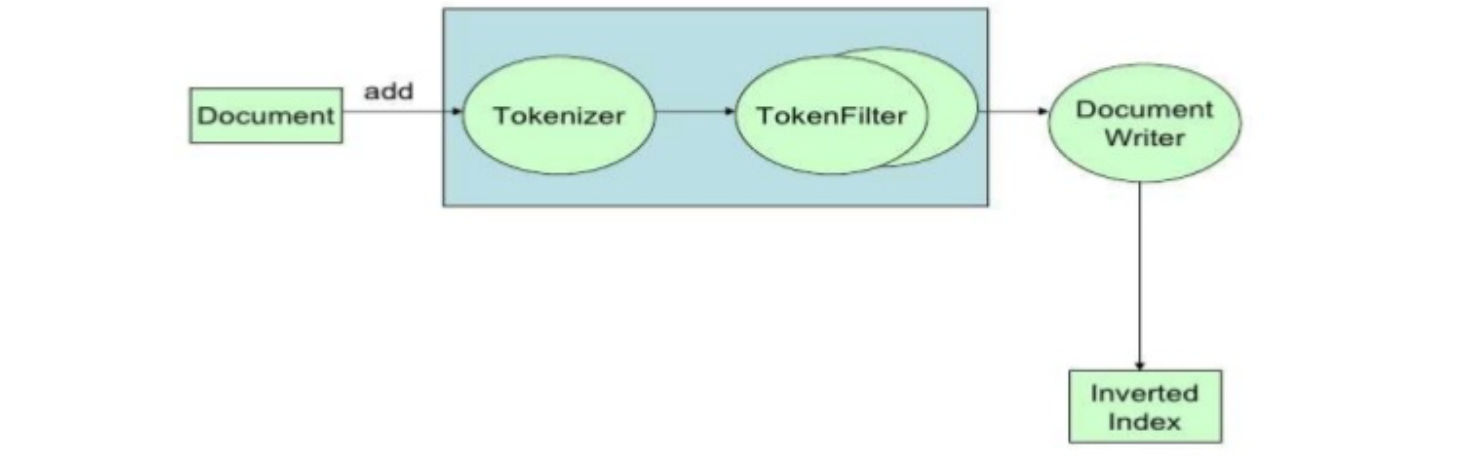
\includegraphics[width=\textwidth]{es-indexace.png}
%\caption{Indexace dokumentů v Elasticsearch}
%\label{es-indexace}
%\end{figure}

První používaný filtr je typu \verb|length|, který má na starosti odstranění slov skládajících
se z~jediného písmena. Následně je definován filtr pro odstranění stop slov \verb|stop|.
Ten využívá výchozí databázi stop slov rozšířitelnou o libovolná další slova. Další filtr
je typu \verb|unique| a stará se o odstranění duplicitních slov. Nemá totiž smysl mít v indexu
uloženo slovo vícekrát, již nepřináší další informační hodnotu. Tyto filtry rozhodují, 
zda bude dané slovo uloženo do invertovaného indexu. Uložit je lze do nastavení indexu
následovně voláním HTTP požadavku metodou \verb|PUT| na koncový bod \verb|/products/_settings| 
(předpokládán je název indexu \verb|products|) s následujícími daty:

\begin{code}
\captionsetup{singlelinecheck=false,justification=raggedright}
\captionof{listing}{Nastavení filtrů pro indexaci v Elasticsearch (1/2)}
\label{code:es-filters-1}
\begin{minted}{json}
{ "settings": {
    "analysis": {
      "filter": {
        "min_length": {
          "type": "length", "min": 2
        },
        "stopwords": {
          "type": "stop", "ignore_case": true, 
          "stopwords": ["že", "právě", "_czech_"]
        },
        "unique": {
          "type": "unique", "only_on_same_position": "false"
        },
        "..."
\end{minted}
\end{code}

Další filtry mají na starost transformaci slov -- převedení do základního tvaru, 
úpravu velikosti písmen nebo generování n-gramů. Velká písmena na malá převádí filtr 
\verb|lowercase|. Díky tomu lze vyhledávat nezávisle na velikosti písmen, která uživatel zadává. 
Filtr, který převádí slova na jejich základní tvar se nazává \verb|hunspell|. Ten využívá
k převodu slovník huspell, který je již nainstalován do používané distribuce Elasticsearch.
Zvláštním filtrem je \verb|shingle|, který v podstatě vytváří n-gramy, činí tak ale na úrovni 
celých slov. Nastavení těchto filtrů lze provést následovně:

\begin{code}
\captionsetup{singlelinecheck=false,justification=raggedright}
\captionof{listing}{Nastavení filtrů pro indexaci v Elasticsearch (2/2)}
\label{code:es-filters-2}
\begin{minted}{json}
{       "...",
        "lowercase": {
          "type": "lowercase", "min": 4
        },
        "shingle": {
          "type": "shingle", "max_shingle_size": 3
        },
        "hunspell": {
          "type": "hunspell", "locale": "cs_CZ", "dedup": true
        },
        "synonym": {
           "type": "synonym", "synonyms_path": "th_cs_CZ.dic"
        }
}
\end{minted}
\end{code}

Posledním filtrem, který by bylo možné použít je zpracovávající synonyma, který se jmenuje 
\verb|synonym|. Tomuto filtru lze předat pod parametrem \verb|synonyms_path| cestu
k~souboru, v~němž jsou synonyma uložena. Ta mohou být ve více formátech - podporován
je formát Solr, kde jsou všechna související synonyma na jednom řádku oddělena čárkou,
nebo ve formátu WordNet, což musí být definováno parametrem \verb|format|.
Je otázkou, jak synonyma získat, protože Elasticsearch sám o sobě žádným jejich
slovníkem nedisponuje. Jistou možností je použít již existující slovník WordNet, 
ten je však nesmírně drahý \cite{wordnet}. Nabízí se tedy možnost opět využít slovníků
Hunspell, které je možné stáhnout z webu OpenOffice \cite{hunspell-download}.

Slovník synonym je možné dále rozšiřovat na základě praktické zkušenosti a poznatků
z proběhlých vyhledávání -- stažený slovník jistě nebude obsahovat všechna myslitelná
synonyma. Pro tento účel by bylo možné definovat další filtr, který však bude využívat
vlastní soubor synonym. Problém však je, že při každé změně bude třeba přeindexovat
všechna data, což s sebou přináší zvýšenou zátěž po dobu indexace.

Nyní zbývá připravit analyzéry, které lze chápat jako řadu filtrů, které jsou zřetězeny, 
sekvenčně zpracovávají obdržený text, přičemž vstupem filtru je výstup filtru předchozího. Využít 
lze filtrů standardních nebo vlastních (definovaných výše). Dále je možné jedno pole nechat indexovat
prostřednictvím více analyzérů a v těchto polích vyhledávat s rozdílnou váhou. 

Analyzér používaný pro vyhledávání v názvu produktu se skládá z~filtru \verb|icu_folding| 
(který byl instalován při vytváření Docker obrazu jako plugin) a z~filtrů definovaných výše.
Dále je třeba v rámci nastavení analyzéru zvolit tokenizér, což je nástroj, který dělí textový
řetězec na slova. Nastavení analyzéru vypadá následovně:

\begin{code}
\captionsetup{singlelinecheck=false,justification=raggedright}
\captionof{listing}{Nastavení analyzátorů v Elasticsearch}
\label{code:es-analyzers}
\begin{minted}{json}
{ "settings": {
    "analysis": {
      "filter": { "..." }
      "analyzer": {
        "icu": {
          "filter": [
            "icu_folding",
            "min_length",
            "hunspell",
            "synonym",
            "stopwords",
            "unique"
          ],
          "tokenizer": "standard"
        }
      }
} } }
\end{minted}
\end{code}

Zbývá doplnit nastavení indexu, které nesouvisí přímo s~indexací, ale s~provozem Elasticsearch.
Jednou z těchto konfigurací je nastavení počtu fragmentů (shards) a replik (replicas).
Pro lokální vývoj nemá smysl jiné nastavení než počet fragmentů roven jedné a počet
replik roven nule. Pokud není spuštěn Elasticsearch v režimu clusteru (neexistuje více uzlů), 
není jednoduše kam repliky ukládat. Stejně tak nemá smysl vytvářet více fragmentů, které
znamenají pouze vyšší režii souborového systému. V produkčním prostředí je však situace jiná --
vše se však odvíjí od množství dat a dostupných serverů, případně jader procesorů.

První verze aplikace je však spouštěna na jediném serveru s dvěma vlákny procesoru, je tedy
vhodné začít s nastavením shodným s lokálním prostředím. S přibývajícími daty a servery je
možné vytvářet index znovu s jinou konfigurací a data do nich přenést pomocí\verb| Reindex API|.
Konečnou konfiguraci indexu popisuje výpis \ref{code:es-settings}.

\begin{code}
\captionsetup{singlelinecheck=false,justification=raggedright}
\captionof{listing}{Nastavení indexu Elasticsearch}
\label{code:es-settings}
\begin{minted}{json}
{"settings": {"number_of_shards": 1, "number_of_replicas": 0}}
\end{minted}
\end{code}

Nyní zbývá použít konfigurované analyzéry pro definici mapování (mapping), tedy přiřadit jednotlivým
polím způsob, jakým jsou analyzovány. Obecně zde platí, že je vhodné každé pole ukládat podle 
odpovídajícího datového typu případně povahy dat. Například cenu ukládat jako \verb|long| případně
\verb|double|, datum uložení produktu jako \verb|date|, případné příznaky jako \verb|boolean|.
Speciální přístup platí pro ukládání textových řetězců, kdy je třeba rozhodnout, zda má dané pole
podléhat textové analýze. V některých případech je to nežádoucí (EAN, ID uživatele), v některých
naopak velmi důležité (název produktu). Pro první případ lze využít datového typu \verb|keyword|, 
v druhém případě typu \verb|text|. V tomto případě je třeba definovat také analyzér, který bude pro 
dané pole použit, přičemž jich může být více.

\begin{code}
\captionsetup{singlelinecheck=false,justification=raggedright}
\captionof{listing}{Nastavení mapování v Elasticsearch}
\label{code:es-mapping}
\begin{minted}{json}
{ "mappings": {
  "product": {
    "properties": { 
      "id": {"type": "keyword"}, 
      "name": {
        "type": "keyword"
        "fields": {
          "hunspell": {"type": "text", "analyzer": "hunspell"}
        }
      },
      "price": {"type": "float"},
      "updated": {"type": "date", "format": "date_time_no_millis"}
    }
  }
}}
\end{minted}
\end{code}

Kompletní podoba konfigurace indexu je součástí projektu a je k dispozici ve zdrojových kódech 
v~příloze této práce.

\subsection{Vyhledávání v Elasticsearch}

Dále je třeba připravit dotaz, pomocí kterého bude provedeno vyhledávání v Elasticsearch.
Celý dotáz může obsahovat několik částí -- samotný dotaz (\verb|query|), stránkování 
(\verb|from| a \verb|size|), řazení (\verb|sort|), agregace (\verb|aggs|), projekci
(\verb|_source|). V tomto případě je třeba získat celé dokumenty bez dalších modifikací
nebo přidaných výpočtů, jde tedy o vytvoření dotazu v sekci \verb|query|. Řazení v tuto 
chvíli probíhá dle relevance a taktéž stránkování je řešeno až dle dotazu klienta.

Celý dotaz se skládá z dílčích dotazů, které jsou následně spojeny v jeden
Pro textové vyhledávání dle zadaného dotazu je využito \verb|multi_match_query|, 
což umožňuje vyhledávání ve více polích s definicí priority jednotlivých polí.
Vyhledává se v analyzovaném titulku s nejvyšší prioritou a v neanalyzovaném titulku (pro posunutí
produktů přesně odpovídající zadanému dotazu v pořadí výsledků) a v popisku s prioritou nižší.
Dále je upraven způsob vyhodnocení výsledů na \verb|most_fields|, což na rozdíl
od výchozího chování bere v potaz výsledky vyhledávání ve všech polích (standardně je počítáno
pouze s nejlepším z nich). Míra tohoto efektu je nastavena parametrem \verb|tie_breaker|.

\begin{code}
\captionsetup{singlelinecheck=false,justification=raggedright}
\captionof{listing}{Textové vyhledávání v Elasticsearch}
\label{code:es-search-1}
\begin{minted}{json}
{
    "query": {
        "multi_match": {
            "query": "hledaný výraz", 
            "fields": ["name.hunspell^3", "name", "description"],
            "type": "most_fields",
            "tie_breaker": 0.3
        }
    }
}
\end{minted}
\end{code}

Dále je dotazováno na název produktu s překlepy. Toho je docíleno pomocí \verb|match_query|
s nastaveným parametrem \verb|fuzziness|. Překlepy jsou předpokládány pouze pro název produktu, 
pro dlouhé popisky by to mělo negativní vliv na rychlost navíc s pravděpodobně rostoucí
nepřesností. Pro míru podobnosti textových řetězců je použita Levenshteinova editační
vzdálenost, přičemž argumentem dotazu je velikost této vzdálenosti. Tolerovatelná vzdálenost
může růst s délkou textového řetězce, kdy roste pravděpodobnost vzniklých chyb. Jiné
nastavení tolerované vzdálenosti vzhledem k dálce textového řetězce je nutné nastavit
v prostředí, ve kterém je dotaz sestavován, přímo v rámci Elasticsearch to není možné.
Konečně je také definován analyzer, kterým je hledaný výraz zpracován, aby probíhalo porovnání
na řetězci, které prošly shodnou transformací.

\begin{code}
\captionsetup{singlelinecheck=false,justification=raggedright}
\captionof{listing}{Vyhledávání s překlepy v Elasticsearch}
\label{code:es-search-2}
\begin{minted}{json}
{
    "query": {
        "match": {
            "name.hunspell": {
                "query": "hledXný výraz",
                "fuzziness": 1,
                "analyzer": "hunspell"
            }
        }
    }
}
\end{minted}
\end{code}

Pro aktivaci funkce našeptávání (vyhledávání nedopsaných výrazů) lze využít dotazu \verb|prefix|.
Zde je předpokládáno, že zadané slovo není uvedeno kompletní a je vyhledáváno
dle jeho prefixu. Takový výraz může být zapsán jako \textbf{hledan}, přičemž dotaz je chápán
jako \textbf{hledan*}, kde hvězdička značí libovolnou sekvenci znaků.

Tato expanze probíhá v době vyhledávání a přestože bude ve většině případů dostačující, 
je možné pracovat s našeptáváním již v době indexace dokumentů, což se pozitivně projeví zejména 
v rychlosti vyhledávání \cite{es-suggester}.

\begin{code}
\captionsetup{singlelinecheck=false,justification=raggedright}
\captionof{listing}{Našeptávání v Elasticsearch}
\label{code:es-search-3}
\begin{minted}{json}
{
    "query": {
        "prefix": {
            "name.hunspell": "hledan"
        }
    }
}
\end{minted}
\end{code}

Celý dotaz je obalen do \verb|bool query|, což umožňuje spojit výše uvedené dílčí dotazy pomocí
logických spojek. Dílčí dotazy mohou být v blocích \verb|should| (což je logické OR), 
\verb|must| (odpovídá logické spojce AND) a nebo \verb|must_not|, což odpovídá logickému NOT.
Další možností je sekce \verb|filter|, která je funkčně shodná s \verb|must|, umožňuje však
interně využívat kešování, což může mít pozitivní vliv na rychlost.

Dotazy jsou v tomto případě vloženy do bloku \verb|should|, dále je nastaven parametr
\verb|minimum_number_should_match| na hodnotu rovnou jedné, což znamená, že dokument odpovídá
hledanému dotazu, pokud je nalezen pomocí alespoň jednoho dílčího dotazu.
Pokud dokument odpovídá více dílčím dotazům, je to bráno v~potaz při skórování
výsledků vyhledávání a takový dokument se ve výsledcích objeví výše.

\begin{code}
\captionsetup{singlelinecheck=false,justification=raggedright}
\captionof{listing}{Složení dotazů pro Elasticsearch}
\label{code:es-search-4}
\begin{minted}{json}
{
    "query": {
        "bool": {
            "should": [
                {"multi_match": {"..."}},
                {"match": {"..."}},
                {"prefix": {"..."}}
            ],
            "name.minimum_number_should_match": 1
        }
    }
}
\end{minted}
\end{code}

Vzhledem k tomu, že v jednom indexu jsou ukládány data všech uživatelů, je třeba vyfiltrovat
jen produkty daného uživatele. Každý produkt má definované ID uživatele, kterému náleží. 
Zde jde o přesnou shodu, takže je vyhledáváno (nebo spíše filtrováno) pomocí klauzule
\verb|term|, která nepracuje s analyzátory. Ta je vhodná pro použití s výrazy, které
jsou ukládány jako ty \verb|keyword|.

Tento dotaz je dále vložen do booleovského dotazu do sekce \verb|filter|. Bylo by sice 
možné použít sekci \verb|must|, nicméně pro případ, kdy probíhá filtrace je prvně 
jmenovaná sekce lepší. Její výsledky totiž mohou být interně ukládány do mezipaměti, 
filtrace tak bude při opakujícím se použití rychlejší. Navíc zde není výsledek
této filtrace započítáván do konečného skóre, což by nedávalo smysl -- zjišťuje se, 
\textbf{zda} daný dokument odpovídá zadanému výrazu, nikoli však \textbf{do jaké míry}.

\begin{code}
\captionsetup{singlelinecheck=false,justification=raggedright}
\captionof{listing}{Filtrování dle ID uživatele v Elasticsearch}
\label{code:es-filter}
\begin{minted}{json}
{
    "query": {
        "bool": {
            "should": ["..."],
            "filter": [
                {
                    "term": {
                        "userId": "aKi2mc7mckID0hyMsk9oQ"
                    }
                }
            ]
        }
    }
}
\end{minted}
\end{code}

\section{Frontend}

Frontend je grafickým rozhraním pro komunikaci s backendem. Sám o sobě je bezstavový, je pouze
grafickou obálkou nad API. Implementován je v jazyce PHP a frameworku Nette, což umožňuje rychlý
vývoj aplikace při dodržení dobrých programátorských návyků. Využívá vzoru MVC pro oddělení logiky
a zobrazení a Dependency Injection pro předávání závislostí. Pro napojení na API využívá knihovnu 
\verb|GuzzleHttp|, což je jediná externí závislost projektu.

Po registraci do aplikace je na pozadí spuštěn import produktů. Již v průběhu importu však může uživatel
testovat funkčnost vyhledávání, aby si jej mohl ověřit ještě před samotným napojením na obchod.
Zároveň je zobrazována rychlost odezvy, aby uživatel viděl, jak dlouho reálně každý požadavek trvá.

\begin{figure}[h]
\center
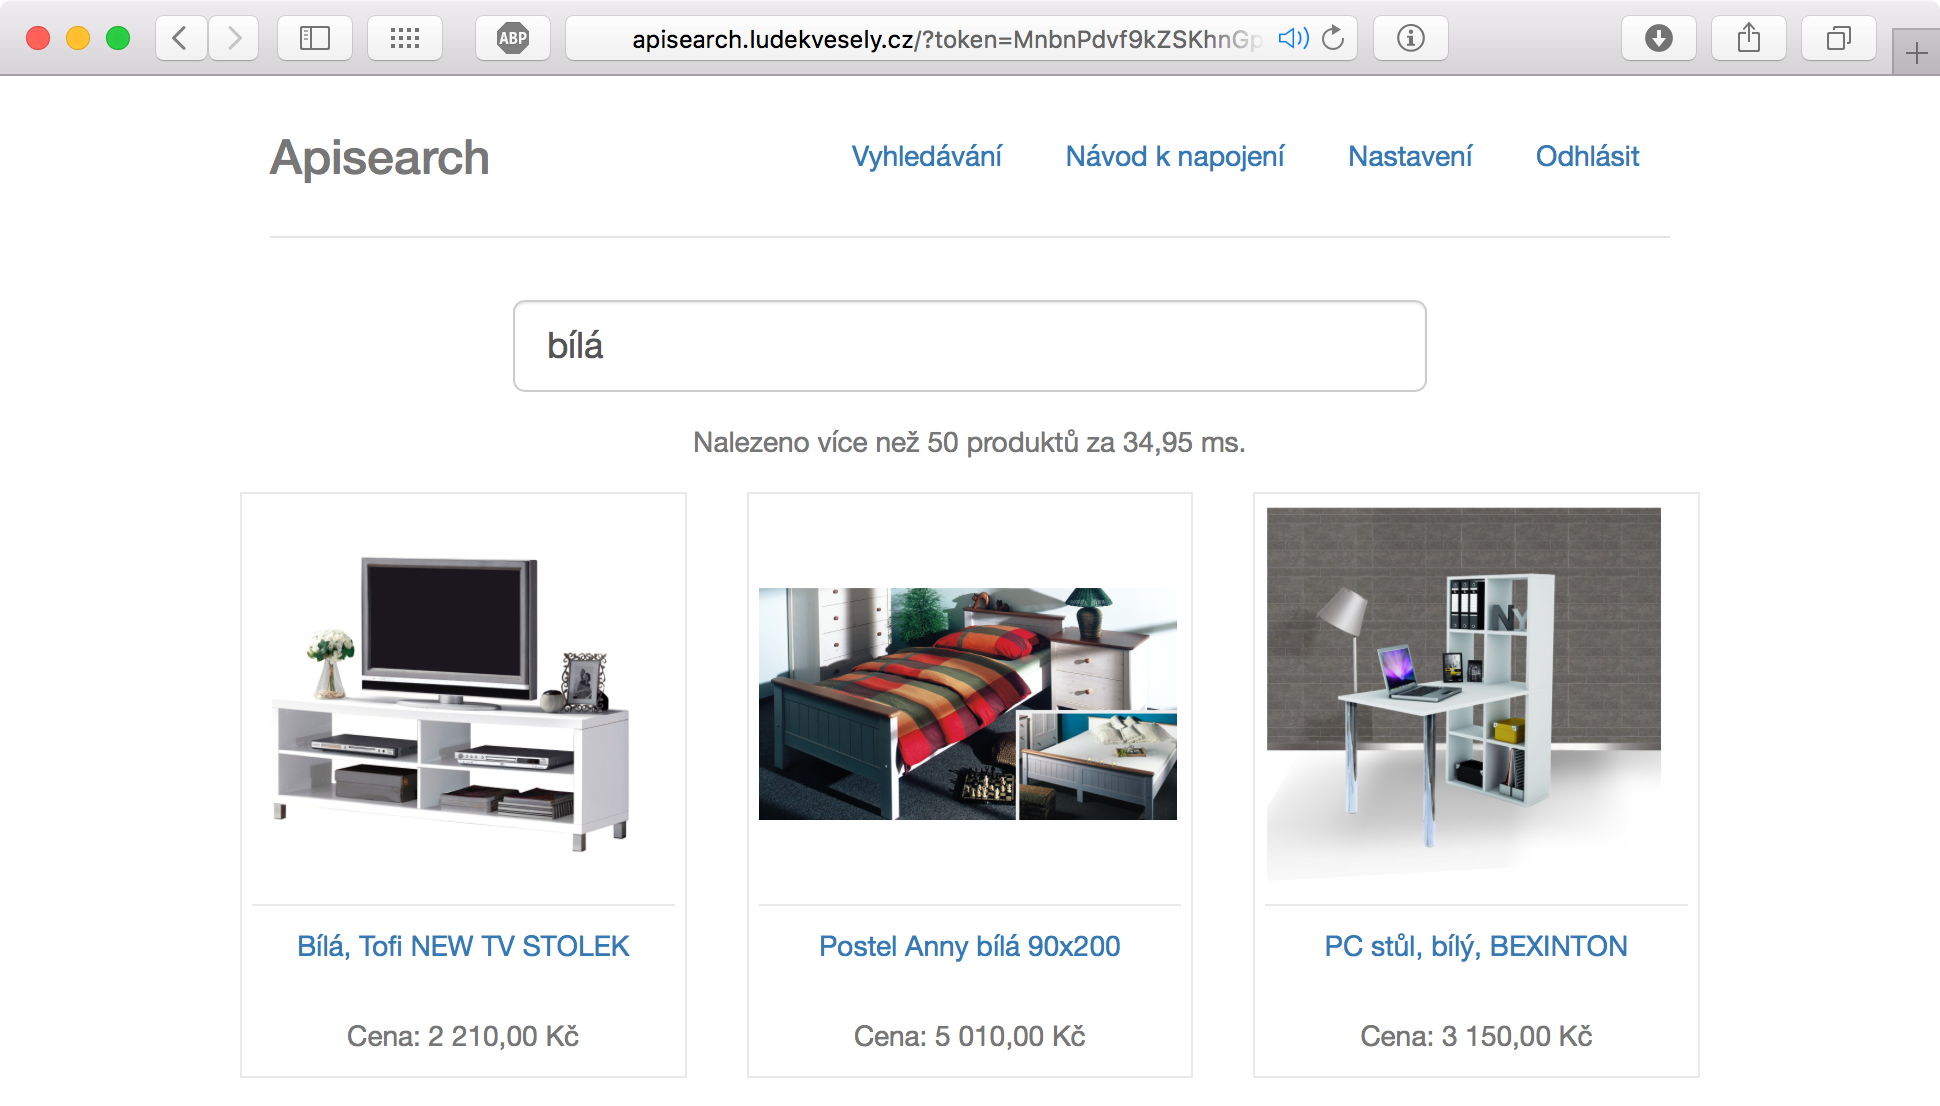
\includegraphics[width=\textwidth]{frontend.png}
\caption{Frontend -- kontrola funkce vyhledávání}
\label{frontend}
\end{figure}

Dále je součástí této aplikace návod na napojení elektronického obchodu. To je popsáno jednak
principiálně (s odkazem na dokumentaci v Apiary), tak je k dispozici příklad implementace, 
který je možné rovnou zkopírovat do webu obchodu. Příklady jsou pro nejpoužívanější jazyky
z prostředí webu (PHP a JavaScript), přičemž jsou navrženy tak, aby nebylo třeba instalovat
další závislosti a napojení tak bylo co nejsnadnější.

Poslední možností, kterou aplikace nabízí je úprava nastavení -- uživatel zde může změnit
přihlašovací údaje (e-mail nebo heslo) a adresu XML souboru s produkty. Z aplikace se může 
uživatel odhlásit, veškeré jeho nastavení je dostupné pouze po přihlášení, což je nutné
pro možnost využívání aplikace více uživateli (elektronickými obchody).

\section{Backend}

Dále je třeba rozhodnout, v čem bude psán backend, pomocí jakého programovacího jazyka
nebo frameworku. Možností je celá řada, v úvahu přichází jak využití dynamických skriptovacích 
jazyků běžně využívaných pro web (nejpoužívanější PHP nebo JavaScript), přes jazyky 
s~komplexnějším prostředím využívající k běhu virtuální stroj (Java, .NET), až po statické 
překládané jazyky (C, C++, GoLang). Je třeba zvolit takový jazyk, který bude rozumně použitelný, 
bude k němu dostatek knihoven pro tvorbu API a práci s Elasticsearch, aby netrvala samotná
implementace neúměrně dlouho. Na druhou stranu je však třeba, aby daný jazyk umožňoval
vytvoření serveru, který bude schopný vyřizovat požadavky co nejrychleji.

Vzhledem k požadované rychlosti nepřichází v úvahu skriptované jazyky, které sice mohou
poskytovat rozumnou dobu odezvy, pokud je ale možnost ji snížit pomocí jiného jazyku, 
není důvod toho nevyužít. Volba padla na jazyk GoLang, což je jazyk, který vznikl 
ve společnosti Google a měl přinést některé výhody dynamicky typovaných jazyků do jazyků 
staticky typovaných \cite{go-in-action}. Přináší zejména stručný zápis některých konstrukcí, 
snadný a rychlý překlad. 
Součástí distribuce SDK je také balíčkovací manažer, nástroje pro formátování zdrojových kódů, 
statickou analýzu nebo dokumentaci.
GoLang disponuje knihovnami pro implementaci API, HTTP serveru i komunikace s Elasticsearch. Nebrzdí 
také případné další rozšiřování, je možné s jeho pomocí implementovat podporu dalších protokolů jako
WebSockets nebo gRPC. Zároveň však téměř odstraňuje nevýhody jazyků vyžadující překlad.
Samotný překlad je velmi rychlý, v řádu jednotek sekund, což je ve srovnání s ostatními
jmenovanými jazyky výrazně rychlejší. Dálší výhodou je, že po překladu vznikne jeden
binární soubor, který nevyžaduje žádné běhové prostředí a není závislý na jiných knihovnách, 
což výrazně zkrátí dobu sestavení i nasazení.

Pro zpracování spuštění programu z příkazové řádky je použita knihovna \verb|urfave/cli|, 
která umožňuje definovat jednotlivé argumenty, s nimiž může být aplikace spuštěna.
Obsahuje také sadu základních příkazů jako je zobrazení nápovědy nebo verze programu.
V této aplikaci jsou definovány celkem tři příkazy -- spuštění serveru, spuštění asynchroního
importu produktů a vytvoření indexu v Elasticsearch.

\begin{code}
\captionsetup{singlelinecheck=false,justification=raggedright}
\captionof{listing}{Struktura produktu v jazyce Go}
\label{code:go-product}
\begin{minted}{go}
type Product struct {
    Id          string `xml:"ITEM_ID" json:"id"`
    UserId      string `xml:"-" json:"userId"`
    Name        string `xml:"PRODUCTNAME" json:"name"`
    Description string `xml:"DESCRIPTION" json:"description"`
    Url         string `xml:"URL" json:"url"`
    Img         string `xml:"IMGURL" json:"img"`
    Price       int    `xml:"PRICE_VAT" json:"price"`
    Updated     string `xml:"-" json:"updated"`
}
\end{minted}
\end{code}

Vytvoření indexu je možné spuštěním přeloženého programu s argumentem \verb|createIndex|.
Po spuštění je spuštěna funkce \verb|CreateIndex| v balíčku \verb|elastic|. 
Ta vytvoří indexy v Elasticsearch (pokud neexistují) a následně u nich aktualizuje mapování.
Lze tak tento příkaz použít pro přidávání nových polí i v produkčním prostředí.

\begin{code}
\captionsetup{singlelinecheck=false,justification=raggedright}
\captionof{listing}{Hromadná indexace produktů}
\label{code:go-indexing}
\begin{minted}{go}
// Vytvoření procesoru pro hromadný import
bulk, err := products.BulkStart()
// Indexace každěho produktu
for i, _ := range productList.ProductList {
    productList.ProductList[i].UserId = s.UserId
    productList.ProductList[i].Updated = time.Now().Format("2006-01-02T15:04:05-07:00")
    productList.ProductList[i].BulkIndex(bulk)
}
// Dokončení indexace - uložení zbývajících produktů a zavření procesoru
err = products.BulkFlush(bulk)
\end{minted}
\end{code}

Druhým příkazem je spuštění importu produktů po spuštění programu s argumentem \verb|import|.
To je vykonáno spuštěním funkce \verb|ImportXmlFiles| v balíčku \verb|importer|. Ta načte 
veškeré konfigurace uživatelů a pro každou z nich spustí import produktů prostřednictvím 
funkce \verb|ImportXmlFile|. Pro samotnou komunikaci s Elasticsearch je použita knihovna 
\verb|olivere/elastic|. Import produktů je implementován tak, že se nejprve načte zdrojový
XML soubor, který se namapuje na pole produktů pomocí vestavené
funkce \verb|Unmarshal| \cite{go-xml}. Produkt je zde struktura, která je definována 
ve výpisu \ref{code:go-product}.

Součástí definice struktury není pouze výpis jejích prvků s odpovídajícími datovými typy, 
ale také nastavení pro převod struktury do textového řetězce ve formátu XML a JSON.
Každý produkt který vznikl převodem z XML je následně převeden s pomocí interní funkce \verb|Marshall|
na textový řetězec ve formátu JSON. To už je formát, ve kterém může být produkt ukládán do
Elasticsearch. Ukládání produktů je provedeno pomocí hromadné indexace.

\begin{code}
\captionsetup{singlelinecheck=false,justification=raggedright}
\captionof{listing}{Routování HTTP serveru}
\label{code:go-routing}
\begin{minted}{go}
route := Route{
    "Search",                          // Nazev
    "GET",                             // HTTP metoda
    "/api/v1/search/{userId}/{query}", // Vzor URL
    v1.Search,                         // Obslužná funkce
    []string{},                        // Validace argumentů URL
}
\end{minted}
\end{code}

Ta je na pozadí implementována tak, že ukládání probíhá paralelně a navíc Elasticsearch 
provádí samotnou indexaci v dávkách. Díky tomu je import extrémně rychlý a přitom 
není třeba se starat o spouštění dalších procesů -- to provádí knihovna s pomocí
příkazu \verb|go| \cite{go-concurrency}.

Poslední možností jak přeložený program spustit je nastartování HTTP serveru. Server
je použit z standardní knihovny \verb|net/http|. Pro routování příchozích požadavků
na odpovídající funkce na základě použité URL je použita knihovna \verb|gorilla/handlers|.
Každý možný tvar požadavku je definován jako struktura:

Toto je konkrétní zápis definice koncového bodu pro vyhledávání v produktech daného uživatele.
Požadavek poté obsloužen funkcí, která má v tomto případě předpis 
\verb|func Search(w http.ResponseWriter, r *http.Request) {}|. Může tedy číst veškeré
parametry s nimiž byla spuštěna (\verb|*http.Request|) a také má kam zapsat
výstup, ať už se jedná o odpověď ve formátu JSON nebo odpovídající stavové kódy 
(\verb|http.ResponseWriter|). Uvnitře této funkce je provedeno samotné vyhledávání
pomocí funkce \verb|products.Search|, která vrací pole produktů. Ty jsou následně transformovány
do formátu JSON a vráceny jako odpověď serveru.

\section{Nasazení aplikace do produkčního prostředí}

\begin{figure}[h]
\center
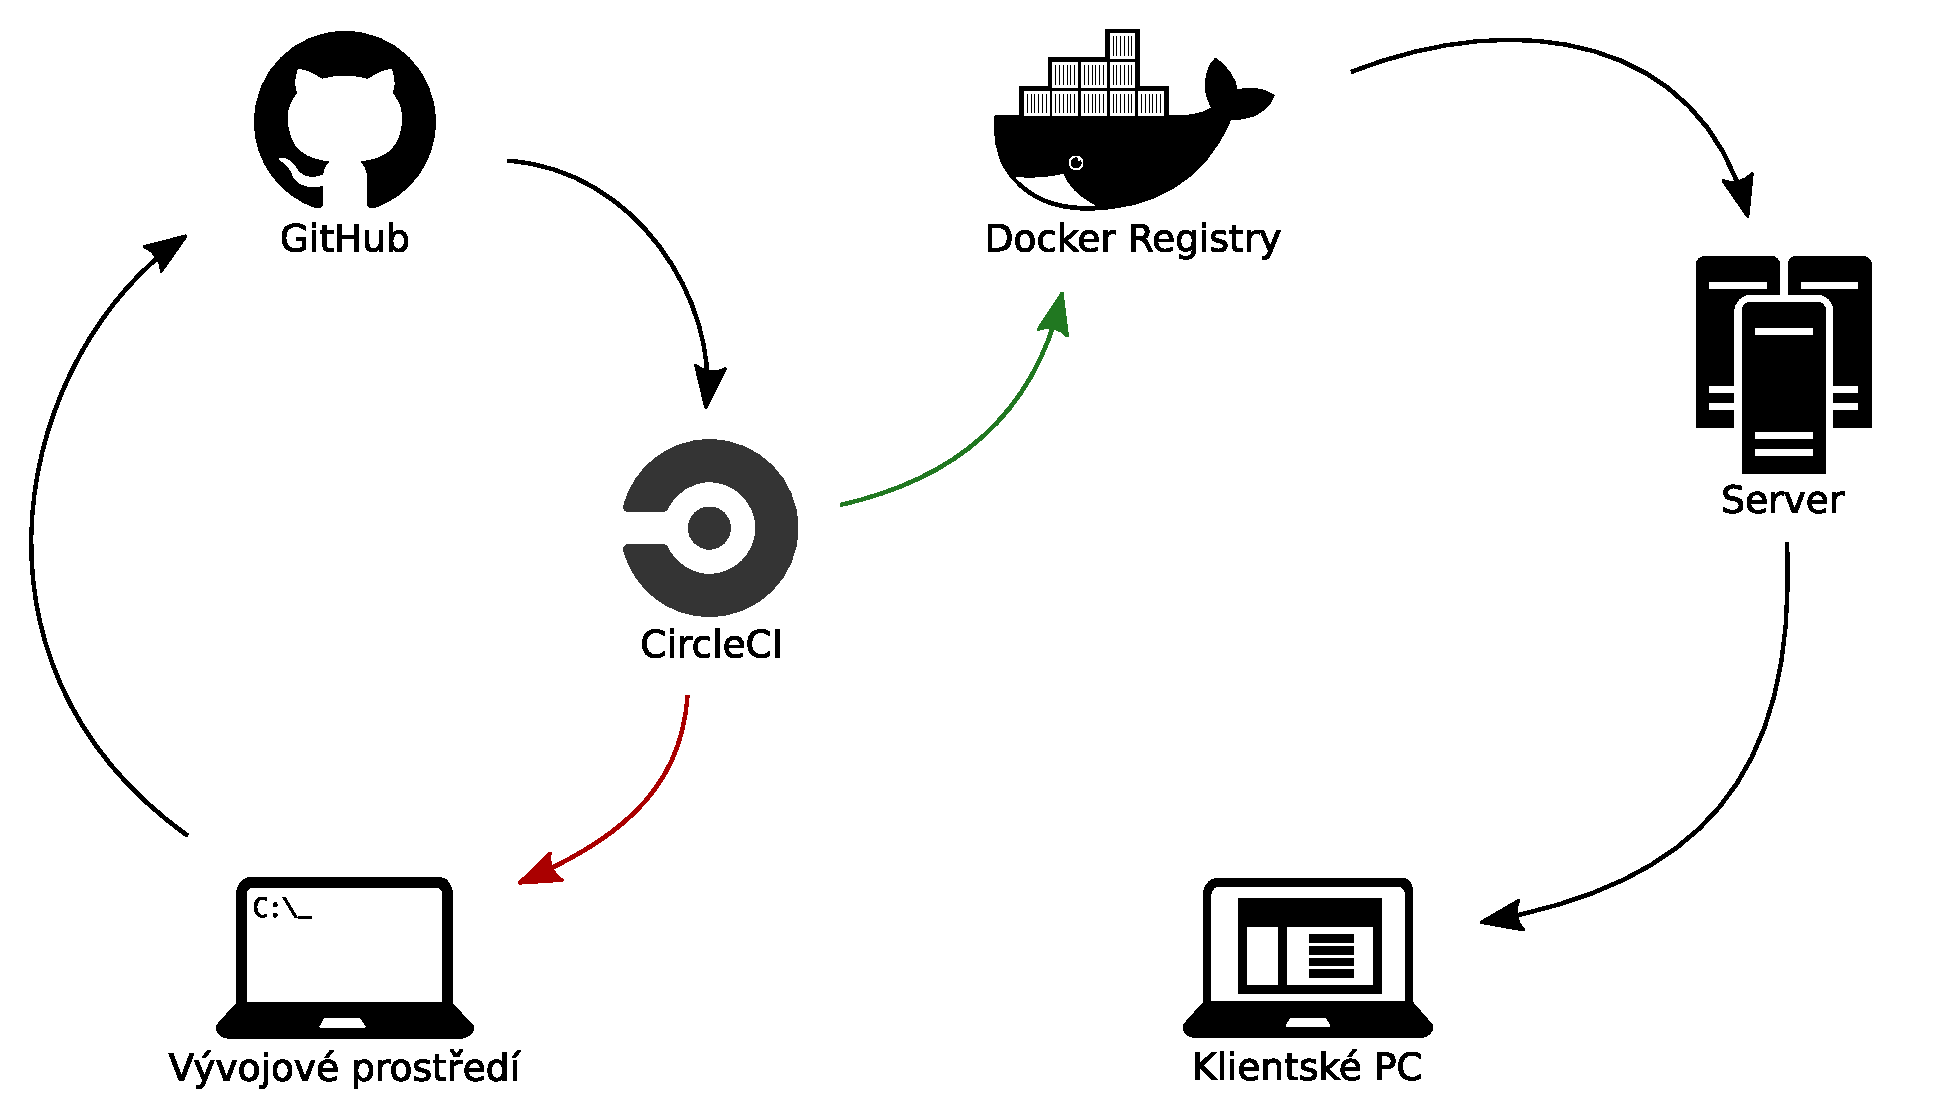
\includegraphics[width=\textwidth]{circleci.pdf}
\caption[Kontinuální nasazování aplikace]{Kontinuální nasazování aplikace pomocí CircleCI (Zdroj: \cite{circleci})}
\label{circle-ci}
\end{figure}

Posledním krokem k zveřejnění aplikace a jejímu zpřístupnění veřejnosti je její nasazení 
do produkčního prostředí. Pro vytvoření nasaditelného artifaktu je použit nástroj Docker, 
obdobně jako při distribuci Elasticsearch. Aby nemusel vývojář po každé změně zdrojových
kódů znovu ručně vytvářet a nasazovat novou verzi aplikace (což je zdlouhavé a navíc může
vést k chybám \cite[strana~23]{devops}), je vzdálený GIT repozitář propojen s integračním 
serverem, který provede sestavení a nastavení aplikace automaticky. Konkrétně je používán 
CircleCI \cite{circleci}.

Pomocí CircleCI je nasazován jak frontend, tak backend. Vývojář nahraje provedené změny
v lokálním repozitáři do repozitáře vzdáleného (GitHub), ten poté odešle požadavek do
napojeného integračního serveru (CircleCI) s informací o repozitáři, který byl aktualizován.
V rámci CircleCI je spuštěn nový virtuální stroj, který stáhne aktuální verzi zdrojových kódů
z vzdáleného repozitáře a dále postupuje podle příkazů definovaných v souboru \verb|circle.yml|.
V něm je definováno jak mají být získány závislosti aplikace (příkazem \verb|go get| v případě 
backendu) a jak má být aplikace sestavena (\verb|go build| v případě backendu). Vytvořený binární
soubor je poté nakopírován do prázdného Docker obrazu, který je poté spuštěn příkazem \verb|docker run|. 
Tím je ověřeno, že byl obraz sestaven v pořádku a je nahrán do registru příkazem \verb|docker push|.
Nakonec je spuštěno samotné nasazení, které je provedeno pomocí nástroje \verb|docker-compose|
na vzdáleném serveru.

Všechny kontejnery jsou spravovány prostřednictvím nástroje Docker Compose \cite{compose}.
Ten usnadňuje práci s Docker démonem -- používá vlastní sadu příkazů a veškerá konfigurace
se provádí pomocí YAML souboru. Díky tomu, že jde o deklarativní přístup, je možné
příkazy opakovat a vždy je dosaženo stejného očekávaného výsledku. Tento konfigurační 
soubor je pojmenován \verb|docker-compose.yml| a má pro tuto aplikaci podobu zobrazenou 
ve výpisu \ref{code:docker-compose}.

\begin{code}
\captionsetup{singlelinecheck=false,justification=raggedright}
\captionof{listing}{Konfigurace pro Docker Compose}
\label{code:docker-compose}
\begin{minted}{yaml}
web-admin:
  image: apisearch/web-admin
  ports:
   - "7010:8080"
  links:
   - apisearch
  restart: always
apisearch:
  image: apisearch/apisearch
  command: server
  ports:
   - "7011:8080"
  links:
   - elasticsearch
  restart: always
elasticsearch:
  image: apisearch/elasticsearch
  volumes:
   - /mnt/apisearch/elasticsearch:/usr/share/elasticsearch/data
  restart: always
\end{minted}
\end{code}

Tento soubor definuje takzvaný stack, což je skupina několika souvisejících služeb. V tomto
případě jsou definovány tři služby (\verb|web-admin| -- frontend, \verb|apisearch| -- backend 
a \verb|elasticsearch|). U všech služeb je nastaveno, aby se v případě chyby automaticky restartovaly.
Dále je u prvních dvou služeb definován port, přes který jsou dostupné. Na serveru je pak 
nastavena proxy, která na základě celé URL směruje příchozi požadavky na jednu z těchto služeb.
U služby \verb|elasticsearch| je v \verb|volumes| definována složka, do které jsou persistována
data. Po restratu kontejneru totiž dochází ke ztrátě jeho dat, což by byl problém vzhledem
k stavovosti služby. Je tedy zvolena složka v hostitelském stroji, která je použita pro persistenci
těchto dat. Celou skupinu služeb je možné spustit jediným příkazem \verb|docker-compose up -d|.
Zároveň je možné pomocí tohoto nástroje sledovat logy všech běžících služeb, jejich stav
a případně je aktualizovat nebo zastavovat.

Použití tohoto nástroje má výhodu v tom, že vzhledem k tomu, že jej oficiálně vydává Docker, 
v dobré podpoře a kompatibilitě s ostatními nástroji. V případě nutnosti horizontálního škálování
lze využít některý z orchestrátorů \cite[strana~300]{devops} (například Docker Swarm, Docker Cloud 
nebo Rancher), které jsou s tímto formátem zápisu kompatibilní. 

% TODO: monitoring, logovani

\chapter{Testování, ověření funkčnosti}

V této kapitole jsou popsány proběhlé testy, kterými je ověřeno splnění požadavků na aplikaci
a tedy odpovídající přínos vzniklé aplikace. Testy jsou rozděleny do tří skupin. Nejprve jsou
ověřeny splněné funkční požadavky, tedy požadavky na samotné vyhledávání. Testování je
prováděno na reálných datech, je ověřováno, jak se vyhledávání vyrovnává s tvaroslovím 
nebo neúplným zadáním hledaného výrazu. Dále je testována rychlost odezvy běžící služby, 
kdy je po určitou dobu systém vystaven soustavné zátěži a je pozorována doba, za kterou jsou 
požadavky vyřízeny. Nakonec je testována snadnost napojení, což je provedeno formou demonstrace
provedení napojení na konkrétním elektronickém obchodě.

\section{Testovací data}

Jako testovací data jsou použity produkty obchodu s nábytkem. Ty jsou uloženy jako XML soubor
ve formátu Heuréka.cz, jehož struktura je znázorněna ve~výpisu~\ref{code:xml-heureka}. Celkem
tento soubor obsahuje kompletní informace o 3732 produktech. Tento XML soubor je k~dispozici
na přiloženém CD ve složce \verb|/src/docker-stack/data|, kde je připravena jak varianta obsahující
všechny produkty, tak varianta s dvěma produkty pro účely testování funkčnosti importu.

\section{Snadnost napojení na službu}

Přestože by dávalo smysl nejprve otestovat samotnou funkčnost vyhledávání, je v tuto chvíli jako
první testována snadnost napojení na službu. Na konci tohoto testu je vytvořen nový účet s importovanými
daty, což lze použít pro provedení dalších testů.

Uživatel provádějící napojení nejprve přejde na web aplikace (dostupné pod URL \url{https://apisearch.ludekvesely.cz}), 
kde provede registraci se svou e-mailovou adresou a zvoleným heslem. Zároveň je třeba zadat URL, pod
kterou je k dispozici XML soubor s produkty.

Po odeslání formuláře je uživateli vytvořen účet, je uloženo zadané nastavení a na pozadí je spuštěn
import produktů z zadaného souboru. Uživateli je toto zobrazeno informativní hláškou a je mu zobrazena
stránka s formulářem pro vyzkoušení vyhledávání. Zároveň jsou v produktech nalezeny často se objevující
výrazy, které jsou uživateli doporučeny pro vyhledání, uživatel tedy vidí jediné vstupní pole s nápovědou, 
může tedy bez váhání zkoušet práci s vyhledáváním, prohlížet si výsledky a kontrolovat dobu vyhledávání.

Pokud je uživatel s vyhledáváním spokojen, může začít s napojením, poté co přejde na záložku 
\textbf{Návod k~napojení}, je mu zobrazen obecný princip funkce API i příklady implementace v konkrétních
programovacích jazycích, což je vidět na obrázku \ref{connection}.

\begin{figure}[h]
\center
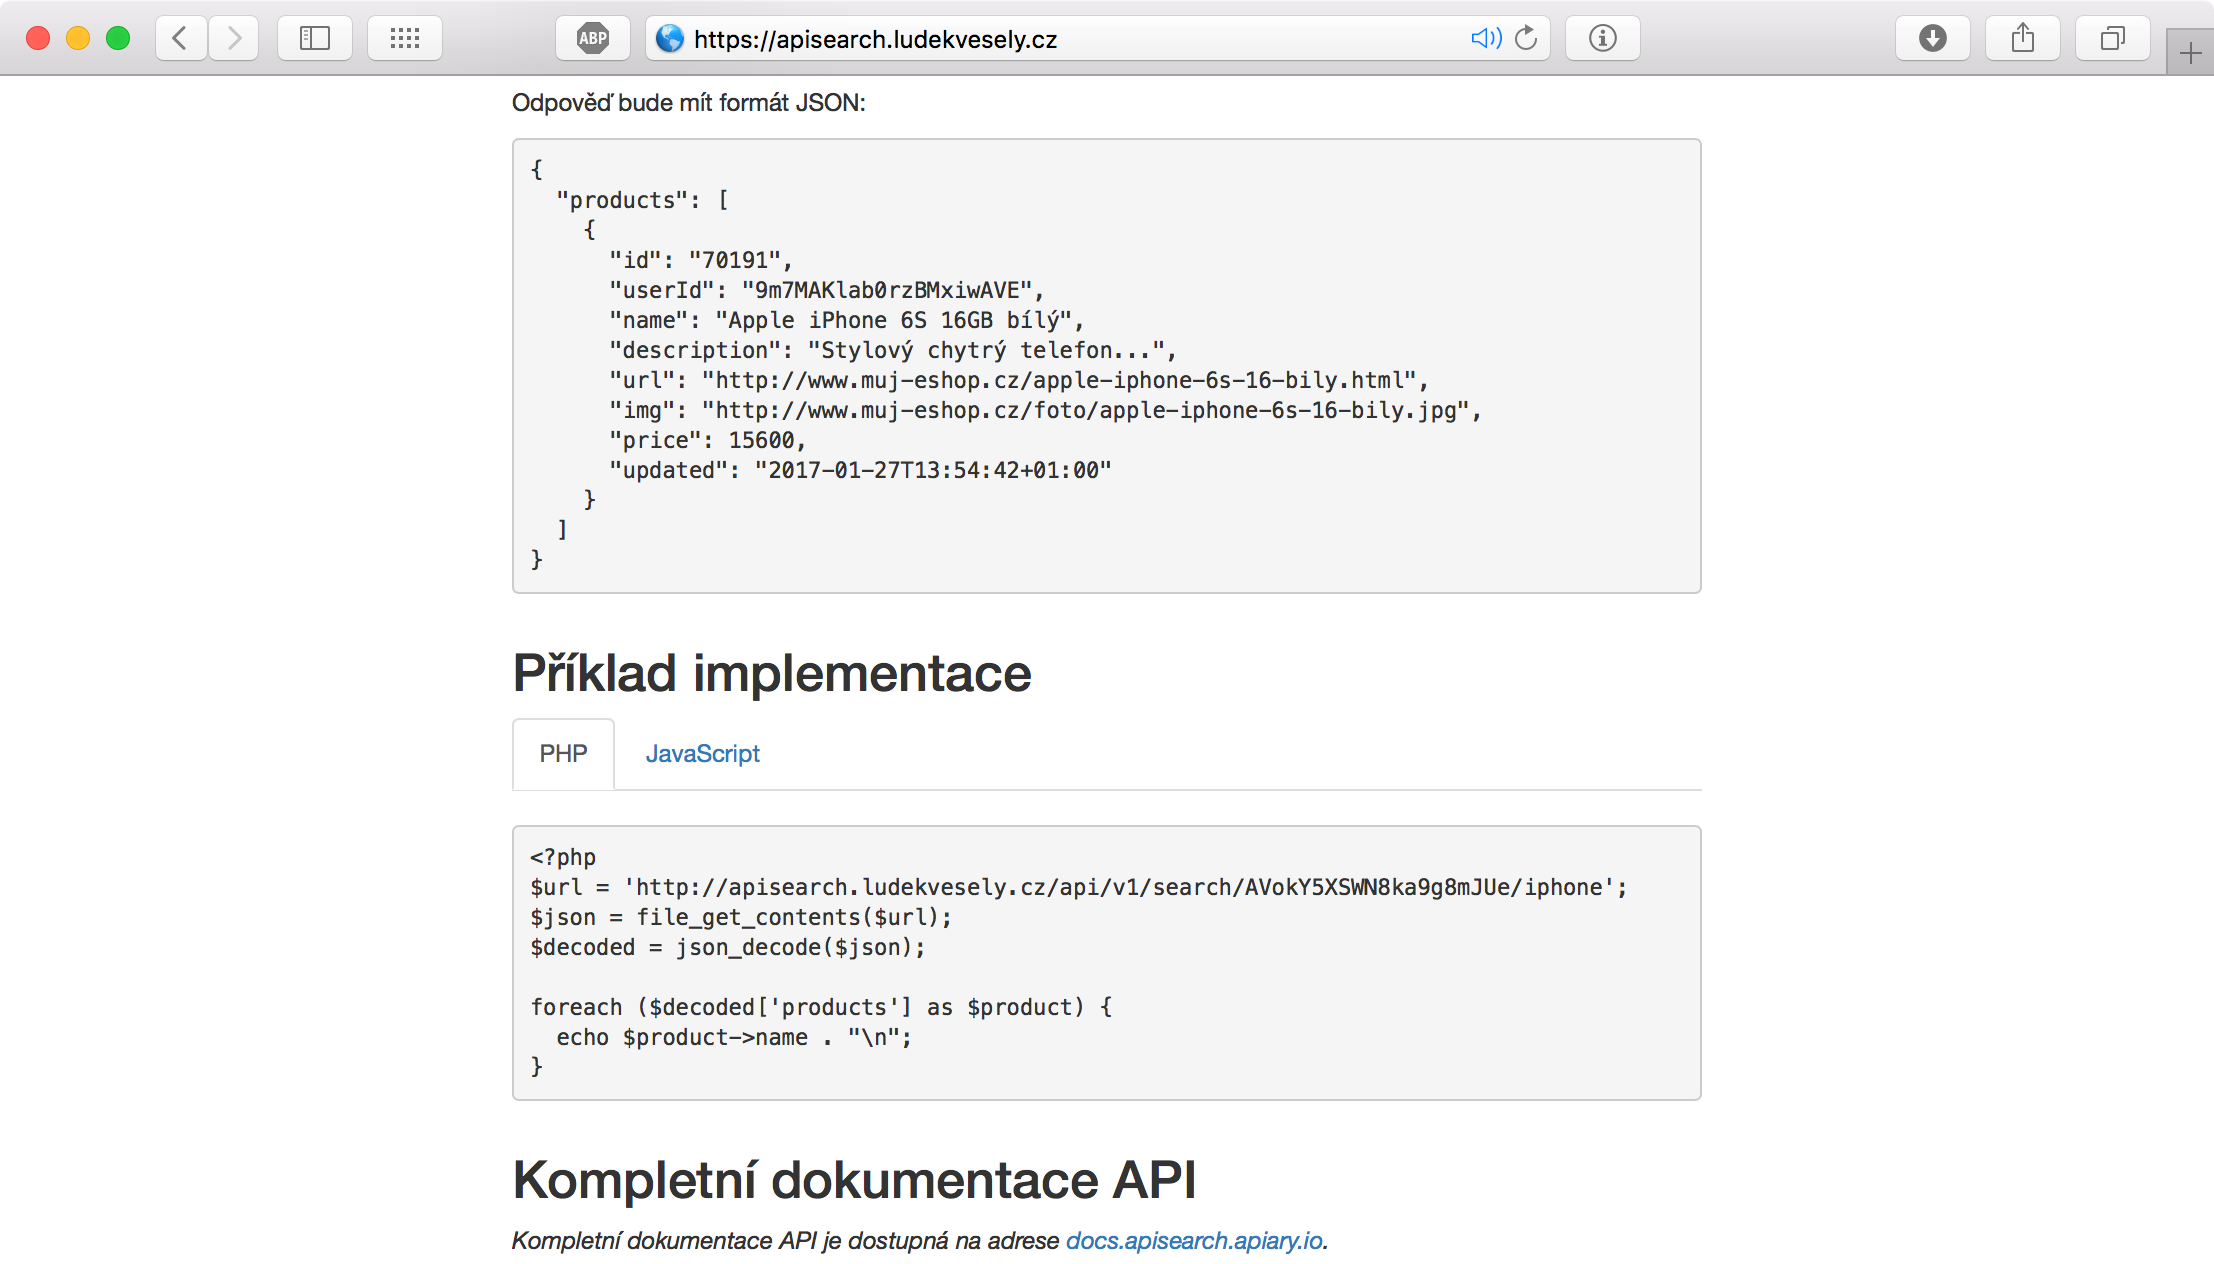
\includegraphics[width=\textwidth]{napojeni.png}
\caption{Manuál pro napojení na službu}
\label{connection}
\end{figure}

Uživatel rovnou vidí i formát, v jakém obdrží odpověď a jak s ní pracovat v daném programovacím jazyce.
Samotná implementace tedy spočívá v nahrazení části kódu elektronického obchodu, která se stará o~vyhledání 
produktů v databázi právě nabízeným kódem. Celý tento postup je k dispozici jako video v příloze této práce
a samotná konfigurace služby zabere maximálně několik minut, doba implementace na straně obchodu se již může
lišit dle způsobu, jakým web k produktům přistupuje a jakým stylem je programována.

Dále je zde uveden odkaz na kompletní dokumentaci dostupnou online prostřednictvím služby Apiary.
Tu může využít pro případnou obsluhu nástroje z jeho aplikace, toto užití však nebude pravděpodobně
hojně využíváno, protože jde proti principu jednoduchého a rychlého napojení.

\section{Funkčnost vyhledávání}

Dále testuji funkčnost vyhledávání, tedy to, jak si nástroj poradí s jednotlivými problémy 
definovanými v~kapitole \ref{ch:pozadavky-vyhledavani}. Celý test je možné provést spuštěním
skriptu \verb|test-search-results.php|. Ten pro každý uložený výraz provede hledání, 
obdrženou odpověď dekóduje a vypíše názvy prvních odpovídajících produktů.

Nejprve je testováno vyhledání dle přesné shody názvu produktu \verb|Matrace Sofia|. Dále
je vyhledán textový řetězec, který v dané databázi neexistuje a neměl by tedy vést k nalezení
žádného produktu.

\begin{code}
\captionsetup{singlelinecheck=false,justification=raggedright}
\captionof{listing}{Test vyhledávání -- přesná shoda, neexistující výraz}
\label{code:search-exact}
\begin{minted}{text}
+-----------------------------------------------------------------+
| query: 'Matrace Sofia'                                    33 ms |
+-----------------------------------------------------------------+
| Matrace Sofia                                                   |
| postel Sofia 180x200 doprava + rošt zdarma                      |
| Sedací souprava, rohová P, rozkládací, ekokůže bílá/šenil š...  |
| Sedací souprava, rohová P, rozkládací, ekokůže černá/šenil ...  |
+-----------------------------------------------------------------+
+-----------------------------------------------------------------+
| query: 'lednička'                                         12 ms |
+-----------------------------------------------------------------+
| --- not found ---                                               |
+-----------------------------------------------------------------+
\end{minted}
\end{code}


Ve výpisu \ref{code:search-exact} je nejprve nalezen produkt, jehož název přesně odpovídá zadanému 
výrazu. Dále jsou nalezeny produkty obsahující název \verb|Sofia|. Nabízí se otázka, proč nejsou
nejdříve zobrazeny všechny produkty odpovídající slovo \verb|matrace|. Důvod je ten, že v kompletní
databázi je toto slovo výrazně častější, což dle vztahu \ref{tfidf} vede k~vzniklému pořadí.
V praxi je výsledek ten, že jsou nejprve zobrazeny produkty patřící do dané produktové řady
a až následně produkty méně související s hledaným produktem.

Následně je hledáno podle jiného tvaru slova, kdy je v~hledáném výrazu uvedeno slovo v~jiném 
pádu (\verb|matrací|) než v názvu produktu (\verb|matrace|). V tomto případě je očekáváno, že budou 
nalezeny produkty obsahující dané slovo v jiném tvaru. Ve výsledcích \ref{code:search-morpf} je vidět, 
že byly skučeně nalezeny produkty, které byly pravděpodobně hledány -- matrace. Zároveň je tento 
příklad kontrola toho, že je možné vyhledávat nezávisle na velikosti písmen.

\begin{code}
\captionsetup{singlelinecheck=false,justification=raggedright}
\captionof{listing}{Test vyhledávání -- přesná shoda, neexistující výraz}
\label{code:search-morpf}
\begin{minted}{text}
+-----------------------------------------------------------------+
| query: 'matrací'                                          19 ms |
+-----------------------------------------------------------------+
| Matrace Neapol                                                  |
| Matrace Riviera                                                 |
| Matrace Sofia                                                   |
| Matrace Bára                                                    |
+-----------------------------------------------------------------+
\end{minted}
\end{code}

Další disciplínou je našeptávání produktů, tedy vyhledávání v~okamžiku, kdy ještě není specifikovaný
celý hledaný výraz. Při hledání prvních několika písmen je to obtížné, máloky bude vystihnuto, co
měl zákazník na mysli. S rostoucím počtem písmen nebo dokonce slov by se však měla přesnost zlepšovat.
Ve výpisu \ref{code:search-suggest} je vidět, že v prvním případě jsou produkty \verb|MATRAC| ve výsledcích
dříve, což sice poukazuje na překlep v názvu produktu, nicméně takové chování je v pořádku.
Toto slovo je totiž "podobnější" zadanému výrazu, liší se jen o jeden znak, narozdíl od slova
\verb|Matrace|, které je o znak delší a tudíž se liší o dva znaky (bez ohledu na velikost písmen).

\begin{code}
\captionsetup{singlelinecheck=false,justification=raggedright}
\captionof{listing}{Test vyhledávání -- našeptávání}
\label{code:search-suggest}
\begin{minted}{text}
+-----------------------------------------------------------------+
| query: 'matra'                                            32 ms |
+-----------------------------------------------------------------+
| MATRAC MONTANA 80x190x9 cm                                      |
| Matrac, gumotex, 200x80 cm, MONIKA                              |
| Matrace Riga 1+1 zdarma                                         |
| Matrace Neapol                                                  |
+-----------------------------------------------------------------+
+-----------------------------------------------------------------+
| query: 'matrace ma'                                       20 ms |
+-----------------------------------------------------------------+
| Matrace Maxi                                                    |
| Matrace Maxi Kings                                              |
| Matrace Neapol                                                  |
| Matrace Riviera                                                 |
+-----------------------------------------------------------------+
\end{minted}
\end{code}

Dále je testováno, jak se dokáže aplikace vyrovnat s překlepy při formulaci dotazu na vyhledávání.
Vzhledem k nastavené editační vzdálenosti rovnou jedné je tolerována jediná změna, tedy vložení, změna
nebo odebrání jediného znaku ve výrazu. 

\begin{code}
\captionsetup{singlelinecheck=false,justification=raggedright}
\captionof{listing}{Test vyhledávání -- našeptávání}
\label{code:search-fuzzy}
\begin{minted}{text}
+-----------------------------------------------------------------+
| query: 'matrXce'                                          21 ms |
+-----------------------------------------------------------------+
| Matrace Neapol                                                  |
| Matrace Riviera                                                 |
| Matrace Sofia                                                   |
| Matrace Bára                                                    |
+-----------------------------------------------------------------+
\end{minted}
\end{code}

Nakonec zbývá otestovat práci se synonymi. Ve slovníku je definováno pro slovo \verb|police| synonymum
\verb|polička|. Je tedy testován výraz obsahující slovo, přičemž se očekává, že budou ve výsledcích obě
slova zastoupena rovnocenně, tedy budou nalezeny jak police, tak poličky. Rozdíl v těchto slovech
je velký na to, aby to bylo pokryto zpracováním překlepů, nahrazení synonym je tedy jediný způsob, 
jak tohoto chování docílit.

Tímto byly otestovány požadavky kladené na vyhledávání při definici řešeného problému. 
Nelze však předvídat, jaké všechny výrazy budou koncoví uživatelé vyhledávání zadávat do 
vyhledávání. Je tedy třeba po nasazení do ostrého provozu analyzovat proběhlá vyhledávání a
zaměřit se tak na opakující se vyhledávání nebo na vyhledávání jež nevedou k prokliku, což
může být indikátor toho, že aplikace uživateli nenabídla to, co hledal. Tuto práci
bude jistě možné automatizovat a dosahovat tak lepších výsledků průběžněji.

Při úpravách vyhledávacího algoritmu poté nesmí být opomenuto spouštění stávajících testů, 
aby nebyly do systému zavlečeny chyby namísto požadovaného zlepšení vyhledávání. Zároveň
je však třeba testy rozšiřovat o kontrolu nové funkcionality, aby nebyly zastaralé.

\begin{code}
\captionsetup{singlelinecheck=false,justification=raggedright}
\captionof{listing}{Test vyhledávání -- synonyma}
\label{code:search-synonym}
\begin{minted}{text}
+-----------------------------------------------------------------+
| query: 'polička šedá'                                     23 ms |
+-----------------------------------------------------------------+
| Police, šedá, LOBETE 01                                         |
| Police, šedá, PIERE P11                                         |
| Police, šedá, DIDO                                              |
| Police, šedá, LUPO                                              |
+-----------------------------------------------------------------+
\end{minted}
\end{code}

\section{Rychlost služby}

V okamžiku, kdy jsou do aplikace uloženy produkty je možné otestovat také její rychlost. Testu je 
podroben pouze koncový bod pro provádění vyhledávání, u dalších není rychlost tak kritická jako v tomto
případě. Ten má podobu \verb|/api/v1/search/{userId}/{query}|. I když při testování funkčnosti vyhledávání
bylo dosahováno odpovídajících časů odezvy, v praxi je aplikace používána více uživateli, kteří
provádí více vyhledávání v kratších intervalech -- po každém stisku klávesy.

Testování probíhá tak, že je načten soubor definující URL, na které jsou vznášeny požadavky.
Následně jsou tyto požadavky po určitou dobu opakovány a u každého je uložena doba, která byla 
potřebná pro jeho vyřízení. Toto celé je spuštěno paralelně v několika vláknech, což simuluje 
právě použití více uživateli. 

Pro takové testování je třeba vybrat nástroj, který umí načíst zadaný seznam URL a
ty následně v~několika vláknech otestovat. Výstupem by měl být jak průměrný čas vyřizování
požadavků, tak také přehledná vizualizace proběhlého testování. Pro tento účel by bylo
možné použít nástroj \verb|ab| \cite{ab}, který je snadno instalovatelný a jeho použití
je triviální -- lze jej spustit s parametry značícími požadovaný počet provedených požadavků, 
počet paralelních vláken, v nichž je test prováděn a URL, která je testována. Problém je však 
v podpoře jediné testované URL, což by bylo možné řešit spuštěním více procesů s různými 
argumenty na pozadí. Větší je však problém s vizualizací výsledků testů. Lze sice vytvořit 
vizualizaci s pomocí nástroje \verb|gnuplot|, jeho použití však není příliš intuitivní.

\begin{code}
\captionsetup{singlelinecheck=false,justification=raggedright}
\captionof{listing}{Spuštění zátěžových testů}
\label{code:sniper}
\begin{minted}{text}
> sniper -c 10 -n 1000 -f urls.txt
This is Sniper, version 1.0, copyright (C) 2013 by Lubia Yang.

The server is now under snipe ...

Transactions:                   1000 hits
Availability:                   100.00 %
Elapsed time:                   7.32 secs
Document length:               48582 Bytes
TotalTransfer:                 46.33 MB
Transaction rate:             136.67 trans/sec
Throughput:                     6.33 MB/sec
Successful:                     1000 hits
Failed:                           0 hits
TransactionTime:              72.978 ms(mean)
ConnectionTime:                0.200 ms(mean)
ProcessTime:                  72.778 ms(mean)
StateCode:                    1000(code 200)
\end{minted}
\end{code}

Z toho důvodu je použit nástroj \verb|sniper| \cite{sniper}, který funkčnost nástroje \verb|ab|
rozšiřuje o podporu více URL i o možnost přímého generování reportů. Ukázka spuštění je ve~výpisu 
\ref{code:sniper}. Příkaz je spuštěn s parametry \verb|-c|, který značí počet použitých vláken a 
\verb|-n|, což definuje počet provedených požadavků, po nichž je testovýní ukončeno. V souboru 
\verb|urls.txt| jsou pak uloženy URL, na které jsou prováděny požadavky, přičemž každý z nich je 
uložen na jednom řádku tohoto textového souboru.

Po spuštění příkazu je zobrazen průběh testování a celkové statistiky proběhlých testů. Kromě
toho je vygenerován graf, který je možné otevřít ve webovém prohlížeči a prohlížet tak dobu 
odezvy v~průběhu času. V tomto konkrétním spuštění je \textbf{průměrná doba odezvy 72 ms}.
To je sice výrazně více ve srovnání se samostatně probíhajícím vyhledávání v předchozí kapitole, 
stále to však splňuje požadavek na rychlost odezvy \textbf{do 100 ms}. Testováno bylo ve~virtuálním 
prostředí Docker for Mac s alokovanými dvěma vlákny procesoru a 5 GB operační paměti. 
Naměřený průběh doby odezvy v čase je znázorněn na obrázku \ref{sniper}.

\begin{figure}[h]
\center
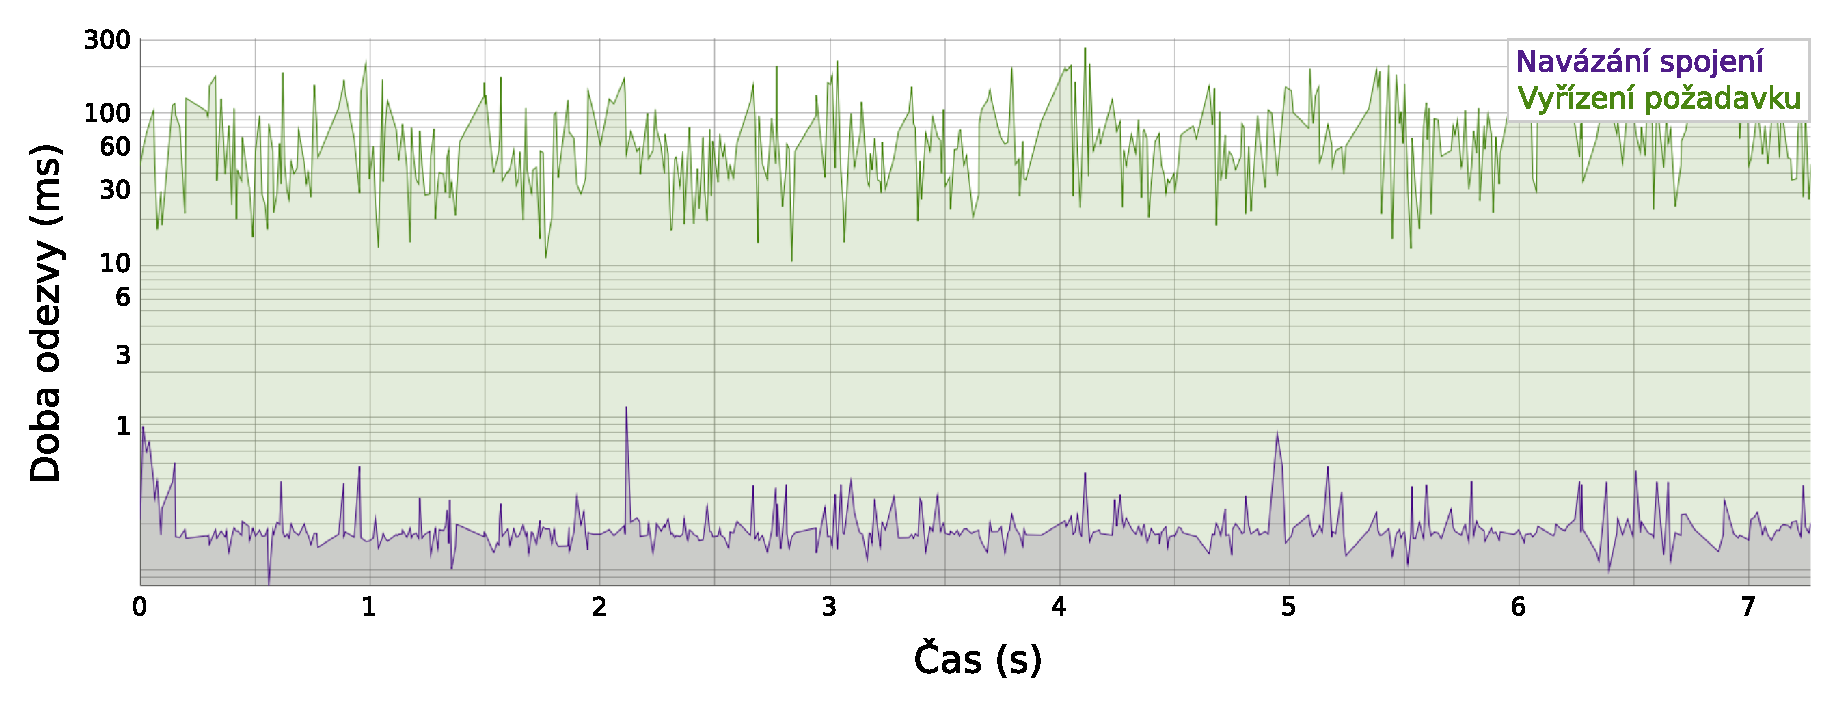
\includegraphics[width=\textwidth]{sniper.pdf}
\caption[Výsledky zátěžového testu]{Výsledky zátěžového testování -- doba odezvy v čase}
\label{sniper}
\end{figure}


%%%%%%%%%%%%%%%%%%%%%%%%%%%%
\chapter{Závěr}

Cílem této práce bylo vytvořit nástroj, který bude poskytovat textové vyhledávání jako službu a 
umožní provozovatelům elektronických obchodů snadnou implementaci vyhledávání, které si poradí
s problematikou přirozeného jazyka a zároveň bude dostatečně rychlé. Toho bylo dosaženo prostřednictvím
jednotlivých fází vývoje software -- analýzy problematiky, návrhu řešení, jeho implementace a nakonec
také otestování výsledné implementace.

Byl vytvořen nástroj, který je možné začít používat a dále jej rozvíjet, přičemž provozovatelům
elektronických obchodů jeho využití přináší významnou úsporu při vytváření takového nástroje
svépomocí. Toto zjednodušení je zřejmé také ve srovnání s konkurenčními službami, které většinou
nabízí univerzálnější nástroj, který nakonec ke kýženému zjednodušení nevede tak dobře.

\section{Dosažení vytyčených cílů}

V první části této práce byla \textbf{analyzována problematika elektronického obchodování}, vysvětleny pojmy
a vztahy mezi nimi -- jejich znalost je nutná pro vytvoření vyhledávání. Byl také analyzován stávající
způsob řešení textového vyhledávání, možnosti pro jeho zlepšení, srovnány stávající nástroje
umožňující řešení vyhledávání. V této práci vyvinutý nástroj řeší problém napojení ve směru
z elektronického obchodu využitím již existujících exportů. Díky tomu je toto napojení možné
bez zásahu IT oddělení, což je značnou úsporou v celém procesu. Obdobně je napojení opačným směrem navrženo 
tak, aby bylo implementovatelné s minimálním úsilím, bez nutnosti využívání dalších knihoven.

Dále byla \textbf{analyzována problematika textového vyhledávání}, vysvětlen princip indexace a rozebrány
jednotlivé problémy, které souvisí se zpracováním přirozeného jazyka. Aby přinášelo vyhledávání
skutečnou hodnotu, umí se vypořádat s tvaroslovím, překlepy nebo různými významy slov (synonymy).
Zároveň je možné zobrazovat výsledky vyhledávání již během psaní (funkce search-as-you-type), což
vede k lepšímu uživatelskému zážitku z vyhledávání.

Následně byl proveden \textbf{návrh aplikace}, který splňuje požadavky definované v analýze. Výstupem této
fáze jsou případy užití aplikace, datový model a dále také návrh struktury API. Právě rozdělení 
architektury na dvě části (backend disponující pouze API a frontend disponující grafickým rozhraním)
umožňuje zvolit pro každou část aplikace tu nejvhodnější technologii a dále aplikace vyvíjet, 
nasazovat a škálovat nezávisle na sobě, což vede k zrychlení vývojového cyklu.

Dále je aplikace na základě modelu \textbf{implementována}. Pro backend byl zvolen programovací jazyk
Go, který umožňuje dosáhnout krátkých časů odezvy API, zároveň je však dostatečně pohodlný
pro programátora, kdy se způsob jeho použití blíží práci s dynamickými jazyky. Díky rychlému
překladu je možné sestavený artifakt rychle nasazovat. Frontend je napsán v jazyce PHP, což
činí jeho zdrojový kód přehledným a snadno udržovatelným. Není problém však vyvinout novou verzi
v JavaScriptu a vytvořit tak tlustého klienta, který poběží pouze v okně webového prohlížeče.
Samotné vyhledávání probíhá v nástroji Elasticsearch, přičemž je popsán způsob jeho konfigurace
pro správnou funkci vyhovující požadavkům z analýzy. V této části práce je také popsán
způsob \textbf{nasazení aplikace} do produkčního prostředí, kdy je nakonfigurováno kontinuální
nasazování, které probíhá po každém nahrání kódu do vzdáleného repozitáře.

Nakonec je aplikace \textbf{otestována}, aby bylo ověřeno, zda vyhovuje zadání. Testy jsou děleny na tři
části -- nejprve je kontrolována snadnost implementace, popsány kroky, které je k napojení třeba 
provést a uveden je i časový odhad doby potřebné k napojení. Testována je samozřejmě i samotná
funkčnost vyhledávání, a to na konkrétních vyhledávacích dotazech nad reálnými daty. Nakonec
je ověřena samotná rychlost vyhledávání pomocí zátěžového testu, kdy průmerná doba odezvy aplikace
splňuje požadavky kladené na vyhledávání.

\section{Diskuze možného budoucího rozšiřování}

Aplikaci je samozřejmě možné dále rozšiřovat, přičemž směrů pro další zlepšování je více. První možností
je přidání obrazovky do administrátorského rozhraní, na které bude možné provést 
\textbf{úpravu parametrů vyhledávání daného uživatele}. To proto, že má každý obchod jinak nastavená pravidla 
na konkrétní funkčnost, například někdo nemusí chtít pracovat s našeptáváním nebo překlepy výměnou za zrychlení 
vyhledávání. Dále mohou obchody různě pracovat s významy slov (například s hantýrkou) a bylo by dobré jim
umožňit přidávat vlastní stop slova nebo synonyma. Takové informace by navíc mohly být užitečné
i pro ostatní obchody. Samotnou analýzou je totiž obtížné je získat -- provozovaných oborů obchodování
je nespočet.

Jednotlivé obchody však mohou mít i jiné požadavky na \textbf{řazení výsledků vyhledávání}, což už je 
komplexnější problématika. Pro někoho může být důležitější než jen relevance například to, že
má na daném produktu větší marži, nebo má smluvní vztah s dodavatelem zboží, kterému se zavazuje
k výraznější propagaci daných výrobků. Někdy to nemusí být ani řízeno výdělkem, ale povahou sortimentu
obchodu, kdy může být hlavní sortiment v nabídce upřednostnován před sortimentem doplňkovým. Do řazení
výsledků vyhledávání však mohou svým chováním promlouvat i samotní uživatelé, kdy analýzou jejich 
chování mohou být zjištěny vztahy mezi hledanými výrazy a produkty. Zde už přichází ke slovu
doporučovací systémy a strojové učení obecně.

Další možnou cestou ke zlepšení může být vytvoření administrace v programovacím jazyce, který běží kompletně
\textbf{ve webovém prohlížeči uživatele}. Výhodou takového řešení je zrychlení odezvy aplikace 
(není třeba při každé operaci komunikovat přes síť) a ušetření výkonu serverů, kdy jsou použity 
jen k distribuci statického obsahu. 

Za předpokladu výraznějšího používání aplikace by bylo vhodné se dále zaměřit na \textbf{infrastrukturu}, 
na které je provozována. Díky tomu, že jsou již artefakty distribuovány pomocí linuxových kontejnerů
je přechod do propracovanějšího prostředí snadný. Nabízí se využít pokročilejších orchestrátorů
kontejnerů nebo rovnou cloudového řešení. V takovém prostředí je možné definovat pravidla pro automatické
škálování a využít tak přesně tolik výpočetních zdrojů, kolik je v danou chvíli třeba. Pro
toto rozšiřování je výhodou použití Elasticsearch, kdy je možné automatizovat i škálování
tohoto úložiště. Díky jeho koncepci je přidávání dalších instancí snadné a není třeba složitě
upravovat existující konfiguraci.

%%%%%%%%%%%%%%%%%%%%%%%%%%%%
\appendix

\chapter{Terminologický slovník}

\begin{center}

\begin{tabular}{L{50mm} L{17mm} L{73mm}} 
\toprule
\textbf{Termín} & \textbf{Zkratka} & \textbf{Význam} \\
\midrule
Uniform Resource Locator & URL & Adresa dokumentu na webu\\
\hline
Extensible Markup Language & XML & Značkovací jazyk\\
\hline
European Article Number & EAN & Mezinárodní číselná identifikace výrobků\\
\hline
International Standard Book Number & ISBN & Číselná identifikace knižních vydání\\
\hline
Structured Query Language & SQL & Jazyk určený pro dotazování v relačních databázích\\
\hline
Hypertext Transfer Protocol & HTTP & Protokol pro přenos souborů po síti internet\\
\hline
Application Programming Interface & API & Rozhraní pro programování aplikací\\
\hline
Representational State Transfer & REST & Architektura rozhraní pro komunikaci mezi počítačovými systémy\\
\hline
Simple Object Access Protocol & SOAP & Protokol pro výměnu zpráv přes síť\\
\hline
Formální jazyk & & Množina konečných slov nad určitou abecedou\\
\hline
Počítačová lingvistika & & Obor na pomezí lingvistiky a informatiky -- věda o porozumění přirozenému jazyku\\
\hline
Morfologie & & Lingvistická disciplína zabývající se ohýbáním slov\\
\hline
Frontend & & Část aplikace s kterou uživatel přímo komunikuje prostřednictvím grafického rozhraní\\
\hline
Backend & & Část aplikace, která obstarává její logiku a persistenci dat\\
\bottomrule
\end{tabular}

\end{center}


\chapter{Obsah přiloženého CD}

\begin{center}

\begin{tabular}{L{67mm} L{73mm}} 
\toprule
\textbf{Soubor/složka} & \textbf{Popis} \\
\midrule
\verb|DP_Ludek_Vesely.pdf| & Text diplomové práce\\
\hline
\verb|DP_Ludek_Vesely-screencast.mov| & Ukázka použití aplikace koncovým uživatelem\\
\hline
\verb|src/backend| & Zdrojové kódy -- backend\\
\hline
\verb|src/frontend| & Zdrojové kódy -- frontend\\
\hline
\verb|src/elasticsearch| & Použitá distribuce Elasticsearch včetně konfiguračních souborů, slovníků a pluginů\\
\hline
\verb|src/docker-stack| & Konfigurace pro Docker Compose\\
\hline
\verb|src/tests| & Zdrojové kódy -- testovací skripty\\
\bottomrule
\end{tabular}

\vspace{15mm}

\textit{Veškeré zdrojové kódy jsou k~dispozici také online}\\
\textit{na URL: \url{https://github.com/apisearch}.}

\end{center}


%\chapter{Graf jako příloha}
%\begin{figure}[h]
%\center
%
\includegraphics[width=0.86\textwidth]{todo.pdf}
%\end{figure}


%%%%%%%%%%%%%%%%%%%%%%%%%%%%
\begin{thebibliography}{Mm99} \addcontentsline{toc}{chapter}{Literatura}

% e-commerce

\bibitem{e-commerce} SUCHÁNEK Petr. \emph{E-commerce}.
Vyd.~1. Praha: Ekopress, s.r.o., 2012 144~s. ISBN 978-80-86929-84-2.

% vyhledávání

\bibitem{strossa} STROSSA, Petr. \emph{Počítačové zpracování přirozeného jazyka}.
Vyd.~1. Praha: Oeconomica, 2011 316~s. ISBN 978-80-245-1777-3.

\bibitem{searching} AYSE Göker a DAVIES John.
\emph{Information Retrieval: Searching in the 21st Century}.
Vyd.~1. Library of Congress Cataloging-in-Publication Data, 2009 295~s. ISBN: 978-0-470-02762-2.

\bibitem{mining} AGGARWAL Charu C., ZHAI ChengXiang. \emph{Mining Text Data}.
Springer New York Dordrecht Heidelberg London, 2000 522~s. ISBN 978-1-4614-3222-7.

% elastic

\bibitem{es-guide} CLINTON Gormley, ZACHARY Tong. \emph{Elasticsearch: The Definitive Guide}.
O'Reilly Media, 2015 724~s. ISBN 978-1-4493-5854-9.

\bibitem{elastic-reference} ELASTIC. \emph{Elasticsearch Reference} [online].
2017 [cit. 2017-03-03]. Dostupné z:
\url{https://www.elastic.co/guide/en/elasticsearch/reference/current/index.html}

% api

\bibitem{api} STURGEON Phil. \emph{Build APIs You Won't Hate}.
Vyd.~1. Philip J. Sturgeon, 2015 188~s. ISBN 978-0692232699.

% go

\bibitem{go-in-action} KENNEDY William. \emph{Go in Action}.
Manning Publications Co, 2016 264~s. ISBN 978-1-6172-9178-4.

\bibitem{go-concurrency} KOZYRA Nathan. \emph{Mastering Concurrency in Go}.
Packt Publishing, 2014 301~s. ISBN-13 978-1783983483.

\bibitem{go-xml} ASTAXIE. \emph{Build web applications with Golang} [online].
2017 [cit. 2017-04-14]. Dostupné z: \url{https://astaxie.gitbooks.io/build-web-application-with-golang/en/07.1.html}.

% docker

\bibitem{docker} MATTHIAS Karl, KANE P. Sean. \emph{Docker: Up \& Running}.
O'Reilly Media, 2015 232~s. ISBN 978-1-4919-1754-1.

\bibitem{devops} FARCIC Viktor. \emph{The DevOps 2.0 Toolkit: Automating the Continuous Deployment Pipeline 
with Containerized Microservices}. Packt Publishing, 2016 462~s. ISBN 978-1-78528-031-3.

\bibitem{architecture} RICHARDS Mark. \emph{Software Architecture Patterns}.
O'Reilly Media, 2015 47~s. ISBN-13 978-1491924242.

% další...

\bibitem{apiary} APIARY. \emph{Platform for API Design, Development \& Documentation} [online].
2017 [cit. 2017-03-11]. Dostupné z: \url{https://apiary.io}.

\bibitem{elastic} ELASTIC. \emph{ Elasticsearch: RESTful, Distributed Search \& Analytics} [online].
2017 [cit. 2017-04-12]. Dostupné z: \url{https://www.elastic.co/products/elasticsearch}

\bibitem{algolia} ALGOLIA. \emph{Hosted cloud search as a service} [online].
2017 [cit. 2017-03-03]. Dostupné z:
\url{https://www.elastic.co/guide/en/elasticsearch/reference/current/index.html}

\bibitem{swiftype} SWIFTYPE. \emph{Site Search by Swiftype} [online].
2017 [cit. 2017-03-30]. Dostupné z: \url{https://swiftype.com/site-search}

\bibitem{cloud-search} AWS. \emph{Amazon CloudSearch} [online].
2017 [cit. 2017-03-30]. Dostupné z: \url{https://aws.amazon.com/cloudsearch}

\bibitem{gse} GOOGLE. \emph{Custom Search Engine} [online].
2017 [cit. 2017-03-30]. Dostupné z: \url{https://cse.google.com/cse}

\bibitem{amazon-100ms} GIGASPACES.
\emph{Amazon found every 100ms of latency cost them 1\% in sales} [online]. \\
2017 [cit. 2017-03-26].
Dostupné z: \url{https://blog.gigaspaces.com/amazon-found-every-100ms-of-latency-cost-them-1-in-sales}

\bibitem{stackshare-algolia} STACKSHARE, Inc. 
\emph{How Algolia Reduces Latency For 21B Searches Per Month} [online].\\
2017 [cit. 2017-04-05]. Dostupné z:
\url{https://stackshare.io/algolia/how-algolia-reduces-latency-for-21b-searches-per-month}

\bibitem{postgres} THE POSTGRESQL GLOBAL DEVELOPMENT GROUP. \emph{Documentation: Full Text Search} [online].\\
2017 [cit. 2017-03-26]. Dostupné z: \url{https://www.postgresql.org/docs/9.5/static/textsearch.html}

\bibitem{lucene} THE APACHE SOFTWARE FOUNDATION. \emph{Apache Lucene} [online].\\
2017 [cit. 2017-03-26]. Dostupné z: \url{https://lucene.apache.org}

\bibitem{netmonitor} SDRUŽENÍ PRO INTERNETOVÝ ROZVOJ. \emph{NetMonitor} [online].
2017 [cit. 2017-04-01]. Dostupné z: \url{http://www.netmonitor.cz}

\bibitem{xml-heureka} HEUREKA SHOPPING s.r.o. \emph{Specifikace XML souboru} [online].\\
2017 [cit. 2017-04-01]. Dostupné z: \url{https://sluzby.heureka.cz/napoveda/xml-feed}

\bibitem{xml-zbozi} SEZNAM.CZ, a.s. \emph{Specifikace XML feedu pro internetové obchody} [online].\\
2017 [cit. 2017-04-01]. Dostupné z:
\url{https://napoveda.seznam.cz/cz/zbozi/specifikace-xml-pro-obchody/specifikace-xml-feedu}

\bibitem{nejpouzivanejsi-slova} TĚŠITELOVÁ Marie. \emph{O češtině v číslech}.
Praha: Academia, 1987 205~s.

\bibitem{es-fuzziness} ELASTIC. \emph{The Definitive Guide - Fuzziness} [online].
2017 [cit. 2017-04-08]. Dostupné z:
\url{https://www.elastic.co/guide/en/elasticsearch/guide/current/fuzziness.html}.

\bibitem{damerau} DAMERAU, Fred J. \emph{A Technique for Computer Detection and Correction of Spelling Errors}.
Communications of the ACM (ACM), 1964, s. 171–176. ISSN 0001-0782. doi: 10.1145/363958.363994.
Dostupné z: \url{http://doi.acm.org/10.1145/363958.363994}

\bibitem{n-gram} SMETANIN Nikita. \emph{Fuzzy string search} [online].
2017 [cit. 2017-04-08]. 
Dostupné z: \url{http://ntz-develop.blogspot.cz/2011/03/fuzzy-string-search.html}.

\bibitem{christen} CHRISTEN, Peter. \emph{A Comparison of Personal Name Matching: Techniques and Practical Issues}.
ICDMW '06 Proceedings of the Sixth IEEE International Conference on Data Mining, 2006, s. 290-294,
IEEE Computer Society Washington, DC, USA. doi: 10.1145/363958.363994. 
Dostupné z: \url{http://users.cecs.anu.edu.au/~Peter.Christen/publications/tr-cs-06-02.pdf}. 
ISBN: 0-7695-2702-7.

\bibitem{backend} HUS Maarten. \emph{The case for separating front- and back-end} [online].
2014 [cit. 2017-04-11]. 
Dostupné z: \url{http://dontpanic.42.nl/2014/10/the-case-for-separating-front-and-back.html}.

\bibitem{apiary-design} APIARY. \emph{How to Build an API} [online].
2017 [cit. 2017-04-11]. Dostupné z: \url{https://apiary.io/how-to-build-api}.

\bibitem{scaling} IBM. \emph{How to explain vertical and horizontal scaling in the cloud} [online].
2014 [cit. 2017-04-11]. Dostupné z: 
\url{https://www.ibm.com/blogs/cloud-computing/2014/04/explain-vertical-horizontal-scaling-cloud}.

\bibitem{api-blueprint} API BLUEPRINT. \emph{A powerful high-level API description language for web APIs} [online].
2017 [cit. 2017-04-12]. Dostupné z: \url{https://apiblueprint.org}.

\bibitem{websockets} MOZILLA Developer Network. \emph{WebSockets -- Web APIs} [online].
2017 [cit. 2017-04-12]. Dostupné z: \url{https://developer.mozilla.org/en-US/docs/Web/API/WebSockets_API}.

\bibitem{postgres-search} THE POSTGRESQL GLOBAL DEVELOPMENT GROUP. 
\emph{Documentation: Chapter 12. Full Text Search} [online].
2017 [cit. 2017-04-12]. Dostupné z: \url{https://www.postgresql.org/docs/9.1/static/textsearch-intro.html}.

\bibitem{es-analysis} ELASTIC. \emph{Elasticsearch Reference: Analysis} [online].
2017 [cit. 2017-04-12]. Dostupné z: \url{https://www.elastic.co/guide/en/elasticsearch/reference/current/analysis.html}.

\bibitem{es-postgres} ROWE Nathaniel. 
\emph{Performance Testing a Postgres Database vs Elasticsearch 5: Column Statistics} [online].
2017 [cit. 2017-04-12]. Dostupné z: \url{http://blog.nrowegt.com/database-vs-elasticsearch-speed-column-statistics}.

\bibitem{es-postgres-2} ROWE Nathaniel. 
\emph{How To Use Sub Aggregations With Searchkick To Return Multiple Terms Per Document} [online].
2017 [cit. 2017-04-12]. Dostupné z: 
\url{http://blog.nrowegt.com/how-to-use-sub-aggregations-with-searchkick-to-return-multiple-terms-per-document}.

\bibitem{solr} THE APACHE SOFTWARE FOUNDATION. \emph{Apache Solr} [online].
2017 [cit. 2017-04-12]. Dostupné z: \url{http://lucene.apache.org/solr}.

\bibitem{es-solr} YIGAL Asaf. \emph{Solr vs. Elasticsearch: Who’s The Leading Open Source Search Engine?} [online].
2016 [cit. 2017-04-12]. Dostupné z: \url{https://logz.io/blog/solr-vs-elasticsearch}.

\bibitem{sphinx} SPHINX Technologies Inc. \emph{Sphinx Search} [online].
2017 [cit. 2017-04-12]. Dostupné z: \url{http://sphinxsearch.com}.

\bibitem{hunspell} NÉMETH László. \emph{Hunspell} [online].
2017 [cit. 2017-04-13]. Dostupné z: \url{http://hunspell.github.io}.

\bibitem{hunspell-man} CANONICAL Ltd. 
\emph{Ubuntu Manpage: hunspell - format of Hunspell dictionaries and affix files} [online].
2017 [cit. 2017-04-13]. Dostupné z: \url{http://manpages.ubuntu.com/manpages/trusty/en/man4/hunspell.4.html}.

\bibitem{alpine} ALPINE Linux Development Team. \emph{Alpine Linux} [online].
2017 [cit. 2017-04-13]. Dostupné z: \url{https://alpinelinux.org}.

\bibitem{alpine-lean} WALLIN Marko. \emph{Lean Docker Containers with Alpine Linux} [online].
2017 [cit. 2017-04-13]. Dostupné z: \url{https://gofore.com/en/lean-docker-alpine-linux}.

\bibitem{circleci} CIRCLE CI. \emph{Continuous Integration and Delivery} [online].
2017 [cit. 2017-04-14]. Dostupné z: \url{https://circleci.com}.

\bibitem{compose} DOCKER. \emph{Compose: Define and run multi-container applications with Docker} [online].
2017 [cit. 2017-04-14]. Dostupné z: \url{https://github.com/docker/compose}.

\bibitem{hunspell-download} THE APACHE SOFTWARE FOUNDATION. \emph{Apache OpenOffice: Index of /contrib/dictionaries}
[online]. 2017 [cit. 2017-04-17]. Dostupné z: \url{http://download.services.openoffice.org/contrib/dictionaries}.

\bibitem{wordnet} EUROPEAN LANGUAGE RESOURCES ASSOCIATION. \emph{Czech WordNet} [online].
2017 [cit. 2017-04-17]. Dostupné z: \url{http://catalog.elra.info/product_info.php?products_id=1089}.

\bibitem{es-suggester} ELASTIC. \emph{Completion Suggester} [online].
2017 [cit. 2017-04-17]. Dostupné z: 
\url{https://www.elastic.co/guide/en/elasticsearch/reference/current/search-suggesters-completion.html}.

\bibitem{sniper} BTFAK. \emph{A powerful \& high-performance http load tester} [online].
2017 [cit. 2017-04-19]. Dostupné z: \url{https://github.com/btfak/sniper}.

\bibitem{ab} THE APACHE SOFTWARE FOUNDATION. \emph{ab - Apache HTTP server benchmarking tool} [online].
2017 [cit. 2017-04-19]. Dostupné z: \url{http://httpd.apache.org/docs/current/programs/ab.html}.

\end{thebibliography}


%%%%%%%%%%%%%%%%%%%%%%%%%%%%
\end{document}
